\documentclass[a4paper]{article}

\def\npart {III}
\def\nterm {Michaelmas}
\def\nyear {2017}
\def\nlecturer {R.\ D.\ Shah}
\def\ncourse {Modern Statistical Methods}
\def\nofficial {https://www.dpmms.cam.ac.uk/~rds37/modern_stat_methods.html}

% Imports
\ifx \nextra \undefined
  \usepackage[pdftex,
    hidelinks,
    pdfauthor={Dexter Chua},
    pdfsubject={Cambridge Maths Notes: Part \npart\ - \ncourse},
    pdftitle={Part \npart\ - \ncourse},
  pdfkeywords={Cambridge Mathematics Maths Math \npart\ \nterm\ \nyear\ \ncourse}]{hyperref}
  \title{Part \npart\ - \ncourse}
\else
  \usepackage[pdftex,
    hidelinks,
    pdfauthor={Dexter Chua},
    pdfsubject={Cambridge Maths Notes: Part \npart\ - \ncourse\ (\nextra)},
    pdftitle={Part \npart\ - \ncourse\ (\nextra)},
  pdfkeywords={Cambridge Mathematics Maths Math \npart\ \nterm\ \nyear\ \ncourse\ \nextra}]{hyperref}

  \title{Part \npart\ - \ncourse \\ {\Large \nextra}}
\fi

\author{Lectured by \nlecturer \\\small Notes taken by Dexter Chua}
\date{\nterm\ \nyear}

\usepackage{alltt}
\usepackage{amsfonts}
\usepackage{amsmath}
\usepackage{amssymb}
\usepackage{amsthm}
\usepackage{booktabs}
\usepackage{caption}
\usepackage{enumitem}
\usepackage{fancyhdr}
\usepackage{graphicx}
\usepackage{mathtools}
\usepackage{microtype}
\usepackage{multirow}
\usepackage{pdflscape}
\usepackage{pgfplots}
\usepackage{siunitx}
\usepackage{tabularx}
\usepackage{tikz}
\usepackage{tkz-euclide}
\usepackage[normalem]{ulem}
\usepackage[all]{xy}

\pgfplotsset{compat=1.12}

\pagestyle{fancyplain}
\lhead{\emph{\nouppercase{\leftmark}}}
\ifx \nextra \undefined
  \rhead{
    \ifnum\thepage=1
    \else
      \npart\ \ncourse
    \fi}
\else
  \rhead{
    \ifnum\thepage=1
    \else
      \npart\ \ncourse\ (\nextra)
    \fi}
\fi
\usetikzlibrary{arrows}
\usetikzlibrary{decorations.markings}
\usetikzlibrary{decorations.pathmorphing}
\usetikzlibrary{positioning}
\usetikzlibrary{fadings}
\usetikzlibrary{intersections}
\usetikzlibrary{cd}

\newcommand*{\Cdot}{\raisebox{-0.25ex}{\scalebox{1.5}{$\cdot$}}}
\newcommand {\pd}[2][ ]{
  \ifx #1 { }
    \frac{\partial}{\partial #2}
  \else
    \frac{\partial^{#1}}{\partial #2^{#1}}
  \fi
}

% Theorems
\theoremstyle{definition}
\newtheorem*{aim}{Aim}
\newtheorem*{axiom}{Axiom}
\newtheorem*{claim}{Claim}
\newtheorem*{cor}{Corollary}
\newtheorem*{defi}{Definition}
\newtheorem*{eg}{Example}
\newtheorem*{fact}{Fact}
\newtheorem*{law}{Law}
\newtheorem*{lemma}{Lemma}
\newtheorem*{notation}{Notation}
\newtheorem*{prop}{Proposition}
\newtheorem*{thm}{Theorem}

\renewcommand{\labelitemi}{--}
\renewcommand{\labelitemii}{$\circ$}
\renewcommand{\labelenumi}{(\roman{*})}

\let\stdsection\section
\renewcommand\section{\newpage\stdsection}

% Strike through
\def\st{\bgroup \ULdepth=-.55ex \ULset}

% Maths symbols
\newcommand{\bra}{\langle}
\newcommand{\ket}{\rangle}

\newcommand{\N}{\mathbb{N}}
\newcommand{\Z}{\mathbb{Z}}
\newcommand{\Q}{\mathbb{Q}}
\renewcommand{\H}{\mathbb{H}}
\newcommand{\R}{\mathbb{R}}
\newcommand{\C}{\mathbb{C}}
\newcommand{\Prob}{\mathbb{P}}
\renewcommand{\P}{\mathbb{P}}
\newcommand{\E}{\mathbb{E}}
\newcommand{\F}{\mathbb{F}}
\newcommand{\cU}{\mathcal{U}}
\newcommand{\RP}{\mathbb{RP}}
\newcommand{\CP}{\mathbb{CP}}

\newcommand{\ph}{\,\cdot\,}

\DeclareMathOperator{\sech}{sech}
\DeclareMathOperator{\cosech}{cosech}
\DeclareMathOperator{\cosec}{cosec}

\DeclareMathOperator{\covol}{covol}
\DeclareMathOperator{\vol}{vol}

\let\Im\relax
\let\Re\relax
\DeclareMathOperator{\Im}{Im}
\DeclareMathOperator{\Re}{Re}
\DeclareMathOperator{\im}{im}
\DeclareMathOperator{\image}{image}
\DeclareMathOperator{\Ann}{Ann}

\DeclareMathOperator*{\res}{res}
\DeclareMathOperator{\Res}{Res}
\DeclareMathOperator{\Ind}{Ind}

\DeclareMathOperator{\tr}{tr}
\DeclareMathOperator{\diag}{diag}
\DeclareMathOperator{\rank}{rank}
\DeclareMathOperator{\card}{card}
\DeclareMathOperator{\spn}{span}
\DeclareMathOperator{\adj}{adj}

\DeclareMathOperator{\erf}{erf}
\DeclareMathOperator{\erfc}{erfc}

\DeclareMathOperator{\ord}{ord}
\DeclareMathOperator{\Sym}{Sym}

\DeclareMathOperator{\sgn}{sgn}
\DeclareMathOperator{\orb}{orb}
\DeclareMathOperator{\stab}{stab}
\DeclareMathOperator{\ccl}{ccl}

\DeclareMathOperator{\lcm}{lcm}
\DeclareMathOperator{\hcf}{hcf}

\DeclareMathOperator{\Int}{Int}
\DeclareMathOperator{\id}{id}

\DeclareMathOperator{\betaD}{beta}
\DeclareMathOperator{\gammaD}{gamma}
\DeclareMathOperator{\Poisson}{Poisson}
\DeclareMathOperator{\binomial}{binomial}
\DeclareMathOperator{\multinomial}{multinomial}
\DeclareMathOperator{\Bernoulli}{Bernoulli}
\DeclareMathOperator{\like}{like}

\DeclareMathOperator{\var}{var}
\DeclareMathOperator{\cov}{cov}
\DeclareMathOperator{\bias}{bias}
\DeclareMathOperator{\mse}{mse}
\DeclareMathOperator{\corr}{corr}

\DeclareMathOperator{\otp}{otp}
\DeclareMathOperator{\dom}{dom}

\DeclareMathOperator{\Root}{Root}
\DeclareMathOperator{\supp}{supp}
\DeclareMathOperator{\rel}{rel}
\DeclareMathOperator{\Hom}{Hom}
\DeclareMathOperator{\Aut}{Aut}
\DeclareMathOperator{\Gal}{Gal}
\DeclareMathOperator{\Mat}{Mat}
\DeclareMathOperator{\End}{End}
\DeclareMathOperator{\Char}{char}
\DeclareMathOperator{\ev}{ev}
\DeclareMathOperator{\St}{St}
\DeclareMathOperator{\Lk}{Lk}
\DeclareMathOperator{\disc}{disc}
\DeclareMathOperator{\Isom}{Isom}
\DeclareMathOperator{\length}{length}
\DeclareMathOperator{\energy}{energy}
\DeclareMathOperator{\area}{area}
\DeclareMathOperator{\Syl}{Syl}
\DeclareMathOperator{\cl}{cl}
\DeclareMathOperator{\fix}{fix}

\newcommand{\GL}{\mathrm{GL}}
\newcommand{\SL}{\mathrm{SL}}
\newcommand{\PGL}{\mathrm{PGL}}
\newcommand{\PSL}{\mathrm{PSL}}
\newcommand{\PSU}{\mathrm{PSU}}
\newcommand{\Or}{\mathrm{O}}
\newcommand{\SO}{\mathrm{SO}}
\newcommand{\U}{\mathrm{U}}
\newcommand{\SU}{\mathrm{SU}}

\renewcommand{\d}{\mathrm{d}}
\newcommand{\D}{\mathrm{D}}

\tikzset{->/.style = {decoration={markings,
                                  mark=at position 1 with {\arrow[scale=2]{latex'}}},
                      postaction={decorate}}}
\tikzset{<-/.style = {decoration={markings,
                                  mark=at position 0 with {\arrowreversed[scale=2]{latex'}}},
                      postaction={decorate}}}
\tikzset{<->/.style = {decoration={markings,
                                   mark=at position 0 with {\arrowreversed[scale=2]{latex'}},
                                   mark=at position 1 with {\arrow[scale=2]{latex'}}},
                       postaction={decorate}}}
\tikzset{->-/.style = {decoration={markings,
                                   mark=at position #1 with {\arrow[scale=2]{latex'}}},
                       postaction={decorate}}}
\tikzset{-<-/.style = {decoration={markings,
                                   mark=at position #1 with {\arrowreversed[scale=2]{latex'}}},
                       postaction={decorate}}}

\tikzset{circ/.style = {fill, circle, inner sep = 0, minimum size = 3}}
\tikzset{mstate/.style={circle, draw, blue, text=black, minimum width=0.7cm}}

\definecolor{mblue}{rgb}{0.2, 0.3, 0.8}
\definecolor{morange}{rgb}{1, 0.5, 0}
\definecolor{mgreen}{rgb}{0.1, 0.4, 0.2}
\definecolor{mred}{rgb}{0.5, 0, 0}

\def\drawcirculararc(#1,#2)(#3,#4)(#5,#6){%
    \pgfmathsetmacro\cA{(#1*#1+#2*#2-#3*#3-#4*#4)/2}%
    \pgfmathsetmacro\cB{(#1*#1+#2*#2-#5*#5-#6*#6)/2}%
    \pgfmathsetmacro\cy{(\cB*(#1-#3)-\cA*(#1-#5))/%
                        ((#2-#6)*(#1-#3)-(#2-#4)*(#1-#5))}%
    \pgfmathsetmacro\cx{(\cA-\cy*(#2-#4))/(#1-#3)}%
    \pgfmathsetmacro\cr{sqrt((#1-\cx)*(#1-\cx)+(#2-\cy)*(#2-\cy))}%
    \pgfmathsetmacro\cA{atan2(#2-\cy,#1-\cx)}%
    \pgfmathsetmacro\cB{atan2(#6-\cy,#5-\cx)}%
    \pgfmathparse{\cB<\cA}%
    \ifnum\pgfmathresult=1
        \pgfmathsetmacro\cB{\cB+360}%
    \fi
    \draw (#1,#2) arc (\cA:\cB:\cr);%
}
\newcommand\getCoord[3]{\newdimen{#1}\newdimen{#2}\pgfextractx{#1}{\pgfpointanchor{#3}{center}}\pgfextracty{#2}{\pgfpointanchor{#3}{center}}}

\def\Xint#1{\mathchoice
   {\XXint\displaystyle\textstyle{#1}}%
   {\XXint\textstyle\scriptstyle{#1}}%
   {\XXint\scriptstyle\scriptscriptstyle{#1}}%
   {\XXint\scriptscriptstyle\scriptscriptstyle{#1}}%
   \!\int}
\def\XXint#1#2#3{{\setbox0=\hbox{$#1{#2#3}{\int}$}
     \vcenter{\hbox{$#2#3$}}\kern-.5\wd0}}
\def\ddashint{\Xint=}
\def\dashint{\Xint-}


\DeclareMathOperator*\argmin{argmin}
\DeclareMathOperator\pa{pa}
\DeclareMathOperator\child{ch}
\DeclareMathOperator\de{de}
\newcommand\ddo{\mathsf{do}}
\tikzset{msstate/.style={circle, draw, blue, text=black, minimum width=0.5cm}}

\begin{document}
\maketitle
{\small
\setlength{\parindent}{0em}
\setlength{\parskip}{1em}

The remarkable development of computing power and other technology now allows scientists and businesses to routinely collect datasets of immense size and complexity. Most classical statistical methods were designed for situations with many observations and a few, carefully chosen variables. However, we now often gather data where we have huge numbers of variables, in an attempt to capture as much information as we can about anything which might conceivably have an influence on the phenomenon of interest. This dramatic increase in the number variables makes modern datasets strikingly different, as well-established traditional methods perform either very poorly, or often do not work at all.

Developing methods that are able to extract meaningful information from these large and challenging datasets has recently been an area of intense research in statistics, machine learning and computer science. In this course, we will study some of the methods that have been developed to analyse such datasets. We aim to cover some of the following topics.

\begin{itemize}
  \item Kernel machines: the kernel trick, the representer theorem, support vector machines, the hashing trick.
  \item Penalised regression: Ridge regression, the Lasso and variants.
  \item Graphical modelling: neighbourhood selection and the graphical Lasso. Causal inference through structural equation modelling; the PC algorithm.
  \item High-dimensional inference: the closed testing procedure and the Benjamini--Hochberg procedure; the debiased Lasso
\end{itemize}

\subsubsection*{Pre-requisites}
Basic knowledge of statistics, probability, linear algebra and real analysis. Some background in optimisation would be helpful but is not essential.
}
\tableofcontents

\setcounter{section}{-1}
\section{Introduction}
In recent years, there has been a rather significant change in what sorts of data we have to handle and what questions we ask about them, witnessed by the popularity of the buzzwords ``big data'' and ``machine learning''. In classical statistics, we usually have a small set of parameters, and a very large data set. We then use the large data set to estimate the parameters.

However, nowadays we often see scenarios where we have a very large number of parameters, and the data set is relatively small. If we tried to apply our classical linear regression, then we would just be able to tune the parameters so that we have a perfect fit, and still have great freedom to change the parameters without affecting the fitting.

One example is that we might want to test which genomes are responsible for a particular disease. In this case, there is a huge number of genomes to consider, and there is good reason to believe that most of them are irrelevant, i.e.\ the parameters should be set to zero. Thus, we want to develop methods that find the ``best'' fitting model that takes this into account.

Another problem we might encounter is that we just have a large data set, and doing linear regression seems a bit silly. If we have so much data, we might as well try to fit more complicated curves, such as polynomial functions and friends. Perhaps more ambitiously, we might try to find the best \emph{continuously differentiable function} that fits the curve, or, as analysts will immediately suggest as an alternative, weakly differentiable functions.

There are many things we can talk about, and we can't talk about all of them. In this course, we are going to cover $4$ different topics of different size:
\begin{itemize}
  \item Kernel machines
  \item The Lasso and its extensions
  \item Graphical modeling and causal inference
  \item Multiple testing and high-dimensional inference
\end{itemize}
The four topics are rather disjoint, and draw on different mathematical skills.

\section{Classical statistics}
This is a course on \emph{modern} statistical methods. Before we study methods, we give a brief summary of what we are \emph{not} going to talk about, namely classical statistics.

So suppose we are doing regression. We have some \term{predictors} $x_i \in \R^p$ and \term{responses} $Y_i \in \R$, and we hope to find a model that describes $Y$ as a function of $x$. For convenience, define the vectors
\[
  X = \begin{pmatrix} x_1^T \\ \vdots \\ x_n^T\end{pmatrix},\quad
  Y = \begin{pmatrix} Y_1^T \\ \vdots \\ Y_n^T\end{pmatrix}.
\]
The linear model then assumes there is some $\beta^0 \in \R^p$ such that
\[
  Y = X \beta^0 + \varepsilon,
\]
where $\varepsilon$ is some (hopefully small) error random variable. Our goal is then to estimate $\beta^0$ given the data we have.

If $X$ has full column rank, so that $X^TX$ is invertible, then we can use \term{ordinary least squares} to estimate $\beta^0$, with estimate
\[
  \hat{\beta}^{OLS} = \argmin_{\beta \in \R^p} \|Y - x \beta\|_2^2 = (X^TX)^{-1} X^TY.
\]
This assumes nothing about $\varepsilon$ itself, but if we assume that $\E \varepsilon = 0$ and $\var (\mathcal{E}) = \sigma^2 I$, then this estimate satisfies
\begin{itemize}
  \item $\E_\beta \hat{\beta}^{OLS} = (X^T X)^{-1} X^T X \beta^0 = \beta^0$
  \item $\var_\beta(\hat{\beta}^{OLS}) = (X^T X^{-1}) X^T \var(\varepsilon) X (X^T X)^{-1} = \sigma^2 (X^T X)^{-1}$.
\end{itemize}
In particular, this is an unbiased estimator. Even better, this is the best linear unbiased estimator. More precisely, the Gauss--Markov theorem says any other linear estimator $\tilde{\beta} = AY$ has $\var(\tilde{\beta}) - \var(\hat{\beta}^{OLS})$ positive semi-definite.

Of course, ordinary least squares is not the only way to estimate $\beta^0$. Another common method for estimating parameters is maximum likelihood estimation, and this works for more general models than linear regression. For people who are already sick of meeting likelihoods, this will be the last time we meet likelihoods in this course.

Suppose we want to estimate a parameter $\theta$ via knowledge of some data $Y$. We assume $Y$ has density $f(y; \theta)$. We define the \term{log-likelihood} by
\[
  \ell(\theta) = \log f(Y, \theta).
\]
The \term{maximum likelihood estimator} then maximize $\ell(\theta)$ over $\theta$ to get $\hat{\theta}$.

Similar to ordinary least squares, there is a theorem that says maximum likelihood estimation is the ``best''. To do so, we introduce the \term{Fisher information matrix}. This is a family of $d \times d$ matrices indexed by $\theta$, defined by
\[
  I_{jk}(\theta) = - E_\theta\left[\frac{\partial^2}{\partial \theta_j \partial \theta_j} \ell(\theta)\right].
\]
The relevant theorem is
\begin{thm}[Cram\'er--Rao bound]\index{Cram\'er--Rao bound}
  If $\tilde{\theta}$ is an unbiased estimator for $\theta$, then $\var(\tilde{\theta}) - I^{-1}(\theta)$ is positive semi-definite.

  Moreover, asymptotically, as $n \to \infty$, the maximum likelihood estimator is unbiased and achieves the Carm\'er--Rao bound.
\end{thm}

Another wonderful fact about the maximum likelihood estimator is that asymptotically, it is normal distributed, and so it is something we understand well.

This might seem very wonderful, but there are a few problems here. The results we stated are asymptotic, but what we actually see in real life is that as $n \to \infty$, the value of $p$ also increases. In these contexts, the asymptotic property doesn't tell us much. Another issue is that these all talk about unbiased estimators. In a lot of situations of interest, it turns out biased methods do much much better than these methods we have.

Another thing we might be interested is that as $n$ gets large, we might want to use more complicated models than simple parametric models, as we have much more data to mess with. This is not something ordinary least squares provides us with.

\section{Kernel machines}
We are going to start a little bit slowly, and think about our linear model $Y = X\beta^0 + \varepsilon$, where $\E(\varepsilon) = 0$ and $\var(\varepsilon) = \sigma^2 I$. Ordinary least squares is an unbiased estimator, so let's look at biased estimators.

For a biased estimator, $\tilde{\beta}$, we should not study the variance, but the \term{mean squared error}
\begin{align*}
  \E[(\tilde{\beta} - \beta^0)(\tilde{\beta} - \beta^0)^T]
  &= \E(\tilde{\beta} - \E \tilde{\beta} + E \tilde{\beta} - \beta^0)(\tilde{\beta} - \E \tilde{\beta} + E \tilde{\beta} - \beta^0)^T \\ &= \var(\tilde{\beta})+ (\E \tilde{\beta} - \beta^0)(\E \tilde{\beta} - \beta^0)^T
\end{align*}
The first term is, of course, just the variance, and the second is the squared bias. So the point is that if we pick a clever biased estimator with a tiny variance, then this might do better than unbiased estimators with large variance.

\subsection{Ridge regression}
Ridge regression was introduced in around 1970. The idea of Ridge regression is to try to shrink our estimator a bit in order to lessen the variance, at the cost of introducing a bias. We would hope then that this will result in a smaller mean squared error.

\begin{defi}[Ridge regression]
  \term{Ridge regression} solves
  \[
    (\hat{\mu}^R_\lambda, \hat{\beta}^R_\lambda) = \argmin_{(\mu, \beta) \in \R \times \R^p} \{ \|Y - \mu \mathbf{1} - X \beta\|_2^2 + \lambda \|\beta\|_2^2\},
  \]
  where $\mathbf{1}$ is a vector of all $1$'s. Here $\lambda \geq 0$ is a tuning parameter, and it controls how much we penalize a large choice of $\beta$.
\end{defi}

Here we explicitly have an intercept term. Usually, we eliminate this by adding a column of $1$'s in $X$. But here we want to separate that out, since we do not want give a penalty for large $\mu$. For example, if the parameter is temperature, and we decide to measure in degrees Celsius rather than Kelvins, then we don't want the resulting $\hat{\mu}, \hat{\beta}$ to change.

More precisely, our formulation of Ridge regression is so that if we make the modification
\[
  Y' = c\mathbf{1} + Y,
\]
then we have
\[
  \hat{\mu}^R_\lambda(Y') = \hat{\mu}_\lambda^R(Y) + c.
\]
Note also that the Ridge regression formula makes sense only if each entry in $\beta$ have the same order of magnitude, or else the penalty will only have a significant effect on the terms of large magnitude. Standard practice is to subtract from each column of $X$ its mean, and then scale it to have $\ell_2$ norm $\sqrt{n}$. The actual number is not important here, but it will in the case of the Lasso.

By differentiating, one sees that the solution to the optimization problem is
\begin{align*}
  \hat{\mu}_\lambda^R &= \bar{Y} = \frac{1}{n} \sum Y_i\\
  \hat{\beta}^R_\lambda &= (X^T X + \lambda I)^{-1} X^T Y.
\end{align*}
Note that we can always pick $\lambda$ such that the matrix $(X^T X + \lambda I)$ is invertible. In particular, this can work even if we have more parameters than data points. This will be important when we work with the Lasso later on.

If some god-like being told us a suitable value of $\lambda$ to use, then Ridge regression always works better than ordinary least squares.
\begin{thm}
  Suppose $\rank(X) = p$. Then for $\lambda > 0$ sufficiently small (depending on $\beta^0$ and $\sigma^2$), the matrix
  \[
    \E(\hat{\beta}^{OLS} - \beta^0)(\hat{\beta}^{OLS} - \beta^0)^T - \E(\hat{\beta}^{R}_\lambda - \beta^0)(\hat{\beta}^{R}_\lambda - \beta^0)^T \tag{$*$}
  \]
  is positive definite.
\end{thm}

\begin{proof}
  We know that the first term is just $\sigma^2(X^T X)^{-1}$. The right-hand-side has a variance term and a bias term. We first look at the bias:
  \begin{align*}
    \E [\hat{\beta} - \beta^0] &= (X^T X + \lambda I)^{-1} X^T X \beta^0 - \beta^0\\
    &= (X^T X + \lambda I)^{-1}(X^T X + \lambda I - \lambda I) \beta^0- \beta^0\\
    &= - \lambda (X^T X + \lambda I)^{-1} \beta^0.
  \end{align*}
  We can also compute the variance
  \[
    \var(\hat{\beta}) = \sigma^2(X^T X + \lambda I)^{-1} X^T X (X^T X + \lambda I)^{-1}.
  \]
  Note that both terms appearing in the squared error look like
  \[
    (X^T X + \lambda I)^{-1}\text{something}(X^T X + \lambda I)^{-1}.
  \]
  So let's try to write $\sigma^2 (X^T X)^{-1}$ in this form. Note that
  \begin{align*}
    (X^T X)^{-1} &= (X^T X + \lambda I)^{-1} (X^T X + \lambda I) (X^T X)^{-1} (X^T X + \lambda I) (X^T X + \lambda I)^{-1}\\
    &= (X^T X + \lambda I)^{-1}(X^T X + 2 \lambda I + \lambda^2 (X^T X)^{-1}) (X^T X + \lambda I)^{-1}.
  \end{align*}
  Thus, we can write $(*)$ as
  \begin{align*}
    &\hphantom{ {} = {} }(X^T X + \lambda I)^{-1} \Big( \sigma^2(X^T X + 2 \lambda I + \lambda^2(X^T X)^{-1})\\
    &\hphantom{adasdfafdasfdfadsfasdf}- \sigma^2 X^T X - \lambda^2 \beta^0 (\beta^0)^T\Big) (X^T X + \lambda I)^{-1}\\
    &= \lambda (X^T X + \lambda I)^{-1} \Big( 2 \sigma^2 I + \lambda(X^T X)^{-1} - \lambda \beta^0 (\beta^0)^T\Big) (X^T X + \lambda I)^{-1}
  \end{align*}
  Since $\lambda > 0$, this is positive definite iff
  \[
    2 \sigma^2 I + \sigma^2 \lambda (X^T X)^{-1} - \lambda \beta^0 (\beta^0)^T
  \]
  is positive definite, which is true for $0 < \lambda < \frac{2\sigma^2}{\|\beta^0\|_2^2}$.
\end{proof}
While this is nice, this is not really telling us much, because we don't know how to pick the correct $\lambda$. It also doesn't tell us when we should expect a big improvement from Ridge regression.

To understand this better, we need to use the \emph{singular value decomposition}.

\begin{thm}[Singular value decomposition]\index{singular value decomposition}\index{SVD}
  Let $X \in \R^{n \times p}$ be any matrix. Then it has a \emph{singular value decomposition} (SVD)
  \[
    \underset{n \times p}{X} = \underset{n \times n}{U}\;\;\underset{n \times p}{D}\;\;\underset{p \times p}{V^T},
  \]
  where $U, V$ are orthogonal matrices, and $D_{11} \geq D_{22} \geq \cdots \geq D_{mm} \geq 0$, where $m = \min (n, p)$, and all other entries of $D$ are zero.
\end{thm}

When $n > p$, there is an alternative version where $U$ is an $n \times p$ matrix with orthogonal columns, and $D$ is a $p \times p$ diagonal matrix. This is done by replacing $U$ by its first $p$ columns and $D$ by its first $p$ rows. This is known as the \term{thin singular value decomposition}\index{thin SVD}. In this case, $U^T U = I_p$ but $UU^T$ is not the identity.

Let's now apply try to understand Ridge regressions a little better. Suppose $n > p$. Then using the thin SVD, the fitted values from ridge regression are
\begin{align*}
  X \hat{\beta}_\lambda^R &= X (X^T X + \lambda I)^{-1} X^T Y\\
  &= UDV^T (VD^2 V^T + \lambda I)^{-1} VDU^T Y.
\end{align*}
We now note that $VD^2 V^T + \lambda I = V(D^2 + \lambda I)V^T$, since $V$ is still orthogonal. We then have
\[
  (V (D^2 + \lambda I)V^T)^{-1} = V(D^2 + \lambda I)^{-1} V^T
\]
Since $D^2$ and $\lambda I$ are both diagonal, it is easy to compute their inverses as well. We then have
\[
  X\hat{\beta}_\lambda^R = UD^2 (D^2 + \lambda I)^{-1} U^T Y = \sum_{j = 1}^p U_j \frac{D_{jj}^2}{ D_{jj}^2 + \lambda} U_j^T Y
\]
Here $U_j$ refers to the $j$th column of $U$.

Now note that the columns of $U$ form an orthonormal basis for the column space of $X$. If $\lambda = 0$, then this is just a fancy formula for the projection of $Y$ onto the column space of $X$. Thus, what this formula is telling us is that we look at this projection, look at the coordinates in terms of the basis given by the columns of $U$, and scale accordingly.

We can now concretely see the effect of our $\lambda$. The shrinking depends on the size of $D_{jj}$, and the larger $D_{jj}$ is, the less shrinking we do.

This is not very helpful if we don't have a concrete interpretation of the $D_{jj}$, or rather, the columns of $U$. It turns out the columns of $U$ are what are known as the \term{normalized principal components} of $X$.

Take $u \in \R^p$, $\|u\|_2 = 1$. The sample variance of $Xu \in \R^n$ is then
\[
  \frac{1}{n} \|Xu\|_2^2 = \frac{1}{n} u^T X^T X u = \frac{1}{n} u^T VD^2 V^t u.
\]
We write $w = V^T u$. Then $\|w\|_2 = 1$ since $V$ is orthogonal. So we have
\[
  \frac{1}{n} \|Xu\|_2^2 = \frac{1}{n} w^T D^2 w = \frac{1}{n} \sum_j w_j^2 D_{jj^2} \leq \frac{1}{n} D_{11}^2,
\]
and the bound is achieved when $w = e_1$, or equivalently, $u = V e_1 = V_1$. Thus, $V_1$ gives the coefficients of the linear combination of columns of $X$ that has largest sample variance. We can then write the result as
\[
  X V_1 = U DV^T V_1 = U_1 D_{11}.
\]
We can extend this to a description of the other columns of $U$, which is done in the example sheet. Roughly, the subsequent principle components obey the same optimality conditions with the added constraint of being orthogonal to all earlier principle components.

The conclusion is that Ridge regression works best if $\E Y$ lies in the space spanned by the large principal components of $X$. % insert example?

\subsection{\texorpdfstring{$v$}{v}-fold cross-validation}
In practice, the above analysis is not very useful, since it doesn't actually tell us what $\lambda$ we should pick. If we are given a concrete data set, how do we know what $\lambda$ we should pick?

One common method is to use \term{$v$-fold cross-validation}. This is a very general technique that allows us to pick a regression method from a variety of options. We shall explain the method in terms of Ridge regression, where our regression methods are parametrized by a single parameter $\lambda$, but it should be clear that this is massively more general.

Suppose we have some data set $(Y_i, x_i)_{i = 1}^n$, and we are asked to predict the value of $Y^*$ given a new predictors $x^*$. We may want to pick $\lambda$ to minimize the following quantity:
\[
  \E \left\{ (Y^* - (x^*)^T \hat{\beta}_\lambda^R(X, Y))^2 \mid X, Y \right\}.
\]
It is difficult to actually do this, and so an easier target to minimize is the expected prediction error
\[
  \E\left[\E \left\{ (Y^* - (x^*)^T \hat{\beta}_\lambda^R(\tilde{X}, \tilde{Y}))^2 \mid \tilde{X}, \tilde{Y} \right\}\right]
\]
One thing to note about this is that we are thinking of $\tilde{X}$ and $\tilde{Y}$ as arbitrary data sets of size $n$, as opposed to the one we have actually got. This might be a more tractable problem, since we are not working with our actual data set, but general data sets.

The method of cross-validation estimates this by splitting the data into $v$ folds.
\begin{center}
  \begin{tikzpicture}[yscale=0.5]
    \draw (0, 0) rectangle +(3, 1);
    \draw (0, 5) rectangle +(3, 1);

    \draw [dashed] (0, 1) -- (0, 5);
    \draw [dashed] (3, 1) -- (3, 5);

    \node at (4, 0.5) {$(X^{(1)}, Y^{(1)})$};
    \node at (6, 0.5) {$A_1$};

    \node at (4, 5.5) {$(X^{(v)}, Y^{(v)})$};
    \node at (6, 5.5) {$A_v$};
  \end{tikzpicture}
\end{center}
$A_i$ is called the \term{observation indices}, which is the set of all indices $j$ so that the $j$th data point lies in the $i$th fold.

We let $(X^{(-k)}, Y^{(-k)})$ be all data except that in the $k$th fold. We define
\[
  CV(\lambda) = \frac{1}{n} \sum_{k = 1}^v \sum_{i \in A_k} (Y_i - x_i^T \hat{\beta}_\lambda^R (X^{(-k)}, Y^{(-k)}))^2
\]
We write $\lambda_{CV}$ for the minimizer of this, and pick $\hat{\beta}^R_{\lambda_{CV}}(X, Y)$ as our estimate. This tends to work very will in practice.

But we can ask ourselves --- why do we have to pick a single $\lambda$ to make the estimate? We can instead average over a range of different $\lambda$. Suppose we have computed $\hat{\beta}_\lambda^R$ on a grid of $\lambda$-values $\lambda_1 > \lambda_2 > \cdots > \lambda_L$. Our plan is to take a good weighted average of the $\lambda$. Concretely, we want to minimize
\[
  \frac{1}{n} \sum_{k = 1}^v \sum_{i \in A_k} \left(Y_i - \sum_{i = 1}^L w_i x_i^T \hat{\beta}_{\lambda_i}^R (X^{(-k)}, Y^{(-k)})\right)^2
\]
over $w \in [0, \infty)^L$. This is known as \term{stacking}. This tends to work better than just doing $v$-fold cross-validation. Indeed, it must --- cross-validation is just a special case where we restrict $w_i$ to be zero in all but one entries. Of course, this method comes with some heavy computational costs.

\subsection{The kernel trick}
We now come to the actual, main topic of the chapter. We start with a very simple observation. An alternative way of writing the fitted values from Ridge regression is
\[
  (X^T X + \lambda I) X^T = X^T(XX^T + \lambda I).
\]
One should be careful that the $\lambda I$ are different matrices on both sides, as they have different dimensions. Multiplying inverses on both sides, we have
\[
  X^T(XX^T + \lambda I)^{-1} = (X^T X + \lambda I)^{-1} X^T.
\]
We can multiply the right-hand-side by $Y$ to obtain the $\hat{\beta}$ from Ridge regression, and multiply on the left to obtain the fitted values. So we have
\[
  XX^T(XX^T + \lambda I)^{-1}Y = X (X^T X + \lambda I)^{-1} X^T Y = X \hat{\beta}^R_\lambda.
\]
Note that $X^T X$ is a $p \times p$ matrix, and takes $O(np^2)$ time to compute. On the other hand, $XX^T$ is an $n \times n$ matrix, and takes $O(n^2 p)$ time to compute. If $p \gg n$, then this way of computing the fitted values would be much quicker. The key point to make is that the fitted values from Ridge regression only depends on $K = XX^T$ (and $Y$). Why is this important?

Suppose we believe we have a quadratic signal
\[
  Y_i = x_i^T \beta + \sum_{k, \ell} x_{ik} x_{i\ell} \theta_{k\ell} + \varepsilon_i.
\]
Of course, we can do Ridge regression, as long as we add the products $x_{ik} x_{i\ell}$ as predictors. But this requires $O(p^2)$ many predictors. Even if we use the $XX^T$ way, this has a cost of $O(n^2 p^2)$, and if we used the naive method, it would require $O(np^4)$ operations.

We can do better than this. The idea is that we might be able to compute $K$ directly. Consider
\[
  (1 + x_i^T x_j)^2 = 1 + 2 x_i^T x_j + \sum_{k, \ell} x_{ik} x_{i\ell} x_{jk}x_{j\ell}.
\]
This is equal to the inner product between vectors of the form
\[
  (1, \sqrt{2} x_{i1}, \ldots, \sqrt{2}x_{ip}, x_{i1} x_{i1}, \ldots, x_{i1} x_{ip}, x_{i2} x_{i1}, \ldots, x_{ip} x_{ip})\tag{$*$}
\]
If we set $K_{ij} = (1 + x_i^T x_j)^2$ and form $K(K + \lambda I)^{-1} Y$, this is equivalent to forming ridge regression with $(*$) as our predictors. Note that here we don't scale our columns to have the same $\ell_2$ norm. This is pretty interesting, because computing this is only $O(n^2p)$. We managed to kill a factor of $p$ in this computation. The key idea here was that the fitted values depend only on $K$, and not on the values of $x_{ij}$ itself.

Consider the general scenario where we try to predict the value of $Y$ given a predictor $x \in \mathcal{X}$. In general, we don't even assume $\mathcal{X}$ has some nice linear structure where we can do linear regression.

If we want to do Ridge regression, then one thing we can do is that we can try to construct some map $\phi: \mathcal{X} \to \R^D$ for some $D$, and then run Ridge regression using $\{\phi(x_i)\}$ as our predictors. If we want to fit some complicated, non-linear model, then $D$ can potentially be very huge, and this can be costly. The observation above is that instead of trying to do this, we can perhaps find some magical way of directly computing
\[
  K_{ij} = k(x_i, x_j) = \bra \phi(x_i), \phi(x_j)\ket.
\]
If we can do so, then we can simply use the above formula to obtain the fitted values (we shall discuss the problem of making new predictions later).

Since it is only the function $k$ that matters, perhaps we can specify a ``regression method'' simply by providing a suitable function $k: \mathcal{X} \times \mathcal{X} \to \R$. If we are given such a function $k$, when would it arise from a ``feature map'' $\phi: \mathcal{X} \to \R^D$?

More generally, we will find that it is convenient to allow for $\phi$ to take values in infinite-dimensional vector spaces instead (since we don't actually have to compute $\phi$!).
\begin{defi}[Inner product space]\index{inner product space}
  an inner product space is a real vector space $\mathcal{H}$ endowed with a map $\bra \ph, \ph \ket: \mathcal{H} \times \mathcal{H} \to \R$ and obeys
  \begin{itemize}
    \item Symmetry: $\bra u, v \ket = \bra v, u\ket$
    \item Linearity: If $a, b \in \R$, then $\bra au + bw, v\ket = a \bra u, v\ket + b \bra w, v\ket$.
    \item Positive definiteness: $\bra u, u \ket \geq 0$ with $\bra u, u \ket = 0$ iff $u = 0$.
  \end{itemize}
\end{defi}

If we want $k$ to come from a feature map $\phi$, then an immediate necessary condition is that $k$ has to be symmetric. There is also another condition that corresponds to the positive-definiteness of the inner product.

\begin{prop}
  Given $\phi: \mathcal{X} \times \mathcal{X} \to \mathcal{H}$, define $k: \mathcal{X} \times \mathcal{X} \to \R$ by
  \[
    k(x, x') = \bra \phi(x), \phi(x')\ket.
  \]
  Then for any $x_1, \ldots, x_n \in \mathcal{X}$, the matrix $K \in \R^n \times \R^n$ with entries
  \[
    K_{ij} = k(x_i, x_j)
  \]
  is positive semi-definite.
\end{prop}

\begin{proof}
  Let $x_1, \ldots, x_n \in \mathcal{X}$, and $\alpha \in \R^n$. Then
  \begin{align*}
    \sum_{i, j} \alpha_i k(x_i, x_j) \alpha_j &= \sum_{i, j} \alpha_i \bra \phi(x_i), \phi(x_j)\ket \alpha_j\\
    &= \left\bra \sum_i \alpha_i \phi(x_i), \sum_j \alpha_j \phi(x_j)\right\ket\\
    &\geq 0
  \end{align*}
  since the inner product is positive definite.
\end{proof}

%More generally, since the Ridge fitted values only depends on inner products between different observations, if we want to try to fit some other complicated model, instead of fitting non-linear models by first mapping each $x_i \mapsto \phi(x_i) \in \R^D$ using some ``feature map'' $\phi$, we can instead aim to directly compute
%\[
%  k(x_i, x_j) = \bra \phi(x_i), \phi(x_j)\ket.
%\]
%
%Consider a general scenario, where we are trying to predict the value of $Y$ given some $x \in \mathcal{X}$, where $\mathcal{X}$ is any set.
%
%We don't need to know $\phi$ itself, but simply have to find some appropriate function $k(x_i, x_j)$, and then set $K_{ij} = k(x_i, x_j)$.
%
%
%
%We'll aim to characterize the similarity measures $k: \mathcal{X} \times \mathcal{X} \to \R$ for which there exists a feature map $\phi: \mathcal{X} \to \mathcal{H}$, where $\mathcal{H}$ is a real inner product space, with% use $\mathcal{X}$
%\[
%  k(x, x') = \bra \phi(x), \phi(x')\ket.
%\]
%We are being slightly more general than we were last time, where we allow $\mathcal{H}$ to be fancy.

This suggests the following definition:
\begin{defi}[Positive-definite kernel]\index{positive-definite kernel}\index{kernel}
  A \emph{positive-definite kernel} (or simply \emph{kernel}) is a symmetric map $k\colon \mathcal{X} \times \mathcal{X} \to \R$ such that for all $n \in \N$ and $x_1, \ldots, x_n \in \mathcal{X}$, the matrix $K \in \R^n \times \R^n$ with entries
  \[
    K_{ij} = k(x_i, x_j)
  \]
  is positive semi-definite.
\end{defi}

%It turns out the Cauchy--Schwarz inequality still holds for positive semi-definite matrices
%\begin{prop}[Cauchy--Schwarz inequality]\index{Cauchy--Schwarz inequality}
%  We have
%  \[
%    k(x, x')^2 \leq k(x, x) k(x', x')
%  \]
%\end{prop}
%
%\begin{proof}
%  The matrix
%  \[
%    \begin{pmatrix}
%      k(x, x) & k(x, x')\\
%      k(x', x) & k(x', x')
%    \end{pmatrix}
%  \]
%  has to be positive semi-definite by assumption, and expanding out, we are done.
%\end{proof}
%
%\begin{prop}
%  $k$ defined by
%  \[
%    k(x, x') = \bra \phi(x), \phi(x')\ket
%  \]
%  is a kernel.
%\end{prop}
%
%\begin{proof}
%  Let $x_1, \ldots, x_n \in \mathcal{X}$, and $\alpha \in \R^n$. Consider
%  \begin{align*}
%    \sum_{i, j} \alpha_i k(x_i, x_j) \alpha_jh &= \sum_{i, j} \alpha_i \bra \phi(x_i), \phi(x_j)\ket\\
%    &= \left\bra \sum_i \alpha_i \phi(x_i), \sum_j \alpha_j \phi(x_j)\right\ket\\
%    &\geq 0
%  \end{align*}
%  since the inner product is positive definite.
%\end{proof}

We will prove that every positive-definite kernel comes from a feature map. However, before that, let's look at some examples.
\begin{eg}
  Suppose $k_1, k_2, \ldots, k_n$ are kernels. Then
  \begin{itemize}
    \item If $\alpha_1, \alpha_2 \geq 0$, then $\alpha_1 k_1 + \alpha_2 k_2$ is a kernel. Moreover, if
      \[
        k(x, x') = \lim_{m \to \infty} k_m(x, x')
      \]
      exists, then $k$ is a kernel.
    \item The pointwise product $k_1k_2$ is a kernel, where
      \[
        (k_1 k_2)(x, x') = k_1(x, x') k_2(x, x').
      \]
  \end{itemize}
\end{eg}

\begin{eg}
  The \term{linear kernel} is $k(x, x') = x^T x'$. To see this, we see that this is given by the feature map $\phi = \id$ and taking the standard inner product on $\R^p$.
\end{eg}

\begin{eg}
  The \term{polynomial kernel} is $k(x, x') = (1 + x^T x')^d$ for all $d \in \N$.

  We saw this last time with $d = 2$. This is a kernel since both $1$ and $x^T x'$ are kernels, and sums and products preserve kernels.
\end{eg}

\begin{eg}
  The \term{Gaussian kernel} is
  \[
    k(x, x') = \exp\left(- \frac{\|x- x'\|^2_2}{2\sigma^2}\right).
  \]
  The quantity $\sigma$ is known as the \term{bandwidth}.

  To show that it is a kernel, we decompose
  \[
    \|x - x'\|_2^2 = \|x\|_2^2 + \|x'\|_2^2 - 2 x^T x'.
  \]
  We define
  \[
    k_1(x, x') = \exp\left(-\frac{\|x\|_2^2}{2\sigma^2}\right)\exp\left(-\frac{\|x'\|_2^2}{2\sigma^2}\right).
  \]
  This is a kernel by taking $\phi(\ph) = \exp\left(-\frac{\|\ph\|_2^2}{2\sigma^2}\right)$.

  Next, we can define
  \[
    k_2(x, x') = \exp\left(\frac{x^T x'}{\sigma^2}\right) = \sum_{r = 0}^\infty \frac{1}{r!} \left(\frac{x^T x'}{\sigma^2}\right)^r.
  \]
  We see that this is the infinite linear combination of powers of kernels, hence is a kernel. Thus, it follows that $k = k_1 k_2$ is a kernel.

  Note also that any feature map giving this $k$ must take values in an infinite dimensional inner product space. Roughly speaking, this is because we have arbitrarily large powers of $x$ and $x'$ in the expansion of $k$.
\end{eg}

\begin{eg}
  The \term{Sobolev kernel} is defined as follows: we take $\mathcal{X} = [0, 1]$, and let
  \[
    k(x, x') = \min(x, x').
  \]
  A slick proof that this is a kernel is to notice that this is the covariance function of Brownian motion.
\end{eg}

\begin{eg}
  The \term{Jaccard similarity} is defined as follows: Take $\mathcal{X}$ to be the set of all subsets of $\{1, \ldots, p\}$. For $x, x' \in \mathcal{X}$, define
  \[
    k(x, x') =
    \begin{cases}
      \frac{|x \cap x'|}{|x \cup x'|} & x \cup x' \not= \emptyset\\
      1 & \text{otherwise}
    \end{cases}.
  \]
\end{eg}

\begin{thm}[Moore--Aronszajn theorem]\index{Moore--Aronszajn theorem}
  For every kernel $k: \mathcal{X} \times \mathcal{X} \to \R$, there exists an inner product space $\mathcal{H}$ and a feature map $\phi: \mathcal{X} \to \mathcal{H}$ such that
  \[
    k(x, x') = \bra \phi(x), \phi(x')\ket.
  \]
\end{thm}
This is not actually the full Moore--Aronszajn theorem, but a simplified version of it.

\begin{proof}
  Let $\mathcal{H}$ denote the vector space of functions $f: \mathcal{X} \to \R$ of the form
  \[
    f(\ph) = \sum_{i = 1}^n \alpha_i k(\ph, x_i)\tag{$*$}
  \]
  for some $n \in \N$, $\alpha_1, \ldots, \alpha_n \in \R$ and $x_1, \ldots, x_n \in \mathcal{X}$. If
  \[
    g(\ph) = \sum_{i = 1}^m \beta_j k(\ph, x_j') \in \mathcal{H},
  \]
  then we tentatively define the inner product of $f$ and $g$ by
  \[
    \bra f, g\ket = \sum_{i = 1}^n \sum_{j = 1}^m \alpha_i \beta_j k(x_i, x_j').
  \]
  We have to check that this is an inner product, but even before that, we need to check that this is well-defined, since $f$ and $g$ can be represented in the form $(*)$ in multiple ways. To do so, simply observe that
  \[
    \sum_{i = 1}^n \sum_{j = 1}^m \alpha_i \beta_j k(x_i, x_j') = \sum_{i = 1}^n \alpha_i g(x_i) = \sum_{j = 1}^m \beta_j f(x_j').\tag{$\dagger$}
  \]
  The first equality shows that the definition of our inner product does not depend on the representation of $g$, while the second equality shows that it doesn't depend on the representation of $f$.

  To show this is an inner product, note that it is clearly symmetric and bilinear. To show it is positive definite, note that we have
  \[
    \bra f, f \ket = \sum_{i = 1}^n \sum_{j = 1}^m \alpha_i k(x_i, x_j) \alpha_j \geq 0
  \]
  since the kernel is positive semi-definite. It remains to check that if $\bra f, f\ket = 0$, then $f = 0$ as a function. To this end, note the important \term{reproducing property}: by $(\dagger)$, we have
  \[
    \bra k(\ph, x), f\ket = f(x).
  \]
  This says $k(\cdot, x)$ represents the evaluation-at-$x$ linear functional.

  In particular, we have
  \[
    f(x)^2 = \bra k(\ph, x), f\ket^2 \leq \bra k(\ph, x), k(\ph, x)\ket \bra f, f\ket = 0.
  \]
  Here we used the Cauchy--Schwarz inequality, which, if you inspect the proof, does not require positive definiteness, just positive semi-definiteness. So it follows that $f \equiv 0$. Thus, we know that $\mathcal{H}$ is indeed an inner product space.

  We now have to construct a feature map. Define $\phi: \mathcal{X} \to \mathcal{H}$ by
  \[
    \phi(x) = k(\ph, x).
  \]
  Then we have already observed that
  \[
    \bra \phi(x), \phi(x')\ket = \bra k(\ph, x), k(\ph, x')\ket = k(x, x'),
  \]
  as desired.
\end{proof}

We shall boost this theorem up to its full strength, where we say there is a ``unique'' inner product space with such a feature map. Of course, it will not be unique unless we impose appropriate quantifiers, since we can just throw in some random elements into $\mathcal{H}$.

Recall (or learn) from functional analysis that any inner product space $\mathcal{B}$ is a normed space, with norm
\[
  \|f\|^2 = \bra f,f \ket_\mathcal{B}.
\]
We say sequence $(f_m)$ in a normed space $\mathcal{B}$ is \emph{Cauchy}\index{Cauchy sequence} if $\|f_m - f_n\|_\mathcal{B} \to 0$ as $n, m \to \infty$. An inner product space is \emph{complete}\index{complete inner product space} if every Cauchy sequence has a limit (in the space), and a complete inner product space is called a \term{Hilbert space}.

One important property of a Hilbert space $\mathcal{B}$ is that if $V$ is a closed subspace of $\mathcal{B}$, then every $f \in \mathcal{B}$ has a unique representation as $f = v + w$, where $v \in V$ and
\[
  w \in V^\perp = \{u \in \mathcal{B}: \bra u, y\ket = 0 \text{ for all } y \in V\}.
\]
By adding limits of Cauchy sequences to $\mathcal{H}$, we can obtain a Hilbert space. Indeed, if $(f_m)$ is Cauchy in $\mathcal{H}$, then
\[
  |f_m(x) - f_n(x)| \leq k^{1/2}(x, x) \|f_m - f_n\|_{\mathcal{H}} \to 0
\]
as $m, n \to \infty$. Since every Cauchy sequence in $\R$ converges (i.e.\ $\R$ is complete), it makes sense to define a limiting function
\[
  f(x) = \lim_{n \to \infty} f_n(x),
\]
and it can be shown that after augmenting $\mathcal{H}$ with such limits, we obtain a Hilbert space. In fact, it is a special type of Hilbert space.

\begin{defi}[Reproudcing kernel Hilbert space (RKHS)]\index{reproducing kernel Hilbert space}\index{RKHS}
  A Hilbert space $\mathcal{B}$ of functions $f: \mathcal{X} \to \R$ is a reproducing kernel Hilbert space if for each $x \in \mathcal{X}$, there exists a $k_x \in \mathcal{B}$ such that
  \[
    \bra k_x, f\ket = f(x)
  \]
  for all $x \in \mathcal{B}$.

  The function $k: \mathcal{X} \times \mathcal{X} \to \R$ given by
  \[
    k(x, x') = \bra k_x, k_x'\ket = k_x(x') = k_{x'}(x)
  \]
  is called the \term{reproducing kernel} associated with $\mathcal{B}$.
\end{defi}
By the Riesz representation theorem, this condition is equivalent to saying that pointwise evaluation is continuous.

We know the reproducing kernel associated with an RKHS is a positive-definite kernel, and the Moore--Aronszajn theorem can be extended to show that to each kernel $k$, there is a unique representing kernel Hilbert space $\mathcal{H}$ and feature map $\phi: \mathcal{X} \to \mathcal{H}$ such that $k(x, x') = \bra \phi(x), \phi(x')\ket$.

\begin{eg}
  Take the linear kernel
  \[
    k(x, x') = x^T x'.
  \]
  By definition, we have
  \[
    \mathcal{H} = \left\{f:\R^p \to \R \mid f(x) = \sum_{i = 1}^n \alpha_i x_i^T x\right\}
  \]
  for some $n \in \N$, $x_1, \ldots, x^n \in \R^p$. We then see that this is equal to
  \[
    \mathcal{H} = \{f: \R^p \to \R \mid f(x) = \beta^T x\text{ for some }\beta \in \R^p\},
  \]
  and if $f(x) = \beta^T x$, then $\|f\|_{\mathcal{H}}^2 = k(\beta, \beta) = \|\beta\|^2_2$.
\end{eg}

\begin{eg}
  Take the Sobolev kernel, where $\mathcal{X} = [0, 1]$ and $k(x, x') = \min(x, x')$. Then $\mathcal{H}$ includes all linear combinations of functions of the form $x \mapsto \min(x, x')$, where $x' \in [0, 1]$, and their pointwise limits. These functions look like
  \begin{center}
    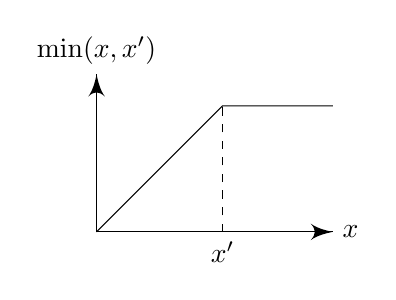
\begin{tikzpicture}
      \draw [->] (0, 0) -- (3, 0) node [right] {$x$};
      \draw [->] (0, 0) -- (0, 2) node [above] {$\min(x, x')$};

      \draw (0, 0) -- (1.6, 1.6) -- (3, 1.6);

      \draw [dashed] (1.6, 0) node [below] {$x'$} -- (1.6, 1.6);
    \end{tikzpicture}
  \end{center}
  Since we allow arbitrary linear combinations of these things and pointwise limits, this gives rise to a large class of functions. In particular, this includes all Lipschitz functions that are $0$ at the origin.

  In fact, the resulting space is a Sobolev space, with the norm given by% check this
  \[
    \|f\| = \left(\int_0^1 f'(x)^2 \;\d x \right)^{1/2}.
  \]
  For example, if we take $f = \min (\ph, x)$, then by definition we have
  \[
    \|\min(\ph, x)\|_\mathcal{H}^2 = \min(x, x) = x,
  \]
  whereas the formula we claimed gives
  \[
    \int_0^x 1^2 \;\d t = x.
  \]
\end{eg}

In general, it is difficult to understand the RKHS, but if we can do so, this provides a lot of information on what we are regularizing in the kernel trick.

\subsection{Making predictions}
Let's now try to understand what exactly we are doing when we do ridge regression with a kernel $k$. To do so, we first think carefully what we were doing in ordinary ridge regression, which corresponds to using the linear kernel. For the linear kernel, the $L^2$ norm $\|\beta\|_2^2$ corresponds exactly to the norm in the RKHS $\|f\|_{\mathcal{H}}^2$. Thus, an alternative way of expressing ridge regression is
\[
  \hat{f} = \argmin_{f \in \mathcal{H}} \left\{\sum_{i = 1}^n (Y_i - f(x_i))^2 + \lambda \|f\|_{\mathcal{H}}^2 \right\},\tag{$*$}
\]
where $\mathcal{H}$ is the RKHS of the linear kernel. Now this way of writing ridge regression makes sense for an arbitrary RKHS, so we might think this is what we should solve in general.

But if $\mathcal{H}$ is infinite dimensional, then naively, it would be quite difficult to solve $(*)$. The solution is provided by the representer theorem.

\begin{thm}[Representer theorem]\index{representer theorem}
  Let $\mathcal{H}$ be an RKHS with reproducing kernel $k$. Let $c$ be an arbitrary loss function and $J: [0, \infty) \to \R$ any strictly increasing function. Then the minimizer $\hat{f} \in \mathcal{H}$ of
  \[
    Q_1(f) = c(Y, x_1, \ldots, x_n, f(x_1), \ldots, f(x_n)) + J(\|f\|_{\mathcal{H}}^2)
  \]
  lies in the linear span of $\{k(\ph, x_i)\}_{i = 1}^n$.
\end{thm}

Given this theorem, we know our optimal solution can be written in the form
\[
  \hat{f}(\ph) = \sum_{i = 1}^n \hat{\alpha}_i k(\ph, x_i),
\]
and thus we can rewrite our optimization problem as looking for the $\hat{\alpha} \in \R^n$ that minimizes
\[
  Q_2(\alpha) = c(Y, x_1, \ldots, x_n, K\alpha) + J(\alpha^T K \alpha),
\]
over $\alpha \in \R^n$ (with $K_{ij} = k(x_i, x_j)$).

For an arbitrary $c$, this can still be quite difficult, but in the case of Ridge regression, this tells us that $(*)$ is equivalent to minimizing
\[
  \|Y - K\alpha\|_2^2 + \lambda \alpha^T K \alpha,
\]
and by differentiating, we find that this is given by solving
\[
  K \hat{\alpha} = K(K + \lambda I)^{-1} Y.
\]
Of course $K\hat{\alpha}$ is also our fitted values, so we see that if we try to minimize $(*)$, then the fitted values is indeed given by $K(K + \lambda I)^{-1}Y$, as in our original motivation.

\begin{proof}
  Suppose $\hat{f}$ minimizes $Q_1$. We can then write
  \[
    \hat{f} = u + v
  \]
  where $u \in V = \spn\{k(\ph, x_i): i = 1, \ldots ,n\}$ and $v \in V^\perp$. Then
  \[
    \hat{f}(x_i) = \bra f, k(\ph, x_i)\ket = \bra u + v, k(\ph, x_i)\ket = \bra u, k(\ph, x_i)\ket = u(x_i).
  \]
  So we know that
  \[
    c(Y, x_1, \ldots, x_n, f(x_1), \ldots, f(x_n)) = c(Y, x_1, \ldots, x_n, u(x_1), \ldots, u(x_n)).
  \]
  Meanwhile,
  \[
    \|f\|^2_{\mathcal{H}} = \|u + v\|^2_{\mathcal{H}} = \|u\|^2_{\mathcal{H}} + \|v\|^2_{\mathcal{H}},
  \]
  using the fact that $u$ and $v$ are orthogonal. So we know
  \[
    J(\|f\|_{\mathcal{H}}^2 ) \geq J(\|u\|_{\mathcal{H}}^2)
  \]
  with equality iff $v = 0$. Hence $Q_1(f) \geq Q_1(u)$ with equality iff $v = 0$, and so we must have $v = 0$ by optimality.

  Thus, we know that the optimizer in fact lies in $V$, and then the formula of $Q_2$ just expresses $Q_1$ in terms of $\alpha$.
\end{proof}

How well does our kernel machine do? Let $\mathcal{H}$ be an RKHS with reproducing kernel $k$, and $f^0 \in \mathcal{H}$. Consider a model
\[
  Y_i = f^0(x_i) + \varepsilon_i
\]
for $i = 1, \ldots, n$, and assume $\E \varepsilon = 0$, $\var(\varepsilon) = \sigma^2 I$.

For convenience, We assume $\|f^0\|^2_{\mathcal{H}} \leq 1$. There is no loss in generality by assuming this, since we can always achieve this by scaling the norm.

Let $K$ be the kernel matrix $K_{ij} = k(x_i, x_j)$ with eigenvalues $d_1 \geq d_2 \geq \cdots \geq d_n \geq 0$. Define
\[
  \hat{f}_\lambda = \argmin_{f \in \mathcal{H}} \left\{ \sum_{i = 1}^n (Y_i - f(x_i))^2 + \lambda \|f\|_\mathcal{H}^2\right\}.
\]
\begin{thm}
  We have
  \begin{align*}
    \frac{1}{n} \sum_{i = 1}^n \E(f^0(x_i) - \hat{f}_\lambda (x_i))^2 &\leq \frac{\sigma^2}{n} \sum_{i = 1}^n \frac{d_i^2}{(d_i + \lambda)^2} + \frac{\lambda}{4n}\\
    &\leq \frac{\sigma^2}{n} \frac{1}{\lambda} \sum_{i = 1}^n \min \left(\frac{d_i}{4}, \lambda\right) + \frac{\lambda}{4n}.
  \end{align*}
\end{thm}
Given a data set, we can compute the eigenvalues $d_i$, and thus we can compute this error bound.

\begin{proof}
  We know from the representer theorem that
  \[
    (\hat{f}_\lambda (x_i), \ldots, \hat{f}_\lambda (x_n))^T = K(K + \lambda I)^{-1} Y.
  \]
  Also, there is some $\alpha \in \R^n$ such that
  \[
    (f^0(x_1), \ldots, f^0(x_n))^T = K \alpha.
  \]
  Moreover, on the example sheet, we show that
  \[
    1 \geq \|f^0\|_{\mathcal{H}}^2 \geq \alpha^T K \alpha.
  \]
  Consider the eigen-decomposition $K = UDU^T$, where $U$ is orthogonal, $D_{ii} = d_i$ and $D_{ij} = 0$ for $i \not= j$. Then we have
  \begin{align*}
    \E \sum_{i = 1}^n (f^0(x_i) - \hat{f}_\lambda (x_i))^2 &= \E\|K\alpha - K(K + \lambda I)^{-1} (K\alpha + \varepsilon)\|_2^2\\
    \intertext{Noting that $K\alpha= (K + \lambda I)(K + \lambda I)^{-1} K\alpha$, we obtain}
    &= \E \norm{\lambda (K + \lambda I)^{-1} K\alpha - K(K + \lambda I)^{-1} \varepsilon}_2^2\\
    &= \underbrace{\lambda^2 \norm{(K + \lambda I)^{-1} K\alpha}_2^2}_{\mathrm{(I)}} + \underbrace{\E \norm{K(K + \lambda I)^{-1} \varepsilon}_2^2}_{\mathrm{(II)}}.
  \end{align*}
  At this stage, we can throw in the eigen-decomposition of $K$ to write (I) as
  \begin{align*}
    \mathrm{(I)} &= \lambda^2 \norm{(UDU^T + \lambda I)^{-1} UDU^T \alpha }_2^2\\
    &= \lambda^2 \|U (D + \lambda I)^{-1} \underbrace{D U^T \alpha}_{\theta} \|_2^2\\
    &= \sum_{i = 1}^n \theta_i^2 \frac{\lambda^2}{(d_i + \lambda)^2}
  \end{align*}
  Now we have
  \[
    \alpha^T K \alpha = \alpha^T U DU^T \alpha = \alpha^T U DD^+ DU^T,
  \]
  where $D^+$ is diagonal and
  \[
    D_{ii}^+ =
    \begin{cases}
      d_i^{-1} & d_i > 0\\
      0 & \text{otherwise}
    \end{cases}.
  \]
  We can then write this as
  \[
    \alpha^T K \alpha = \sum_{d_i > 0} \frac{\theta_i^2}{d_i}.
  \]
  The key thing we know about this is that it is $\leq 1$.

  Note that by definition of $\theta_i$, we see that if $d_i = 0$, then $\theta_i = 0$. So we can write
  \[
    \mathrm{(II)} = \sum_{i: d_i \geq 0} \frac{\theta_i^2}{d_i} \frac{d_i \lambda^2}{(d_i + \lambda)^2} \leq \lambda \max_{i = 1, \ldots, n} \frac{d_i \lambda}{(d_i + \lambda)^2}
  \]
  by H\"older's inequality with $(p, q) = (1, \infty)$. Finally, use the inequality that
  \[
    (a + b)^2 \geq 4ab
  \]
  to see that we have
  \[
    \mathrm{(I)} \leq \frac{\lambda}{4}.
  \]
  So we are left with (II), which is a bit easier. Using the trace trick, we have
  \begin{align*}
    \mathrm{(II)} &= \E \varepsilon^T (K + \lambda I)^{-1} K^2 (K + \lambda I)^{-1} \varepsilon\\
    &= \E \tr \left(K (K + \lambda I)^{-1} \varepsilon \varepsilon^T (K + \lambda I)^{-1} K\right)\\
    &= \tr \left(K (K + \lambda I)^{-1} \E(\varepsilon \varepsilon^T) (K + \lambda I)^{-1} K\right)\\
    &= \sigma^2 \tr \left(K^2(K + \lambda I)^{-2}\right)\\
    &= \sigma^2 \tr \left(UD^2 U^T (UDU^T + \lambda I)^{-2}\right)\\
    &= \sigma^2 \tr \left(D^2 (D + \lambda I)^{-2}\right)\\
    &= \sigma^2 \sum_{i = 1}^n \frac{d_i^2}{(d_i + \lambda)^2}.
  \end{align*}
  Finally, writing $\frac{d_i^2}{(d_i + \lambda)^2} = \frac{d_i}{\lambda} \frac{d_i \lambda}{(d_i + \lambda)^2}$, we have
  \[
    \frac{d_i^2}{(d_i + \lambda)^2} \leq \min \left(1, \frac{d_i}{4 \lambda}\right),
  \]
  and we have the second bound.
\end{proof}
How can we interpret this? If we look at the formula, then we see that we can have good benefits if the $d_i$'s decay quickly, and the exact values of the $d_i$ depend only on the choice of $x_i$. So suppose the $x_i$ are random and idd and independent of $\varepsilon$. Then the entire analysis is still valid by conditioning on $x_1, \ldots, x_n$.

We define $\hat{\mu}_i = \frac{d_i}{n}$, and $\lambda_n = \frac{\lambda}{n}$. Then we can rewrite our result to say
\[
  \frac{1}{n} \E \sum_{i = 1}^n (f^0(x_i) - \hat{f}_\lambda (x_i))^2 \leq \frac{\sigma^2}{\lambda_n} \frac{1}{n} \sum_{i = 1}^n \E \min\left(\frac{\hat{\mu}_i}{4}, \lambda_n\right) + \frac{\lambda_n}{4} \equiv \E \delta_n(\lambda_n).
\]
We want to relate this more directly to the kernel somehow. Given a density $p(x)$ on $\mathcal{X}$, \term{Mercer's theorem} guarantees the following eigenexpansion
\[
  k(x, x') = \sum_{j = 1}^\infty \mu_j e_j(x) e_j(x'),
\]
where the eigenvalues $\mu_j$ and eigenfunctions $e_j$ obey
\[
  \mu_j e_j(x') = \int_{\mathcal{X}} k(x, x') e_j(x) p(x)\;\d x
\]
and
\[
  \int_{\mathcal{X}} e_k(x) e_j(x) p(x)\;\d x = \mathbf{1}_{j = k}.
\]
One can then show that
\[
  \frac{1}{n} \E \sum_{i = 1}^n \min \left(\frac{\hat{\mu}_i}{4}, \lambda_n\right) \leq \frac{1}{n} \sum_{i = 1}^\infty \min\left(\frac{\mu_i}{4}, \lambda_n\right)
\]
up to some absolute constant factors. For a particular density $p(x)$ of the input space, we can try to solve the integral equation to figure out what the $\mu_j$'s are, and we can find the expected bound.

When $k$ is the Sobolev kernel and $p(x)$ is the uniform density, then it turns out we have
\[
  \frac{\mu_j}{4} = \frac{1}{\pi^2(2j - 1)^2}.
\]
By drawing a picture, we see that we can bound $\sum_{i = 1}^\infty \min \left(\frac{\mu_i}{4} , \lambda_n\right)$ by
\[
  \sum_{i = 1}^\infty \min \left(\frac{\mu_i}{4} , \lambda_n\right) \leq \int_0^\infty \lambda_n \wedge \frac{1}{\pi^2(2j - 1)^2}\;\d j \leq \frac{\sqrt{\lambda_n}}{\pi} + \frac{\lambda_n}{2}.
\]
So we find that
\[
  \E(\delta_n(\lambda_n)) = O \left(\frac{\sigma^2}{n \lambda_n^{1/2}} + \lambda_n\right).
\]
We can then find the $\lambda_n$ that minimizes this, and we see that we should pick
\[
  \lambda_n \sim \left(\frac{\sigma^2}{n}\right)^{2/3},
\]
which gives an error rate of $\sim \left(\frac{\sigma^2}{n}\right)^{2/3}$.

\subsection{Other kernel machines}
Recall that the representer theorem was much more general than what we used it for. We could apply it to any loss function. In particular, we can apply it to classification problems. For example, we might want to predict whether an email is a spam. In this case, we have $Y \in \{-1, 1\}^n$.

Suppose we are trying to find a hyperplane that separates the two sets $\{x_i\}_{y_i = 1}$ and $\{x_i\}_{i: Y_i = -1}$. Consider the really optimistic case where they can indeed be completely separated by a hyperplane through the origin. So there exists $\beta \in \R^p$ (the normal vector) with $y_i x_I^T \beta> 0$ for all $i$. Moreover, it would be nice if we can maximize the minimum distance between any of the points and the hyperplane defined by $\beta$. This is given by
\[
  \max \frac{y_i x_i^T \beta}{\|\beta\|_2}.
\]
Thus, we can formulate our problem as
\begin{center}
  maximize $M$ among $\beta \in \R^p, M \geq 0$ subject to $\frac{y_i x_i^T \beta}{\|\beta\|_2} \geq M$.
\end{center}

This optimization problem gives the hyperplane that maximizes the \emph{margin} between the two classes.

Let's think about the more realistic case where we cannot completely separate the two sets. We then want to impose a penalty for each point on the wrong side, and attempt to minimize the distance.

There are two options. We can use the penalty
\[
  \lambda \sum_{i = 1}^n \left(M - \frac{Y_i x_i^T \beta}{\|\beta\|_2}\right)_+
\]
where $t_+ = t \mathbf{1}_{t \geq 0}$. Another option is to take
\[
  \lambda \sum_{i = 1}^n \left(1 - \frac{Y_i x_i^T \beta}{M \|\beta\|_2}\right)_+
\]
which is perhaps more natural, since now everything is ``dimensionless''. We will actually use neither, but will start with the second form and massage it to something that can be attacked with our existing machinery. Starting with the second option, we can write our optimization problem as
\[
  \max_{M \geq 0, \beta \in \R^p} \left(M - \lambda \sum_{i = 1}^n \left(1 - \frac{Y_i x_i^T \beta}{M \|\beta\|_2}\right)_+\right).
\]
Since the objective function is invariant to any positive scaling of $\beta$, we may assume $\|\beta\|_2 = \frac{1}{M}$, and rewrite this problem as maximizing
\[
  \frac{1}{\|\beta\|_2} - \lambda \sum_{i = 1}^n (1 - Y_i x_i^T \beta)_+.
\]
Replacing $\max \frac{1}{\|\beta\|_2}$ with minimizing $\|\beta\|_2^2$ and adding instead of subtracting the penalty part, we modify this to say
\[
  \min_{\beta \in \R^p} \left(\|\beta\|_2^2 + \lambda \sum_{i = 1}^n (1 - Y_i x_i^T \beta)_+\right).
\]
The final change we make is that we replace $\lambda$ with $\frac{1}{\lambda}$, and multiply the whole equation by $\lambda$ to get
\[
  \min_{\beta \in \R^p} \left(\lambda \|\beta\|_2^2 + \sum_{i = 1}^n (1 - Y_i x_i^T \beta)_+\right).
\]
This looks much more like what we've seen before, with $\lambda \|\beta\|_2^2$ being the penalty term and $\sum_{i = 1}^n (1 - Y_i x_i^T \beta)_+$ being the loss function.

The final modification is that we want to allow planes that don't necessarily pass through the origin. To do this, we allow ourselves to translate all the $x_i$'s by a fixed vector $\delta \in \R^p$. This gives
\[
  \min_{\beta \in \R^p, \delta \in \R^p} \left(\lambda \|\beta\|_2^2 + \sum_{i = 1}^n \left(1 - Y_i (x_i - \delta)^T \beta\right)_+\right)
\]
Since $\delta^T \beta$ always appears together, we can simply replace it with a constant $\mu$, and write our problem as
\[
  (\hat{\mu}, \hat{\beta}) = \argmin_{(\mu, \beta) \in \R \times \R^p} \sum_{i = 1}^n \left(1 - Y_i (x_i^T \beta + \mu)\right)_+ + \lambda \|\beta\|_2^2.\tag{$*$}
\]
This gives the \term{support vector classifier}.

This is still just fitting a hyperplane. Now we would like to ``kernelize'' this, so that we can fit in a surface instead. Let $\mathcal{H}$ be the RKHS corresponding to the linear kernel. We can then write $(*)$ as
\[
  (\hat{\mu}_\lambda, \hat{f}_\lambda) = \argmin_{(\mu, f) \in \R \times \mathcal{H}} \sum_{i = 1}^n (1 - Y_i( f(x_i) + \mu))_+ + \lambda \|f\|_{\mathcal{H}}^2.
\]
The representer theorem (or rather, a slight variant of it) tells us that the above optimization problem is equivalent to the \term{support vector machine}
\[
  (\hat{\mu}_\lambda, \hat{\alpha}_\lambda) = \argmin_{(\mu, \alpha) \in \R \times \R^n}\sum_{i = 1}^n (1 - Y_i (K_i^T \alpha + \mu))_+ + \lambda \alpha^T K \alpha
\]
where $K_{ij} = k(x_i, x_j)$ and $k$ is the reproducing kernel of $\mathcal{H}$. Predictions at a new $x$ are then given by
\[
  \mathrm{sign} \left(\hat{\mu}_\lambda + \sum_{i = 1}^n \hat{\alpha}_{\lambda, i} k(x, x_i)\right).
\]

One possible alternative to this is to use \term{logistic regression}. Suppose that
\[
  \log \left(\frac{\P(Y_i = 1)}{\P(Y_i = -1)}\right) = x_i^T \beta^0,
\]
and that $Y_1, \ldots, Y_n$ are independent. An estimate of $\beta^0$ can be obtained through maximizing the likelihood, or equivalently,
\[
  \argmin_{~b \in \R^p} \sum_{i = 1}^n \log (1 + \exp(-Y_i x_i^T \beta)).
\]
To kernelize this, we introduce an error term of $\lambda \|\beta\|_2^2$, and then kernelize this. The resulting optimization problem is then given by
\[
  \argmin_{f \in \mathcal{H}} \left( \sum_{i = 1}^n \log (1 + \exp (-Y_i f(x_i))) + \lambda \|f\|_{\mathcal{H}}^2\right).
\]
We can then solve this using the representer theorem.

\subsection{Large-scale kernel machines}
How do we apply kernel machines at large scale? Whenever we want to make a prediction with a kernel machine, we need $O(n)$ many steps, which is quite a pain if we work with a large data set, say a few million of them. But even before that, forming $K \in \R^{n \times n}$ and inverting $K + \lambda I$ or equivalent can be computationally too expensive.

One of the more popular approaches to tackle these difficulties is to form a randomized feature map $\hat{\phi}: \mathcal{X} \to \R^b$ such that
\[
  \E \hat{\phi}(x)^T \hat{\phi}(x') = k(x, x')
\]
To increase the quality of the approximation, we can use
\[
  x \mapsto \frac{1}{\sqrt{L}}(\hat{\phi}_1(x), \ldots, \hat{\phi}_L(x))^T \in \R^{Lb},
\]
where the $\hat{\phi}_i(x)$ are iid with the same distribution as $\hat{\phi}$.

Let $\Phi$ be the matrix with $i$th row $\frac{1}{\sqrt{L}}(\hat{\phi}_1(x), \ldots, \hat{\phi}_L(x))$. When performing, e.g.\ kernel ridge regression, we can compute
\[
  \hat{\theta} = (\Phi^T \Phi + \lambda I)^{-1} \Phi^T Y.
\]
The computational cost of this is $O((Lb)^3 + n (Lb)^2)$. The key thing of course is that this is linear in $n$, and we can choose the size of $L$ so that we have a good trade-off between the computational cost and the accuracy of the approximation.

Now to predict a new $x$, we form
\[
  \frac{1}{\sqrt{L}} (\hat{\phi}_1(x), \ldots, \hat{\phi}_L(x))^T \hat{\theta},
\]
and this is $O(Lb)$.

In 2007, Rahimi and Recht proposed a random map for shift-invariant kernels, i.e.\ kernels $k$ such that $k(x, x') = h(x - x')$ for some $h$ (we work with $\mathcal{X} = \R^p$). A common example is the Gaussian kernel.

One motivation of this comes from a classical result known as \emph{Bochner's theorem}.

\begin{thm}[Bochner's theorem]\index{Bochner's theorem}
  Let $k: \R^p \times \R^p \to \R$ be a continuous kernel. Then $k$ is shift-invariant if and only if there exists some distribution $F$ on $\R^p$ and $c > 0$ such that if $W \sim F$, then
  \[
    k(x, x') = c\E \cos((x - x')^T W).
  \]
\end{thm}
Our strategy is then to find some $\hat{\phi}$ depending on $W$ such that
\[
  c\cos((x - x')^T W) = \hat{\phi}(x) \hat{\phi}(x').
\]
We are going to take $b = 1$, so we don't need a transpose on the right.

The idea is then to play around with trigonometric identities to try to write $c \cos ((x - x')^T W)$. After some work, we find the following solution:

Let $u \sim U[-\pi, \pi]$, and take $x, y \in \R$. Then
\[
  \E \cos(x + u)\cos (y + u) = \E (\cos x \cos u - \sin x \sin u)(\cos y \cos u - \sin y \sin u)
\]
Since $u$ has the same distribution as $-u$, we see that $\E \cos u\sin u = 0$.

Also, $\cos^2 u + \sin^2 u = 1$. Since $u$ ranges uniformly in $[-\pi, \pi]$, by symmetry, we have $\E \cos^2 u = \E \sin^2 u = \frac{1}{2}$. So we find that
\[
  2 \E \cos(x + u) \cos (y + u) = (\cos x \cos y + \sin x \sin y) = \cos (x - y).
\]
Thus, given a shift-invariant kernel $k$ with associated distribution $F$, we set $W \sim F$ independently of $u$. Define
\[
  \hat{\phi}(x) = \sqrt{2c} \cos (W^T x + u).
\]
Then
\begin{align*}
  \E \hat{\phi}(x) \hat{\phi}(x') &= 2c \E[\E[\cos (W^T x + u) \cos (W^T x' + u) \mid W]]\\
  &= c \E \cos(W^T (x - x'))\\
  &= k(x, x').
\end{align*}

In order to get this to work, we must find the appropriate $W$. In certain cases, this $W$ is actually not too hard to find:
\begin{eg}
  Take
  \[
    k(x, x') = \exp\left(-\frac{1}{2\sigma^2} \|x - x'\|_2^2\right),
  \]
  the Gaussian kernel. If $W \sim N(0, \sigma^{-2} I)$, then
  \[
    \E e^{it^TW} = e^{-\|t\|_2^2/(2\sigma^2)} = \E \cos(t^2 W).
  \]
\end{eg}

\section{The Lasso and beyond}
We are interested in the situation where we have a very large number of variables compared to the size of the data set. For example the data set might be all the genetic and environmental information about patients, and we want to predict if they have diabetes. The key property is that we expect that most of the data are not useful, and we want to select a small subset of variables that are relevant, and form prediction models based on them.

In these cases, ordinary least squares is not a very good tool. If there are more variables than the number of data points, then it is likely that we can pick the regression coefficients so that our model fits our data exactly, but this model is likely to be spurious, since we are fine-tuning our model based on the random fluctuations of a large number of irrelevant variables. Thus, we want to find a regression method that penalizes non-zero coefficients. Note that Ridge regression is not good enough --- it encourages small coefficients, but since it uses the $\ell_2$ norm, it's quite lenient towards small, non-zero coefficients, as the square of a small number is really small.

There is another reason to favour models that sets a lot of coefficients to zero. Consider the linear model
\[
  Y = X \beta^0 + \varepsilon,
\]
where as usual $\E \varepsilon = 0$ and $\var(\varepsilon) = \sigma^2 I$. Let $S = \{k : \beta^0_k \not= 0\}$, and let $s = |S|$. As before, we suppose we have some a priori belief that $s \ll p$.

For the purposes of this investigation, suppose $X$ has full column rank, so that we can use ordinary least squares. Then the prediction error is
\begin{align*}
  \frac{1}{n} \E \|X \beta^0 - X \hat{\beta}^{OLS} \|_2^2 &= \frac{1}{n} \E (\hat{\beta}^{OLS} - \beta^0)^T X^T X (\hat{\beta}^{OLS} - \beta^0)\\
  &= \frac{1}{n} \E \tr (\hat{\beta}^{OLS} - \beta^0) (\hat{\beta}^{OLS} - \beta^0)^T X^T X\\
  &= \frac{1}{n} \tr \E(\hat{\beta}^{OLS} - \beta^0) (\hat{\beta}^{OLS} - \beta^0)^T X^T X\\
  &= \frac{1}{n} \tr \E \sigma^2 (X^T X)^{-1} X^T X\\
  &= \sigma^2 \frac{p}{n}.
\end{align*}
Note that this does not depend on what $\beta^0$ is, but only on $\sigma^2, p$ and $n$.

In the situation we are interested in, we expect $s \ll p$. So if we can find $S$ and find ordinary least squares just on these, then we would have a mean squared prediction error of $\sigma^2 \frac{s}{n}$, which would be much much smaller.

We first discuss a few classical model methods that does this.

The first approach we may think of is the \emph{best subsets method}, where we try to do regression on all possible choices of $S$ and see which is the ``best''. For any set $M$ of indices, we let $X_M$ be the submatrix of $X$ formed from the columns of $X$ with index in $M$. We then regress $Y$ on $X_M$ for every $M \subseteq \{1, \ldots, p\}$, and then pick the best model via cross-validation, for example. A big problem with this is that the number of subsets grows exponentially with $p$, and so becomes infeasible for, say, $p > 50$.

Another method might be \emph{forward selection}. We start with an intercept-only model, and then add to the existing model the predictor that reduces the RSS the most, and then keep doing this until a fixed number of predictors have been added. This is quite a nice approach, and is computationally quite fast even if $p$ is large. However, this method is greedy, and if we make a mistake at the beginning, then the method blows up. In general, this method is rather unstable, and is not great from a practical perspective.

\subsection{The Lasso estimator}
The Lasso (Tibshirani, 1996) is a seemingly small modification of Ridge regression that solves our problems. It solves
\[
  (\hat{\mu}_\lambda^L, \hat{\beta}_\lambda^L) = \argmin_{(\mu, \beta) \in \R \times \R^p} \frac{1}{2n} \|Y - \mu 1 - X \beta\|_2^2 + \lambda \|\beta\|_1.
\]
The key difference is that we use an $\ell_1$ norm on $\beta$ rather than the $\ell_2$ norm,
\[
  \|\beta\|_1 = \sum_{k = 1}^p |\beta_k|.
\]
This makes it drastically different from Ridge regression. We will see that for $\lambda$ large, it will make all of the entries of $\beta$ exactly zero, as opposed to being very close to zero.

We can compare this to best subset regression, where we replace $\|\beta\|_1$ with something of the form $\sum_{k = 1}^p \mathbf{1}_{\beta_k > 0}$. But the beautiful property of the Lasso is that the optimization problem is now continuous, and in fact convex. This allows us to solve it using standard convex optimization techniques.

Why is the $\ell_1$ norm so different from the $\ell_2$ norm? Just as in Ridge regression, we may center and scale $X$, and center $Y$, so that we can remove $\mu$ from the objective. Define
\[
  Q_\lambda(\beta) = \frac{1}{2n} \|Y - X \beta\|_2^2 + \lambda \|\beta\|_1.
\]
Any minimizer $\hat{\beta}^L_\lambda$ of $Q_\lambda(\beta)$ must also be a solution to
\[
  \min \|Y - X \beta\|_2^2 \text{ subject to } \|\beta\|_1 \leq \|\hat{\beta}_\lambda^L\|_1.
\]
Similarly, $\hat{\beta}_\lambda^R$ is a solution of
\[
  \min \|Y - X \beta\|_2^2 \text{ subject to } \|\beta\|_2 \leq \|\hat{\beta}_\lambda^R\|_2.
\]
So imagine we are given a value of $\|\hat{\beta}_\lambda^L\|_1$, and we try to solve the above optimization problem with pictures. The region $\|\beta\|_1 \leq \|\hat{\beta}_\lambda^L\|_1$ is given by a rotated square
\begin{center}
  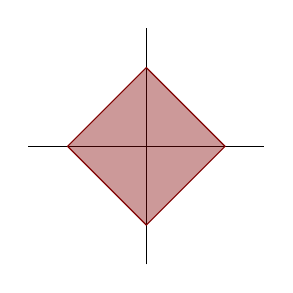
\begin{tikzpicture}
    \draw (-1.5, 0) -- (1.5, 0);
    \draw (0, -1.5) -- (0, 1.5);

    \draw [mred, fill, fill opacity=0.4] (1, 0) -- (0, 1) -- (-1, 0) -- (0, -1) -- cycle;
  \end{tikzpicture}
\end{center}
On the other hand, the minimum of $\|Y - X \beta\|_2^2$ is at $\hat{\beta}^{OLS}$, and the contours are ellipses centered around this point.
\begin{center}
  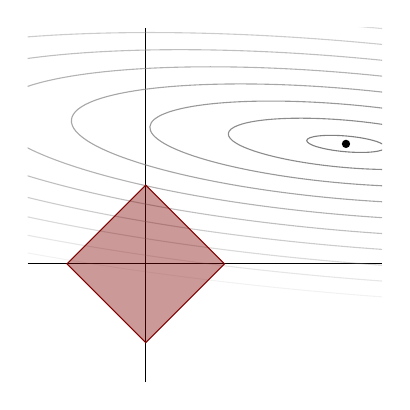
\begin{tikzpicture}
    \clip (-1.5, -1.5) rectangle (3, 3);
    \draw (-1.5, 0) -- (3, 0);
    \draw (0, -1.5) -- (0, 3);

    \begin{scope}[rotate=-5, shift={(2.4, 1.74)}]
      \node [circ] {};
      \draw [gray] ellipse (0.5 and 0.1);
      \draw [gray, opacity=0.9] ellipse (1.5 and 0.3);
      \draw [gray, opacity=0.8] ellipse (2.5 and 0.5);
      \draw [gray, opacity=0.7] ellipse (3.5 and 0.7);
      \draw [gray, opacity=0.6] ellipse (4.5 and 0.9);
      \draw [gray, opacity=0.5] ellipse (5.5 and 1.1);
      \draw [gray, opacity=0.4] ellipse (6.5 and 1.3);
      \draw [gray, opacity=0.3] ellipse (7.5 and 1.5);
      \draw [gray, opacity=0.2] ellipse (8.5 and 1.7);
      \draw [gray, opacity=0.1] ellipse (9.5 and 1.9);
    \end{scope}
    \draw [mred, fill, fill opacity=0.4] (1, 0) -- (0, 1) -- (-1, 0) -- (0, -1) -- cycle;
  \end{tikzpicture}
\end{center}
To solve the minimization problem, we should pick the smallest contour that hits the square, and pick the intersection point to be our estimate of $\beta^0$. The point is that since the unit ball in the $\ell^1$-norm has these corners, this $\beta^0$ is likely to be on the corners, hence has a lot of zeroes. Compare this to the case of Ridge regression, where the constraint set is a ball:
\begin{center}
  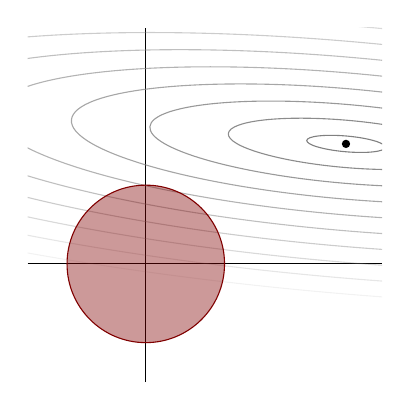
\begin{tikzpicture}
    \clip (-1.5, -1.5) rectangle (3, 3);
    \draw (-1.5, 0) -- (3, 0);
    \draw (0, -1.5) -- (0, 3);

    \begin{scope}[rotate=-5, shift={(2.4, 1.74)}]
      \node [circ] {};
      \draw [gray] ellipse (0.5 and 0.1);
      \draw [gray, opacity=0.9] ellipse (1.5 and 0.3);
      \draw [gray, opacity=0.8] ellipse (2.5 and 0.5);
      \draw [gray, opacity=0.7] ellipse (3.5 and 0.7);
      \draw [gray, opacity=0.6] ellipse (4.5 and 0.9);
      \draw [gray, opacity=0.5] ellipse (5.5 and 1.1);
      \draw [gray, opacity=0.4] ellipse (6.5 and 1.3);
      \draw [gray, opacity=0.3] ellipse (7.5 and 1.5);
      \draw [gray, opacity=0.2] ellipse (8.5 and 1.7);
      \draw [gray, opacity=0.1] ellipse (9.5 and 1.9);
    \end{scope}
    \draw [mred, fill, fill opacity=0.4] circle [radius=1];
  \end{tikzpicture}
\end{center}
Generically, for Ridge regression, we would expect the solution to be non-zero everywhere.

More generally, we can try to use the $\ell_q$ norm given by
\[
  \|\beta\|_q = \left(\sum_{k = 1}^p \beta_k^q\right)^{1/q}.
\]
We can plot their unit spheres, and see that they look like

\begin{center}
  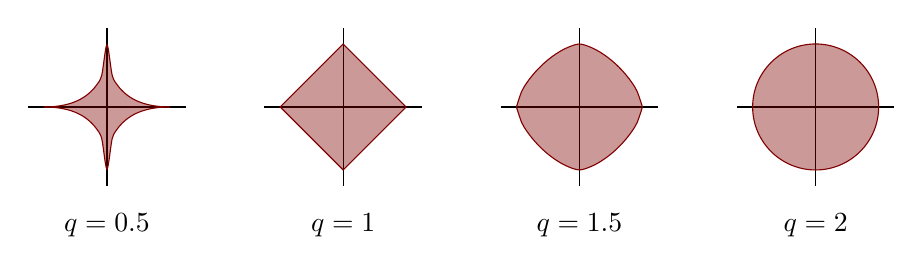
\begin{tikzpicture}
    \begin{scope}[shift={(0, 0)}]
      \draw (-1, 0) -- (1, 0);
      \draw (0, -1) -- (0, 1);
      \draw [domain=-0.8:0.8, mred, fill, fill opacity=0.4] plot [smooth] (\x, {(0.8^0.5 - (abs(\x))^0.5)^2});
      \draw [domain=-0.8:0.8, mred, fill, fill opacity=0.4] plot [smooth] (\x, {-(0.8^0.5 - (abs(\x))^0.5)^2});

      \node at (0, -1.5) {$q = 0.5$};
    \end{scope}
    \begin{scope}[shift={(3, 0)}]
      \draw (-1, 0) -- (1, 0);
      \draw (0, -1) -- (0, 1);
      \draw [mred, fill, fill opacity=0.4] (0.8, 0) -- (0, 0.8) -- (-0.8, 0) -- (0, -0.8) -- cycle;

      \node at (0, -1.5) {$q = 1$};
    \end{scope}
    \begin{scope}[shift={(6, 0)}]
      \draw (-1, 0) -- (1, 0);
      \draw (0, -1) -- (0, 1);
      \draw [domain=-0.8:0.8, mred, fill, fill opacity=0.4] plot [smooth] (\x, {(0.8^1.5 - (abs(\x))^1.5)^(1/1.5)});
      \draw [domain=-0.8:0.8, mred, fill, fill opacity=0.4] plot [smooth] (\x, {-(0.8^1.5 - (abs(\x))^1.5)^(1/1.5)});

      \node at (0, -1.5) {$q = 1.5$};
    \end{scope}
    \begin{scope}[shift={(9, 0)}]
      \draw (-1, 0) -- (1, 0);
      \draw (0, -1) -- (0, 1);
      \draw [mred, fill, fill opacity=0.4] circle [radius=0.8];

      \node at (0, -1.5) {$q = 2$};
    \end{scope}

  \end{tikzpicture}
\end{center}

We see that $q = 1$ is the smallest value of $q$ for which there are corners, and also the largest value of $q$ for which the constraint set is still convex. Thus, $q = 1$ is the sweet spot for doing regression.

But is this actually good? Suppose the columns of $X$ are scaled to have $\ell_2$ norm $\sqrt{n}$, and, after centering, we have a normal linear model
\[
  Y = X \beta^0 + \varepsilon- \bar{\varepsilon} 1,
\]
with $\varepsilon \sim N_n(0, \sigma^2 I)$.

\begin{thm}
  Let $\hat{\beta}$ be the Lasso solution with
  \[
    \lambda = A \sigma \sqrt{\frac{\log p}{n}}
  \]
  for some $A$. Then with probability $1 - 2p^{-(A^2/2 - 1)}$, we have
  \[
    \frac{1}{n} \|X \beta^0 - X \hat{\beta}\|_2^2 \leq 4A \sigma \sqrt{\frac{\log p}{n}} \|\beta^0\|_1.
  \]
\end{thm}
Crucially, this is proportional to $\log p$, and not just $p$. On the other hand, unlike what we usually see for ordinary least squares, we have $\frac{1}{\sqrt{n}}$, and not $\frac{1}{n}$.

We will later obtain better bounds when we make some assumptions on the design matrix.

\begin{proof}
  We don't really have a closed form solution for $\hat{\beta}$, and in general it doesn't exist. So the only thing we can use is that it in fact minimizes $Q_\lambda(\beta)$. Thus, by definition, we have
  \[
    \frac{1}{2n} \|Y - X \hat{\beta}\|_2^2 + \lambda \|\hat{\beta}\|_1 \leq \frac{1}{2n} \|Y - X \beta^0\|^2_2 + \lambda \|\beta^0\|_1.
  \]
  We know exactly what $Y$ is. It is $X \beta^0 + \varepsilon - \bar{\varepsilon} 1$. If we plug this in, we get
  \[
    \frac{1}{2n} \|X \beta^0 - X \hat{\beta}\|_2^2 \leq \frac{1}{n} \varepsilon^T X(\hat{\beta} - \beta^0) + \lambda \|\beta^0\|_1 - \lambda \|\hat{\beta}\|_1.
  \]
  Here we use the fact that $X$ is centered, and so is orthogonal to $1$.

  Now H\"older tells us
  \[
    |\varepsilon^T X (\hat{\beta} - \beta^0)| \leq \|X^T \varepsilon \|_\infty \|\hat{\beta} - \beta^0\|_1.
  \]
  We'd like to bound $\|X^T \varepsilon \|_\infty$, but it can be arbitrarily large since $\varepsilon$ is a Gaussian. However, with high probability, it is small. Precisely, define
  \[
    \Omega = \left\{\frac{1}{n} \|X^T \varepsilon \|_\infty \leq \lambda\right\}.
  \]
  In a later lemma, we will show later that $\P(\Omega) \geq 1 - 2 p^{-(A^2/2 - 1)}$. Assuming $\Omega$ holds, we have
  \[
    \frac{1}{2n} \|X \beta^0 - X \hat{\beta}\|^2_2 \leq \lambda \|\hat{\beta} - \beta^0\| - \lambda \|\hat{\beta}\| + \lambda \|\beta^0\| \leq 2 \lambda \|\beta^0\|_1.\qedhere
  \]
\end{proof}

\subsection{Basic concentration inequalities}
We now have to prove the lemma we left out in the theorem just now. In this section, we are going to prove a bunch of useful inequalities that we will later use to prove bounds.

Consider the event $\Omega$ as defined before. Then
\begin{align*}
  \P\left(\frac{1}{n} \|X^T \varepsilon\|_\infty > \lambda\right) &= \P\left(\bigcup_{j = 1}^p \left\{\frac{1}{n}|X_j^T \varepsilon| > \lambda\right\}\right)\\
  &\leq \sum_{j = 1}^p \P\left(\frac{1}{n} |X_j^T \varepsilon| > \lambda\right).
\end{align*}
Now $\frac{1}{n} X_j^T \varepsilon \sim N(0, \frac{\sigma^2}{n})$. So we just have to bound tail probabilities of normal random variables.

The simplest tail bound we have is Markov's inequality.
\begin{lemma}[Markov's inequality]\index{Markov's inequality}
  Let $W$ be a non-negative random variable. Then
  \[
    \P(W \geq t) \leq \frac{1}{t} \E W.
  \]
\end{lemma}

\begin{proof}
  We have
  \[
    t \mathbf{1}_{W \geq t} \leq W.
  \]
  The result then follows from taking expectations and then dividing both sides by $t$.
\end{proof}

While this is a very simple bound, it is actually quite powerful, because it assumes almost nothing about $W$. This allows for the following trick: given any strictly increasing function $\varphi: \R \to (0, \infty)$ and any random variable $W$, we have
\[
  \P(W \geq t) = \P(\varphi(W) \geq \varphi(t))\leq \frac{\E \varphi(W)}{\varphi(t)}.
\]
So we get a bound on the tail probability of $W$ for \emph{any} such function. Even better, we can minimize the right hand side over a class of functions to get an even better bound.

In particular, applying this with $\varphi (t) = e^{\alpha t}$ gives
\begin{cor}[Chernoff bound]\index{Chernoff bound}
  For any random variable $W$, we have
  \[
    \P(W \geq t) \leq \inf_{\alpha > 0} e^{-\alpha t} \E e^{\alpha W}.
  \]
\end{cor}
Note that $\E e^{\alpha W}$ is just the \term{moment generating function} of $W$, which we can compute quite straightforwardly.

We can immediately apply this when $W$ is a normal random variable, $W \sim N(0, \sigma^2)$. Then
\[
  \E e^{\alpha W} = e^{\alpha^2 \sigma^2/2}.
\]
So we have
\[
  \P(W \geq t) \leq \inf_{\alpha > 0}\exp \left(\frac{\alpha^2 \sigma^2}{2} - \alpha t\right) = e^{-t^2/(2\sigma^2)}.
\]
Observe that in fact this tail bound works for any random variable whose moment generating function is bounded above by $e^{\alpha^2 \sigma^2/2}$.

\begin{defi}[Sub-Gaussian random variable]\index{sub-Gaussian random variable}
  A random variable $W$ is \emph{sub-Gaussian} (with parameter $\sigma$) if
  \[
    \E e^{\alpha (W - \E W)} \leq e^{\alpha^2 \sigma^2/2}
  \]
  for all $\alpha \in \R$.
\end{defi}

\begin{cor}
  Any sub-Gaussian random variable $W$ with parameter $\sigma$ satisfies
  \[
    \P(W \geq t) \leq e^{-t^2/2\sigma^2}.\tag*{$\square$}
  \]
\end{cor}

In general, bounded random variables are sub-Gaussian.
\begin{lemma}[Hoeffding's lemma]\index{Hoeffding's lemma}
  If $W$ has mean zero and takes values in $[a, b]$, then $W$ is sub-Gaussian with parameter $\frac{b - a}{2}$.\fakeqed
\end{lemma}

Recall that the sum of two independent Gaussians is still a Gaussian. This continues to hold for sub-Gaussian random variables.

\begin{prop}
  Let $(W_i)_{i = 1}^n$ be independent mean-zero sub-Gaussian random variables with parameters $(\sigma_i)_{i = 0}^n$, and let $\gamma \in \R^n$. Then $\gamma^T W$ is sub-Gaussian with parameter
  \[
    \left(\sum (\gamma_i \sigma_i)^2\right)^{1/2}.
  \]
\end{prop}

\begin{proof}
  We have
  \begin{align*}
    \E \exp \left(\alpha \sum_{i = 1}^n \gamma_i W_i\right) &= \prod_{i = 1}^n \E \exp \left(\alpha \gamma_i W_i\right)\\
    &\leq \prod_{i = 1}^n \exp\left(\frac{\alpha^2}{2} \gamma_i^2 \sigma_i^2\right)\\
    &= \exp\left(\frac{\alpha^2}{2} \sum_{i = 1}^n \sigma_i^2 \gamma_i^2\right).\qedhere
  \end{align*}
\end{proof}

We can now prove our bound for the Lasso, which in fact works for any sub-Gaussian random variable.
\begin{lemma}
  Suppose $(\varepsilon_i)_{i = 1}^n$ are independent, mean-zero sub-Gaussian with common parameter $\sigma$. Let
  \[
    \lambda = A \sigma \sqrt{\frac{\log p}{n}}.
  \]
  Let $X$ be a matrix whose columns all have norm $\sqrt{n}$. Then
  \[
    \P\left(\frac{1}{n} \|X^T \varepsilon\|_{\infty} \leq \lambda\right) \geq 1 - 2p^{-(A^2/2 - 1)}.
  \]
\end{lemma}
In particular, this includes $\varepsilon \sim N_n(0, \sigma^2I)$.

\begin{proof}
  We have
  \[
    \P\left(\frac{1}{n}\|X^T \varepsilon\|_{\infty} > \lambda \right) \leq \sum_{j = 1}^p \P\left(\frac{1}{n} |X_j^T \varepsilon| > \lambda\right).
  \]
  But $\pm \frac{1}{n} X_j^T \varepsilon$ are both sub-Gaussian with parameter
  \[
    \sigma \left(\sum_i \left(\frac{X_{ij}}{n}\right)^2\right)^{1/2} = \frac{\sigma}{\sqrt{n}}.
  \]
  Then by our previous corollary, we get
  \[
    \sum_{j = 1}^p \P\left(\frac{1}{n} |X_j^T \varepsilon|_\infty > \lambda\right) \leq 2p \exp \left(- \frac{\lambda^2 n}{2\sigma^2}\right).
  \]
  Note that we have the factor of $2$ since we need to consider the two cases $\frac{1}{n} X_j^T \varepsilon > \lambda$ and $-\frac{1}{n} X_j^T \varepsilon > \lambda$.

  Plugging in our expression of $\lambda$, we write the bound as
  \[
    2p \exp\left(-\frac{1}{2} A^2 \log p\right) = 2p^{1 - A^2/2}.\qedhere
  \]
\end{proof}
This is all we need for our result on the Lasso. We are going to go a bit further into this topic of concentration inequalities, because we will need them later when we impose conditions on the design matrix. In particular, we would like to bound the tail probabilities of products.

\begin{defi}[Bernstein's condition]\index{Bernstein's condition}
  We say that a random variable $W$ satisfies Bernstein's condition with parameters $(\sigma, b)$ where $a, b > 0$ if
  \[
    \E[|W - \E W|^k] \leq \frac{1}{2} k!\, \sigma^2 b^{k - 2}
  \]
  for $k = 2, 3, \ldots$.
\end{defi}
The point is that these bounds on the moments lets us bound the moment generating function of $W$.

\begin{prop}[Bernstein's inequality]\index{Bernstein's inequality}
  Let $W_1, W_2, \ldots, W_n$ be independent random variables with $\E W_i = \mu$, and suppose each $W_i$ satisfies Bernstein's condition with parameters $(\sigma, b)$. Then
  \begin{align*}
    \E e^{\alpha(W_i - \mu)} &\leq \exp \left(\frac{\alpha^2 \sigma^2/2}{1 - b|\alpha|}\right)\text{ for all }|\alpha| < \frac{1}{b},\\
    \P\left(\frac{1}{n} \sum_{i = 1}^n W_i - \mu \geq t\right) &\leq \exp \left(-\frac{nt^2}{2 (\sigma^2 + bt)}\right)\text{ for all } t \geq 0.
  \end{align*}
\end{prop}
Note that for large $t$, the bound goes as $e^{-t}$ instead of $e^{-t^2}$.

\begin{proof}
  For the first part, we fix $i$ and write $W = W_i$. Let $|\alpha| < \frac{1}{b}$. Then
  \begin{align*}
    \E e^{\alpha(W_i - \mu)} &= \sum_{k = 0}^\infty \E \left[\frac{1}{k!} \alpha^k |W_i - \mu|^k\right]\\
    &\leq 1 + \frac{\sigma^2 \alpha^2}{2} \sum_{k = 2}^\infty |\alpha|^{k - 2} b^{k - 2}\\
    &= 1 + \frac{\sigma^2 \alpha^2}{2} \frac{1}{1 - |\alpha|b}\\
    &\leq \exp \left(\frac{\alpha^2 \sigma^2/2}{1 - b|\alpha|}\right).
  \end{align*}
  Then
  \begin{align*}
    \E \exp\left(\frac{1}{n} \sum_{i = 1}^n \alpha (W_i - \mu)\right) &= \prod_{i = 1}^n \E \exp\left(\frac{\alpha}{n} (W_i - \mu)\right)\\
    &\leq \exp \left(n \frac{\left(\frac{\alpha}{n}\right)^2 \sigma^2/2}{1 - b \left|\frac{\alpha}{n}\right|}\right),
  \end{align*}
  assuming $\left|\frac{\alpha}{n}\right| < \frac{1}{b}$. So it follows that
  \[
    \P \left(\frac{1}{n} \sum_{i = 1}^n W_i - \mu \geq t\right) \leq e^{-\alpha t}\exp \left(n \frac{\left(\frac{\alpha}{n}\right)^2 \sigma^2/2}{1 - b \left|\frac{\alpha}{n}\right|}\right).
  \]
  Setting
  \[
    \frac{\alpha}{n} = \frac{t}{bt + \sigma^2} \in \left[0, \frac{1}{b}\right)
  \]
  gives the result.
\end{proof}

\begin{lemma}
  Let $W, Z$ be mean-zero sub-Gaussian random variables with parameters $\sigma_W$ and $\sigma_Z$ respectively. Then $WZ$ satisfies Bernstein's condition with parameter $(8 \sigma_W \sigma_Z, 4 \sigma_W \sigma_Z)$.
\end{lemma}

\begin{proof}
  For any random variable $Y$ (which we will later take to be $WZ$), for $k > 1$, we know
  \begin{align*}
    \E |Y - \E Y|^k &= 2^k \E \left| \frac{1}{2}Y - \frac{1}{2}\E Y\right|^k\\
    &\leq 2^k \E \left| \frac{1}{2} |Y| + \frac{1}{2} |\E Y|\right|^k.
  \end{align*}
  Note that
  \[
    \left| \frac{1}{2} |Y| + \frac{1}{2} |\E Y|\right|^k \leq \frac{|Y|^k + |\E Y|^k}{2}
  \]
  by Jensen's inequality. Applying Jensen's inequality again, we have
  \[
    |\E Y|^k \leq \E |Y|^k.
  \]
  Putting the whole thing together, we have
  \[
    \E |Y - \E Y|^k \leq 2^k \E |Y|^k.
  \]
  Now take $Y = WZ$. Then
  \[
    \E |WZ - \E WZ| \leq 2^k \E |WZ|^k \leq 2^k \left(\E W^{2k}\right)^{1/2} (\E Z^{2k})^{1/2},
  \]
  by the Cauchy--Schwarz inequality.

  We know that sub-Gaussians satisfy a bound on the tail probability. We can then use this to bound the moments of $W$ and $Z$. First note that
  \[
    W^{2k} = \int_0^\infty \mathbf{1}_{x < W^{2k}} \;\d x.
  \]
  Taking expectations of both sides, we get
  \[
    \E W^{2k} = \int_0^\infty \P(x < W^{2k})\;\d x.
  \]
  Since we have a tail bound on $W$ instead of $W^{2k}$, we substitute $x = t^{2k}$. Then $\d x = 2k t^{2k - 1}\;\d t$. So we get
  \begin{align*}
    \E W^{2k} &= 2k \int_0^\infty t^{2k - 1} \P(|W| > t) \;\d t\\
    &= 4k \int_0^\infty t^{2k} \exp \left(-\frac{t^2}{2 \sigma_N^2}\right)\;\d t.
  \end{align*}
  where again we have a factor of $2$ to account for both signs. We perform yet another substitution
  \[
    x = \frac{t^2}{2 \sigma_N^2},\quad \d x = \frac{t}{\sigma_W^2}\;\d t.
  \]
  Then we get
  \[
    \E W^{2k} = 2^{k + 1} \sigma_W^{2k} k \sigma_W^2 \int_0^\infty x^{k - 1} e^{-x}\;\d x = 4 \cdot k! \sigma_W^2.
  \]
  Plugging this back in, we have
  \begin{align*}
    \E|WZ - \E WZ|^k &\leq 2^k 2^{k + 1} k! \sigma_W^k \sigma_Z^k \sigma_Z^k\\
    &= \frac{1}{2} k! 2^{2k + 2} \sigma_W^k \sigma_Z^k\\
    &= \frac{1}{2} k! (8 \sigma_W \sigma_Z)^2 (4 \sigma_W \sigma_Z)^{k - 2}.\qedhere
  \end{align*}
\end{proof}

\subsection{Convex analysis and optimization theory}
We'll leave these estimates aside for a bit, and give more background on convex analysis and convex optimization. Recall the following definition:
\begin{defi}[Convex set]\index{convex set}
  A set $A \subseteq \R^d$ is convex if for any $x, y \in A$ and $t \in [0, 1]$, we have
  \[
    (1 - t)x + ty \in A.
  \]
\end{defi}
\begin{center}
  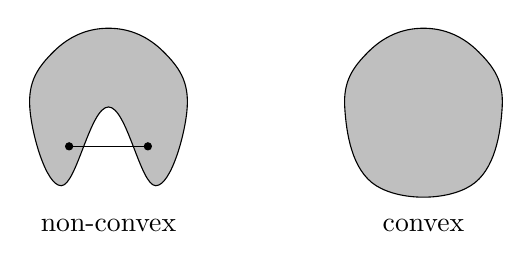
\begin{tikzpicture}
    \begin{scope}[shift={(-2, 0)}]
      \draw [fill=gray!50!white] plot [smooth cycle, tension=0.7] coordinates {(0, 1) (-0.7, 0.7) (-1, 0) (-0.6, -1) (0, 0) (0.6, -1) (1, 0) (0.7, 0.7)};
      \draw (-0.5, -0.5) node [circ] {} -- (0.5, -0.5) node [circ] {};

      \node at (0, -1.5) {non-convex};
    \end{scope}

    \begin{scope}[shift={(2, 0)}]
      \draw [fill=gray!50!white] plot [smooth cycle, tension=0.7] coordinates {(0, 1) (-0.7, 0.7) (-1, 0) (-0.6, -1) (0.6, -1) (1, 0) (0.7, 0.7)};
      \node at (0, -1.5) {convex};
    \end{scope}
  \end{tikzpicture}
\end{center}

We are actually more interested in convex functions. We shall let our functions to take value $\infty$, so let us define $\bar{\R} = \R \cup \{\infty\}$. The point is that if we want our function to be defined in $[a, b]$, then it is convenient to extend it to be defined on all of $\R$ by setting the function to be $\infty$ outside of $[a, b]$.

\begin{defi}[Convex function]\index{convex function}
  A function $f: \R^d \to \bar{\R}$ is \emph{convex} iff
  \[
    f((1 - t)x + ty) \leq (1 - t) f(x) + t f(y)
  \]
  for all $x, y \in \R^d$ and $t \in (0, 1)$. Moreover, we require that $f(x) < \infty$ for at least one $x$.

  We say it is \emph{strictly convex} if the inequality is strict for all $x, y$ and $t \in (0, 1)$.
\end{defi}
\begin{center}
  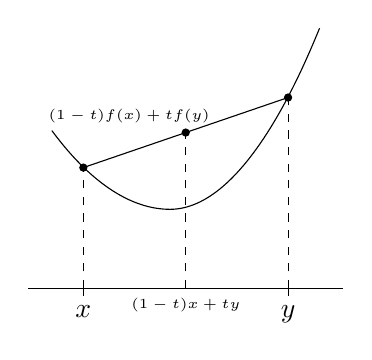
\begin{tikzpicture}
    \draw (-2, 0) -- (2, 0);
    \draw (-1.3, 0.1) -- (-1.3, -0.1) node [below] {$x$};
    \draw (1.3, 0.1) -- (1.3, -0.1) node [below] {$y$};
    \draw (-1.7, 2) parabola bend (-.2, 1) (1.7, 3.3);
    \draw [dashed] (-1.3, 0) -- (-1.3, 1.53) node [circ] {};
    \draw [dashed] (1.3, 0) -- (1.3, 2.42) node [circ] {};
    \draw (-1.3, 1.53) -- (1.3, 2.42);
    \draw [dashed] (0, 0) node [below] {\tiny $(1 - t) x + t y$} -- (0, 1.975) node [above] {\tiny$(1 - t) f(x) + t f(y)\quad\quad\quad\quad\quad\quad$} node [circ] {};
  \end{tikzpicture}
\end{center}

\begin{defi}[Domain]\index{domain}
  Define the \emph{domain} of a function $f: \R^d \to \bar{\R}$ to be
  \[
    \dom f = \{x : f(x) < \infty\}.
  \]
\end{defi}
One sees that the domain of a convex function is always convex.

\begin{prop}\leavevmode
  \begin{enumerate}
    \item Let $f_1, \ldots, f_m: \R^d \to \bar{\R}$ be convex with $\dom f_1 \cap \cdots \cap \dom f_m \not = \emptyset$, and let $c_1, \ldots, c_m \geq 0$. Then $c_1 + \cdots + c_m f_m$ is a convex function.
    \item If $f: \R^d \to \R$ is twice continuously differentiable, then
      \begin{enumerate}
        \item $f$ is convex iff its Hessian is positive semi-definite everywhere.
        \item $f$ is strictly convex if its Hessian positive definite everywhere.\fakeqed
      \end{enumerate}
  \end{enumerate}
\end{prop}
Note that having a positive definite Hessian is not necessary for strict convexity, e.g.\ $x^4$ is strictly convex but has vanishing Hessian at $0$.

Now consider a constrained optimization problem
\begin{center}
  minimize $f(x)$ subject to $g(x) = 0$
\end{center}
where $x \in \R^d$ and $g: \R^d \to \R^b$. The \term{Lagrangian} for this problem is
\[
  L(x, \theta) = f(x) + \theta^T g(x).
\]
Why is this helpful? Suppose $c^*$ is the minimum of $f$. Then note that for any $\theta$, we have
\[
  \inf_{x \in \R^d} L(x, \theta) \leq \inf_{x \in \R^d, g(x) = 0} L(x, \theta) = \inf_{x \in \R^d: g(x) = 0} f(x) = c^*.
\]
Thus, if we can find some $\theta^*, x^*$ such that $x^*$ minimizes $L(x, \theta^*)$ and $g(x^*) = 0$, then this is indeed the optimal solution.

This gives us a method to solve the optimization problem --- for each fixed $\theta$, solve the unconstrained optimization problem $\argmin_x L(x, \theta)$. If we are doing this analytically, then we would have a formula for $x$ in terms of $\theta$. Then seek for a $\theta$ such that $g(x) = 0$ holds.

\subsubsection*{Subgradients}
Usually, when we have a function to optimize, we take its derivative and set it to zero. This works well if our function is actually differentiable. However, the $\ell_1$ norm is not a differentiable function, since $|x|$ is not differentiable at $0$. This is not some exotic case we may hope to avoid most of the time --- when solving the Lasso, we actively want our solutions to have zeroes, so we really want to get to these non-differentiable points.

Thus, we seek some generalized notion of derivative that works on functions that are not differentiable.

\begin{defi}[Subgradient]\index{subgradient}
  A vector $v \in \R^d$ is a \emph{subgradient} of a convex function at $x$ if $f(y) \geq f(x) + v^T(y - x)$ for all $y \in \R^d$.

  The set of subgradients of $f$ at $x$ is denoted $\partial f(x)$, and is called the \term{subdifferential}.
\end{defi}
\begin{center}
  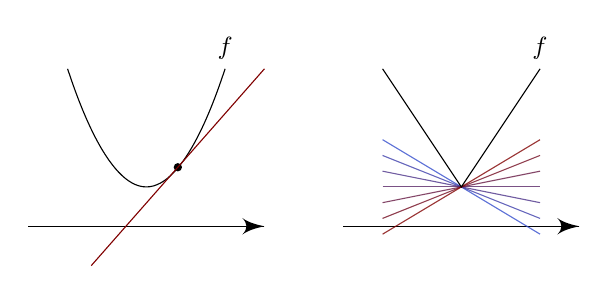
\begin{tikzpicture}
    \draw [->] (-1.5, -0.5) -- (1.5, -0.5);
    \draw (-1, 1.5) parabola bend (0, 0) (1, 1.5) node [above] {\small $f$};
    \node [circ] at (0.4, 0.25) {};
    \draw [mred] (-0.7, -1) -- (1.5, 1.5);

    \begin{scope}[shift={(4, 0)}]
      \draw [->] (-1.5, -0.5) -- (1.5, -0.5);

      \draw [opacity=0.8, mred!0!mblue] (-1, 0.6) -- (1, -0.6);
      \draw [opacity=0.8, mred!16!mblue] (-1, 0.4) -- (1, -0.4);
      \draw [opacity=0.8, mred!33!mblue] (-1, 0.2) -- (1, -0.2);
      \draw [opacity=0.8, mred!50!mblue] (-1, 0) -- (1, 0);
      \draw [opacity=0.8, mred!67!mblue] (-1, -0.2) -- (1, 0.2);
      \draw [opacity=0.8, mred!84!mblue] (-1, -0.4) -- (1, 0.4);
      \draw [opacity=0.8, mred!100!mblue] (-1, -0.6) -- (1, 0.6);

      \draw (-1, 1.5) -- (0, 0) -- (1, 1.5) node [above] {\small $f$};
    \end{scope}
  \end{tikzpicture}
\end{center}

This is indeed a generalization of the derivative, since
\begin{prop}
  Let $f$ be convex and differentiable at $x \in \mathrm{int}(\dom f)$. Then $\partial f(x) = \{\nabla f(x)\}$.\fakeqed
\end{prop}

The following properties are immediate from definition.
\begin{prop}
  Suppose $f$ and $g$ are convex with $\mathrm{int}(\dom f) \cap \mathrm{int} (\dom g) \not= \emptyset$, and $\alpha > 0$. Then
  \begin{align*}
    \partial (\alpha f)(x) &= \alpha \partial f(x) = \{\alpha v: v \in \partial f(x)\}\\
    \partial (f + g)(x) &= \partial g(x) + \partial f(x).\fakeqed
  \end{align*}
\end{prop}

The condition (for convex differentiable functions) that ``$x$ is a minimum iff $f'(x) = 0$'' now becomes
\begin{prop}
  If $f$ is convex, then
  \[
    x^* \in \argmin_{x \in \R^d} f(x) \Leftrightarrow 0 \in \partial f(x^*).
  \]
\end{prop}

\begin{proof}
  Both sides are equivalent to the requirement that $f(y) \geq f(x^*)$ for all $y$.
\end{proof}

We are interested in applying this to the Lasso. So we want to compute the subdifferential of the $\ell_1$ norm. Let's first introduce some notation.

\begin{notation}\index{$x_A$}\index{$x_{-j}$}
  For $x \in \R^d$ and $A \subseteq \{1 \ldots, d\}$, we write $x_A$ for the sub-vector of $x$ formed by the components of $x$ induced by $A$. We write $x_{-j} = x_{\{j\}^c} = x_{\{1, \ldots, d\} \setminus j}$. Similarly, we write $x_{-jk} = x_{\{jk\}^c}$ etc.

  We write\index{$\sgn$}
  \[
    \sgn(x_i) =
    \begin{cases}
      -1 & x_i < 0\\
      1 & x_i > 0\\
      0 & x_i = 0
    \end{cases},
  \]
  and $\sgn(x) = (\sgn(x_1), \ldots, \sgn(x_d))^T$.
\end{notation}

First note that $\|\ph\|_1$ is convex, as it is a norm.

\begin{prop}
  For $x \in \R^d$ and $A \in \{j: x_j \not= 0\}$, we have
  \[
    \partial \|x\|_1 = \{v \in \R^d: \|v\|_\infty \leq 1, v_A = \sgn (x_A)\}.
  \]
\end{prop}

\begin{proof}
  It suffices to look at the subdifferential of the absolute value function, and then add them up.

  For $j = 1, \ldots, d$, we define $g_j: \R^d \to \R$ by sending $x$ to $|x_j|$. If $x_j \not= 0$, then $g_j$ is differentiable at $x$, and so we know $\partial g_j (x) = \{\sgn(x_j) e_j\}$, with $e_j$ the $j$th standard basis vector.

  When $x_j = 0$, if $v \in \partial g_j(x_j)$, then
  \[
    g_j(y) \geq g_j(x) + v^T(y - x).
  \]
  So
  \[
    |y_j| \geq v^T (y - x).
  \]
  We claim this holds iff $v_j \in [-1, 1]$ and $v_{-j} = 0$. The $\Leftarrow$ direction is an immediate calculation, and to show $\Rightarrow$, we pick $y_{-j} = v_{-j} + x_{-j}$, and $y_j = 0$. Then we have
  \[
    0 \geq v_{-j}^T v_{-j}.
  \]
  So we know that $v_{-j} = 0$. Once we know this, the condition says
  \[
    |y_j| \geq v_j y_j
  \]
  for all $y_j$. This is then true iff $v_j \in [-1, 1]$. Forming the set sum of the $\partial g_j(x)$ gives the result.
\end{proof}

\subsection{Properties of Lasso solutions}
Let's now apply this to the Lasso. Recall that the Lasso objective was
\[
  Q_\lambda (\beta) = \frac{1}{2n} \|Y - X \beta\|_2^2 + \lambda \|\beta\|_1.
\]
We know this is a convex function in $\beta$. So we know $\hat{\beta}_\lambda^L$ is a minimizer of $Q_\lambda(\beta)$ iff $0 \in \partial Q_\lambda(\hat{\beta})$.

Let's subdifferentiate $Q_\lambda$ and see what this amounts to. We have
\[
  \partial Q_\lambda(\hat{\beta}) = \left\{-\frac{1}{n}X^T(Y - X \beta)\right\} + \lambda \left\{\hat{\nu} \in \R^d: \|\hat{\nu}\|_\infty \leq 1, \hat{\nu}|_{\hat{\rho}_\lambda^L} = \sgn (\hat{\beta}_{\lambda, \hat{\rho}_\lambda^L}^L)\right\},
\]
where $\hat{\rho}_\lambda^L = \{j : \hat{\beta}_{\lambda, j}^L \not= 0\}$. % the \rho is probably an S

Thus, $0 \in \partial Q_\lambda (\hat{\beta}_\lambda)$ is equivalent to
\[
  \hat{\nu} = \frac{1}{\lambda} \cdot \frac{1}{n} X^T (Y - X \hat{\beta}_\lambda)
\]
satisfying
\[
  \|\hat{\nu}\|_{\infty} \leq 1,\quad \hat{\nu}_{\hat{\rho}_\lambda^L} = \sgn (\hat{\beta}_{\lambda, \hat{\rho}^L_\lambda}^L).
\]
These are known as the \term{KKT conditions} for the Lasso.

In principle, there could be several solutions to the Lasso. However, at least the fitted values are always unique.

\begin{prop}
  $X \hat{\beta}_\lambda^L$ is unique.
\end{prop}
\begin{proof}
  Fix $\lambda > 0$ and stop writing it. Suppose $\hat{\beta}^{(1)}$ and $\hat{\beta}^{(2)}$ are two Lasso solutions at $\lambda$. Then
  \[
    Q(\hat{\beta}^{(1)}) = Q(\hat{\beta}^{(2)}) = c^*.
  \]
  As $Q$ is convex, we know
  \[
    c^* = Q\left(\frac{1}{2} \hat{\beta}^{(1)} + \frac{1}{2} \hat{\beta}^{(2)}\right) \leq \frac{1}{2} Q(\hat{\beta}^{(1)}) + \frac{1}{2} Q(\hat{\beta}^{(2)}) = c^*.
  \]
  So $\frac{1}{2} \hat{\beta}^{(1)} + \frac{1}{2} \hat{\beta}^{(2)}$ is also a minimizer.

  Since the two terms in $Q(\beta)$ are individually convex, it must be the case that
  \begin{align*}
    \norm{\frac{1}{2} (Y - X\hat{\beta}^{(1)}) + \frac{1}{2} (Y - X \hat{\beta}^{(2)})}_2^2 &= \frac{1}{2} \norm{Y - X \hat{\beta}^{(1)}}_2^2 + \frac{1}{2} \norm{Y - X \hat{\beta}^{(2)}}_2^2\\
    \norm{\frac{1}{2} (\hat{\beta}^{(1)} + \hat{\beta}^{(2)})}_1 &= \frac{1}{2} \|\hat{\beta}^{(1)}\|_1 + \frac{1}{2} \|\hat{\beta}^{(2)}\|_1.
  \end{align*}
  Moreover, since $\|\ph\|_2^2$ is strictly convex, we can have equality only if $X \hat{\beta}^{(1)} = X \hat{\beta}^{(2)}$. So we are done.
\end{proof}

\begin{defi}[Equicorrelation set]\index{equicorrelation set}
  Define the \emph{equicorrelation set} $\hat{E}_\lambda$ to be the set of $k$ such that
  \[
    \frac{1}{n} |X_k^T(Y - X \hat{\beta}_\lambda^L)| = \lambda,
  \]
  or equivalently, the $k$ with $\nu_k = \pm 1$, which is well-defined since it depends only on the fitted values.
\end{defi}
By the KKT conditions, $\hat{E}_\lambda$ contains the set of non-zeroes of Lasso solution, but may be strictly bigger than that.

Note that if $\rk(X_{\hat{E}_\lambda}) = |\hat{E}_\lambda|$, then the Lasso solution must be unique since
\[
  X_{\hat{E}_\lambda} (\hat{\beta}^{(1)} - \hat{\beta}^{(2)}) = 0.
\]
So $\hat{\beta}^{(1)} = \hat{\beta}^{(2)}$.

\subsection{Variable selection}
So we have seen that the Lasso picks out some ``important'' variables and discards the rest. How well does it do the job?

For simplicity, consider a noiseless linear model
\[
  Y = X \beta^0.
\]
Our objective is to find the set
\[
  S = \{k: \beta_k^0 \not= 0\}.
\]
We may wlog assume $S = \{1, \ldots, s\}$, and $N = \{1 \ldots p\} \setminus S$ (as usual $X$ is $n \times p$). We further assume that $\rk (X_S) = s$.

In general, it is difficult to find out $S$ even if we know $|S|$. Under certain conditions, the Lasso can do the job correctly. This condition is dictated by the $\ell_\infty$ norm of the quantity
\[
  \Delta = X_N^T X_S (X_S^T X_S)^{-1} \sgn (\beta^0_S).
\]
We can understand this a bit as follows --- the $k$th entry of this is the dot product of $\sgn (\beta^0_S)$ with $(X_S^T X_S)^{-1} X_S^T X_k$. This is the coefficient vector we would obtain if we tried to regress $X_k$ on $X_S$. If this is large, then this suggests we expect $X_k$ to look correlated to $X_S$, and so it would be difficult to determine if $k$ is part of $S$ or not.

\begin{thm}\leavevmode
  \begin{enumerate}
    \item If $\|\Delta\|_\infty \leq 1$, or equivalently
      \[
        \max_{k \in N} |\sgn(\beta^0_S)^T (X^T_S X_S)^{-1} X^T_S X_k| \leq 1,
      \]
      and moreover
      \[
        |\beta^0_k| > \lambda \left|\sgn(\beta^0_S)^T \left(\frac{1}{n} X_j^T X_j\right)^{-1}_k\right|
      \]
      for all $k \in S$, then there exists a Lasso solution $\hat{\beta}^L_\lambda$ with $\sgn(\hat{\beta}_\lambda^L) = \sgn(\beta^0)$.
    \item If there exists a Lasso solution with $\sgn (\hat{\beta}_\lambda^L) = \sgn(\beta^0)$, then $\|\Delta\|_\infty \leq 1$.
  \end{enumerate}
\end{thm}
We are going to make heavy use of the KKT conditions.
\begin{proof}
  Write $\hat{\beta} = \hat{\beta}^L_\lambda$, and write $\hat{S} = \{k: \hat{\beta}_k \not= 0\}$. Then the KKT conditions are that
  \[
    \frac{1}{n} X^T (\beta^0 - \hat{\beta}) = \lambda \hat{\nu},
  \]
  where $\|\hat{\nu}\|_{\infty} \leq 1$ and $\hat{\nu}_{\hat{S}} = \sgn (\hat{\beta}_{\hat{S}})$.

  We expand this to say
  \[
    \frac{1}{n}
    \begin{pmatrix}
      X_S^T X_S & X_S^T X_N\\
      X_N^T X_S & XN^T X_N
    \end{pmatrix}
    \begin{pmatrix}
      \beta^0_S - \hat{\beta}_S\\
      -\hat{\beta}_N
    \end{pmatrix} = \lambda
    \begin{pmatrix}
      \hat{\nu}_S\\
      \hat{\nu}_N
    \end{pmatrix}.
  \]
  Call the top and bottom equations (1) and (2) respectively.

  It is easier to prove (ii) first. If there is such a solution, then $\hat{\beta}_N = 0$. So from (1), we must have
  \[
    \frac{1}{n} X_S^T X_S (\beta^0_S - \hat{\beta}_S) = \lambda \hat{\nu}_S.
  \]
  Inverting $\frac{1}{n} X_S^T X_S$, we learn that
  \[
    \beta^0_S - \hat{\beta}_S = \lambda \left(\frac{1}{n} X_S^T X_S\right)^{-1} \sgn (\beta^0_S).
  \]
  Substitute this into (2) to get
  \[
    \lambda \frac{1}{n} X_N^T X_S \left(\frac{1}{n} X_S^T X_S\right)^{-1} \sgn (\beta^0_S) = \lambda \hat{\nu}_N.
  \]
  By the KKT conditions, we know $\|\hat{\nu}_N\|_\infty \leq 1$, and the LHS is exactly $\lambda\Delta$.

  To prove (1), we need to exhibit a $\hat{\beta}$ that agrees in sign with $\hat{\beta}$ and satisfies the equations (1) and (2). In particular, $\hat{\beta}_N = 0$. So we try
  \begin{align*}
    (\hat{\beta}_S, \hat{\nu}_S) &= \left(\beta^0_S - \lambda \left(\frac{1}{n} X_S^T X_S\right)^{-1} \sgn (\beta^0_S), \sgn (\beta^0_S)\right)\\
    (\hat{\beta}_N, \nu_N) &= (0, \Delta).
  \end{align*}
  This is by construction a solution. We then only need to check that
  \[
    \sgn (\hat{\beta}_S) = \sgn (\beta^0_S),
  \]
  which follows from the second condition.
\end{proof}

\subsubsection*{Prediction and estimation}
We now consider other question of how good the Lasso functions as a regression method. Consider the model
\[
  Y = X \beta^0 + \varepsilon - \bar{\varepsilon} 1,
\]
where the $\varepsilon_i$ are independent and have common sub-Gaussian parameter $\sigma$. Let $S, s, N$ be as before.

As before, the Lasso doesn't always behave well, and whether or not it does is controlled by the compatibility factor.

\begin{defi}[Compatibility factor]\index{compatibility factor}
  Define the \emph{compatibility factor} to be
  \[
    \phi^2 = \inf_{\substack{\beta \in \R^p\\ \|\beta_N\|_1 \leq 3 \|\beta_S\|_1\\ \beta_S \not= 0}} \frac{\frac{1}{n} \|X \beta\|_2^2}{ \frac{1}{s} \|\beta_S\|^2_1} = \inf_{\substack{\beta \in \R^p\\ \|\beta_S\| = 1\\ \|\beta_N\|_1 \leq 3}} \frac{s}{n} \|X_S \beta_S - X_N \beta_N\|_2^2.
  \]
\end{defi}
Note that we are free to use a minus sign inside the norm since the problem is symmetric in $\beta_N \leftrightarrow -\beta_N$.

In some sense, this $\phi$ measures how well we can approximate $X_S \beta_S$ just with the noise variables.
\begin{defi}[Compatibility condition]\index{compatibility condition}
  The \emph{compatibility condition} is $\phi^2 > 0$.
\end{defi}

Note that if $\hat{\Sigma} = \frac{1}{n} X^T X$ has minimum eigenvalue $c_{min} > 0$, then we have $\phi^2 \geq c_{min}$. Indeed,
\[
  \|\beta_S\|_1 = \sgn (\beta_S)^T \beta_S \leq \sqrt{s} \|\beta_S\|_2 \leq \sqrt{s} \|\beta\|_2,
\]
and so
\[
  \phi^2 \geq \inf_{\beta \not= 0} \frac{\frac{1}{n} \|X \beta\|_2^2}{\|\beta\|_2^2} = c_{min}.
\]
Of course, we don't expect the minimum eigenvalue to be positive, but we have the restriction in infimum in the definition of $\phi^2$ and we can hope to have a positive value of $\phi^2$.

\begin{thm}
  Assume $\phi^2 > 0$, and let $\hat{\beta}$ be the Lasso solution with
  \[
    \lambda = A \sigma \sqrt{\log p/n}.
  \]
  Then with probability at least $1 - 2p^{-(A^2/8 - 1)}$, we have
  \[
    \frac{1}{n} \|X (\beta^0 - \hat{\beta})\|_2^2 + \lambda\|\hat{\beta} - \beta^0\|_1 \leq \frac{16 \lambda^2 s}{\phi^2} = \frac{16 A^2 \log p}{\phi^2} \frac{s \sigma^2}{n}.
  \]
\end{thm}
This is actually two bounds. This simultaneously bounds the error in the fitted values, and a bound on the error in predicting $\hat{\beta} - \beta^0$.

Recall that in our previous bound, we had a bound of $\sim \frac{1}{\sqrt{n}}$, and now we have $\sim \frac{1}{n}$. Note also that $\frac{s \sigma^2}{n}$ is the error we would get if we magically knew which were the non-zero variables and did ordinary least squares on those variables.

This also tells us that if $\beta^0$ has a component that is large, then $\hat{\beta}$ must be non-zero in that component as well. So while the Lasso cannot predict exactly which variables are non-zero, we can at least get the important ones.

\begin{proof}
  Start with the basic inequality $Q_\lambda(\hat{\beta}) \leq Q_\lambda(\beta^0)$, which gives us
  \[
    \frac{1}{2n} \|X (\beta^0 - \hat{\beta})\|_2^2 + \lambda \|\hat{\beta}\|_1 \leq \frac{1}{n} \varepsilon^T X(\hat{\beta} - \beta^0) + \lambda \|\beta^0\|_1.
  \]
  We work on the event
  \[
    \Omega = \left\{\frac{1}{n} \|X^T \varepsilon \|_\infty \leq \frac{1}{2} \lambda\right\},
  \]
  where after applying H\"older's inequality, we get
  \[
    \frac{1}{n} \|X(\beta^0 - \hat{\beta})\|_2^2 + 2 \lambda \|\hat{\beta}\|_1 \leq \lambda \|\hat{\beta} - \beta^0\|_1 + 2 \lambda \|\beta^0\|_1.
  \]
  We can move $2 \lambda \|\hat{\beta}\|_1$ to the other side, and applying the triangle inequality, we have
  \[
    \frac{1}{n} \|X(\hat{\beta} - \beta^0)\|_2^2 \leq 3 \lambda \|\hat{\beta} - \beta^0\|.
  \]
  If we manage to bound the RHS from above as well, so that
  \[
    3\lambda \|\hat{\beta} - \beta^0\| \leq c \lambda \frac{1}{\sqrt{n}} \|X (\hat{\beta} - \beta^0)\|_2
  \]
  for some $c$, then we obtain the bound
  \[
    \frac{1}{n} \|X (\beta - \beta^0)\|_2^2 \leq c^2 \lambda^2.
  \]
  Plugging this back into the second bound, we also have
  \[
    3 \lambda \|\hat{\beta} - \beta^0\|_1 \leq c^2 \lambda^2.
  \]
  To obtain these bounds, we want to apply the definition of $\phi^2$ to $\hat{\beta} - \beta^0$. We thus need to show that the $\hat{\beta} - \beta^0$ satisfies the conditions required in the infimum taken.

  Write
  \[
    a = \frac{1}{n\lambda} \|X (\hat{\beta} - \beta^0)\|_2^2.
  \]
  Then we have
  \[
    a + 2 (\|\hat{\beta}_n\|_1 + \|\hat{\beta}_S\|_1) \leq \|\hat{\beta}_S - \beta^0_S \|_1 + \|\hat{\beta}_N\|_1 + 2 \|\beta^0_S\|_1.
  \]
  Simplifying, we obtain
  \[
    a + \|\hat{\beta}_N\|_1 \leq \|\hat{\beta}_S - \beta^0_S\|_1 + 2 \|\beta^0_S\|_1 - 2 \|\hat{\beta}_S\|_1.
  \]
  Using the triangle inequality, we write this as
  \[
    a + \|\hat{\beta}_N - \beta^0\|_N \leq 3 \|\hat{\beta}_S - \beta_S^0\|_1.
  \]
  So we immediately know we can apply the compatibility condition, which gives us
  \[
    \phi^2 \leq \frac{\frac{1}{n} \|X (\hat{\beta} - \beta^0)\|_2^2}{\frac{1}{s} \|\hat{\beta}_S - \beta^0_S\|_1^2}.
  \]
  Also, we have
  \[
    \frac{1}{n} \|X(\hat{\beta} -\beta^0)\|_2^2 + \lambda \|\hat{\beta} - \beta^0\|_1 \leq 4 \lambda\|\hat{\beta}_S - \beta^0_S\|_1.
  \]
  Thus, using the compatibility condition, we have
  \[
    \frac{1}{n} \|X (\hat{\beta} - \beta^0)\|^2_2 + \lambda \|\hat{\beta} - \beta^0\| \leq \frac{4 \lambda}{\phi} \sqrt{\frac{s}{n}} \|X (\hat{\beta} - \beta^0)\|_2.
  \]
  Thus, dividing through by $\frac{1}{\sqrt{n}} \|X(\hat{\beta} - \beta^0)\|_2$, we obtain
  \[
    \frac{1}{\sqrt{n}} \|X(\hat{\beta} - \beta^0)\|_2 \leq \frac{4 \lambda \sqrt{s}}{\phi}.\tag{$*$}
  \]
  So we substitute into the RHS $(*)$ and obtain
  \[
    \frac{1}{n} \|X (\hat{\beta} - \beta^0)\|_2^2 + \lambda \|\hat{\beta} - \beta^0\|_1 \leq \frac{16 \lambda^2 s}{\phi^2}.\qedhere
  \]
\end{proof}
If we want to be impressed by this result, then we should make sure that the compatibility condition is a reasonable assumption to make on the design matrix.

\subsubsection*{The compatibility condition and random design}
For any $\Sigma \im \R^{p \times p}$, define
\[
  \phi_{\Sigma}^2(S) = \inf_{\beta: \|\beta_N\|_1 \leq 3 \|\beta_S\|_1,\; \beta_s \not= 0} \frac{\beta^T \Sigma \beta}{\|\beta_S\|_1^2/|S|}
\]
Our original $\phi^2$ is then the same as $\phi^2_{\hat{\Sigma}}(S)$.

If we want to analyze how $\phi^2_{\Sigma}(S)$ behaves for a ``random'' $\Sigma$, then it would be convenient to know that this depends continuously on $\Sigma$. For our purposes, the following lemma suffices:
\begin{lemma}
  Let $\Theta, \Sigma \in \R^{p \times p}$. Suppose $\phi^2_\Theta(S) > 0$ and
  \[
    \max_{j, k} |\Theta_{jk} - \Sigma_{jk}| \leq \frac{\phi^2_{\Theta}(S)}{32|S|}.
  \]
  Then
  \[
    \phi^2_\Sigma(S) \geq \frac{1}{2} \phi^2_\Theta(S).
  \]
\end{lemma}

\begin{proof}
  We suppress the dependence on $S$ for notational convenience. Let $s = |S|$ and
  \[
    t = \frac{\phi^2_\Theta(S)}{32s}.
  \]
  We have
  \[
    |\beta^T (\Sigma - \Theta) \beta| \leq \|\beta\|_1 \|(\Sigma - \Theta) \beta\|_\infty \leq t\|\beta\|_1^2,
  \]
  where we applied H\"older twice.

  If $\|\beta_N\| \leq 3 \|\beta_S\|_1$, then we have
  \[
    \|\beta\|_1 \leq 4 \|\beta_S\|_1 \leq 4\frac{\sqrt{\beta^T \Theta \beta}}{\phi_\Theta/\sqrt{s}}.
  \]
  Thus, we have
  \[
    \beta^T \Theta \beta - \frac{\phi^2_\Theta}{32 s} \cdot \frac{16 \beta^T \Theta \beta}{\phi^2_\Theta /s} = \frac{1}{2} \beta^T \Theta \beta \leq \beta^T \Sigma \beta.\qedhere
  \]
\end{proof}

Define
\[
  \phi^2_{\Sigma, s} = \min_{S: |S| = s} \phi^2_\Sigma(S).
\]
Note that if
\[
  \max_{jk} |\Theta_{jk} - \Sigma_{jk}| \leq \frac{\phi^2_{\Theta, s}}{32 s},
\]
then
\[
  \phi^2_\Sigma(S) \geq \frac{1}{2} \phi^2_\Theta(S).
\]
for all $S$ with $|S| = s$. In particular,
\[
  \phi^2_{\Sigma, s} \geq \frac{1}{2} \phi^2_{\Theta, s}.
\]
\begin{thm}
  Suppose the rows of $X$ are iid and each entry is sub-Gaussian with parameter $v$. Suppose $s \sqrt{\log p / n} \to 0$ as $n \to \infty$, and $\phi^2_{\Sigma^0, s}$ is bounded away from $0$. Then if $\Sigma^0 = \E \hat{\Sigma}$, then we have
  \[
    \P\left(\phi^2_{\hat{\Sigma}, s} \geq \frac{1}{2} \phi^2_{\Sigma^0, s}\right) \to 1\text{ as }n \to \infty. % \geq 1 - O(s \sqrt{\log p / n})
  \]
\end{thm}

\begin{proof}
  It is enough to show that
  \[
    \P\left(\max_{jk} |\hat{\Sigma}_{jk} - \Sigma^0_{jk}| \leq \frac{\phi^2_{\Sigma^0, s}}{32 s}\right) \to 0
  \]
  as $n \to \infty$.

  Let $t = \frac{\phi_{\Sigma^0, s}^2}{32 s}$. Then
  \[
    \P \left(\max_{j,k} |\hat{\Sigma}_{jk} - \Sigma^0_{jk}| \geq t\right) \leq \sum_{j, k} \P(|\hat{\Sigma}_{jk} - \Sigma^0_{jk}| \geq t).
  \]
  Recall that
  \[
    \hat{\Sigma}_{jk} = \frac{1}{n} \sum_{i = 1}^n X_{ij} X_{ik}.
  \]
  So we can apply Bernstein's inequality to bound
  \[
    \P(|\hat{\Sigma}_{jk} - \Sigma^0_{jk}) \leq 2 \exp \left(-\frac{nt^2}{2 (64 v^4 + 4 v^2 t)}\right),
  \]
  since $\sigma = 8v^2$ and $b = 4 v^2$. So we can bound
  \[
    \P \left(\max_{j,k} |\hat{\Sigma}_{jk} - \Sigma^0_{jk}| \geq t\right) \leq 2 p^2 \exp \left( - \frac{c n}{s^2}\right) = 2 \exp \left(-\frac{c n}{s^2}\left(c - \frac{2s^2}{n \log p}\right)\right) \to 0
  \]
  for some constant $c$.
\end{proof}

\begin{cor}
  Suppose the rows of $X$ are iid mean-zero multivariate Gaussian with variance $\Sigma^0$. Suppose $\Sigma^n$ has minimum eigenvalue bounded from below by $c_{min} > 0$, and suppose the diagonal entries of $\Sigma^0$ are bounded from above. If $s \sqrt{\log p / n} \to 0$, then
  \[
    \P\left(\phi_{\hat{\Sigma}, s}^2 \geq \frac{1}{2} c_{min}\right) \to 1\text{ as }n \to \infty.
  \]
\end{cor}

\subsection{Computation of Lasso solutions}
We have had enough of bounding things. In this section, let's think about how we can actually run the Lasso. What we present here is actually a rather general method to find the minimum of a function, known as \term{coordinate descent}.

Suppose we have a function $f: \R^d \to \R$. We start with an initial guess $x^{(0)}$ and repeat for $m = 1, 2, \ldots$
\begin{align*}
  x_1^{(m)} &= \argmin_{x_1} f(x_1, x_2^{(m - 1)}, \ldots, x_d^{(m - 1)})\\
  x_2^{(m)} &= \argmin_{x_2} f(x_1^{(m)}, x_2, x_3^{(m - 1)}, \ldots, x_d^{(m - 1)})\\
  &\rvdots\\
  x_d^{(m)} &= \argmin_{x_d} f(x_1^{(m)}, x_2^{(m)}, \ldots, x_{d - 1}^{(m)}, x_d)
\end{align*}
until the result stabilizes.

This was proposed for solving the Lasso a long time ago, and a Stanford group tried this out. However, instead of using $x_1^{(m)}$ when computing $x_2^{(m)}$, they used $x^{(m - 1)}_1$ instead. This turned out to be pretty useless, and so the group abandoned the method. After trying some other methods, which weren't very good, they decided to revisit this method and fixed their mistake.

For this to work well, of course the coordinatewise minimizations have to be easy (which is the case for the Lasso, where we even have explicit solutions). This converges to the global minimizer if the minimizer is unique, $\{x : f(x) \leq f(x^{(0)})\}$ is compact, and if $f$ has the form
\[
  f(x) = g(x) + \sum_j h_j(x_j),
\]
where $g$ is convex and differentiable, and each $h_j$ is convex but not necessarily differentiable. In the case of the Lasso, the first is the least squared term, and the $h_j$ is the $\ell_1$ term.

There are two things we can do to make this faster. We typically solve the Lasso on a grid of $\lambda$ values $\lambda_0 > \lambda_1 > \cdots > \lambda_L$, and then picking the appropriate $\lambda$ by $v$-fold cross-validation. In this case, we can start solving at $\lambda_0$, and then for each $i > 0$, we solve the $\lambda = \lambda_i$ problem by picking $x^{(0)}$ to be the optimal solution to the $\lambda_{i - 1}$ problem. In fact, even if we already have a fixed $\lambda$ value we want to use, it is often advantageous to solve the Lasso with a larger $\lambda$-value, and then use that as a warm start to get to our desired $\lambda$ value.

Another strategy is an \term{active set} strategy. If $p$ is large, then this loop may take a very long time. Since we know the Lasso should set a lot of things to zero, for $\ell = 1, \ldots, L$, we set
\[
  A = \{ k : \hat{\beta}^L_{\lambda_{\ell - 1}, k} \not= 0 \}.
\]
We then perform coordinate descent only on coordinates in $A$ to obtain a Lasso solution $\hat{\beta}$ with $\hat{\beta}_{A^c} = 0$. This may not be the actual Lasso solution. To check this, we use the KKT conditions. We set
\[
  V = \left\{k \in A^c: \frac{1}{n} |X_k^T(Y - X \hat{\beta})| > \lambda_\ell \right\}.
\]
If $V = \emptyset$, and we are done. Otherwise, we add $V$ to our active set $A$, and then run coordinate descent again on this active set.

\subsection{Extensions of the Lasso}
There are many ways we can modify the Lasso. The first thing we might want to change in the Lasso is to replace the least squares loss with other log-likelihoods. Another way to modify the Lasso is to replace the $\ell_1$ penalty with something else in order to encourage a different form of sparsity.

\begin{eg}[Group Lasso]\index{group Lasso}
  Given a partition
  \[
    G_1 \cup \cdots G_q = \{1, \ldots, p\},
  \]
  the \emph{group Lasso} penalty is
  \[
    \lambda \sum_{j = 1}^q m_j \|\beta_{G_j}\|_2,
  \]
  where $\{m_j\}$ is some sort of weight to account for the fact that the groups have different sizes. Typically, we take $m_j = \sqrt{|G_j|}$.

  If we take $G_i = \{i\}$, then we recover the original Lasso. If we take $q = 1$, then we recover Ridge regression. What this does is that it encourages the entire group to be all zero, or all non-zero.
\end{eg}

\begin{eg}
  Another variation is the \term{fused Lasso}. If $\beta^0_{j + 1}$ is expected to be close to $\beta_j^0$, then a \emph{fused Lasso} penalty may be appropriate, with
  \[
    \lambda_1 \sum_{j = 1}^{p - 1} |\beta_{j + 1} - \beta_j| + \lambda_2 \|\beta\|_1.
  \]
  For example, if
  \[
    Y_i = \mu_i + \varepsilon_i,
  \]
  and we believe that $(\mu_i)_{i = 1}^n$ form a piecewise constant sequence, we can estimate $\mu^0$ by
  \[
    \argmin_\mu \left\{\|Y - \mu\|_2^2 + \lambda \sum_{i = 1}^{n - 1} |\mu_{i + 1} - \mu_i|\right\}.
  \]
\end{eg}

\begin{eg}[Elastic net]\index{elastic net}
  We can use
  \[
    \hat{\beta}_{\lambda, \alpha}^{EN} = \argmin_{\beta} \left\{\frac{1}{2n} \|Y - X \beta\|_2^2 + \lambda (\alpha \|\beta\|_1 + (1 - \alpha)\|\beta\|_2^2)\right\}.
  \]
  for $\alpha \in [0, 1]$. What the $\ell_2$ norm does is that it encourages highly positively correlated variables to have similar estimated coefficients.

  For example, if we have duplicate columns, then the $\ell_1$ penalty encourages us to take one of the coefficients to be $0$, while the $\ell_2$ penalty encourages the coefficients to be the same.
\end{eg}

Another class of variations try to reduce the bias of the Lasso. Although the bias of the Lasso is a necessary by-product of reducing the variance of the estimate, it is sometimes desirable to reduce this bias.

The \term{LARS-OLS hybrid} takes the $\hat{S}_\lambda$ obtained by the Lasso, and then re-estimate $\beta^0_{\hat{S}_\lambda}$ by OLS. We can also re-estimate using the Lasso on $X_{\hat{S}_\lambda}$, and this is known as the \term{relaxed Lasso}.

In the \term{adaptive Lasso}, we obtain an initial estimate of $\beta^0$, e.g.\ with the Lasso, and then solve
\[
  \hat{\beta}^{\mathrm{adapt}}_\lambda = \argmin_{\beta : \beta_{\hat{S}} = 0} \left\{\frac{1}{2n} \|Y - X \beta\|_2^2 + \lambda \sum_{k \in \hat{S}} \frac{|\beta_k|}{|\hat{\beta}_k|}\right\}.
\]
We can also try to use a non-convex penalty. We can attempt to solve
\[
  \argmin_\beta \left\{\frac{1}{2n} \|Y - X \beta\|_2^2 + \sum_{k = 1}^n p_\lambda(|\beta_k|)\right\},
\]
where $p_\lambda: [0, \infty) \to p[0, \infty)$ is a non-convex function. One common example is the \term{MCP}, given by
\[
  p_\lambda'(u) = \left(\lambda - \frac{u}{\gamma}\right)_+,
\]
where $\gamma$ is an extra tuning parameter. This tends to give estimates even sparser than the Lasso.

\section{Graphical modelling}
\subsection{Conditional independence graphs}
So far, we have been looking at prediction problems. But sometimes we may want to know more than that. For example, there is a positive correlation between the wine budget of a college, and the percentage of students getting firsts. This information allows us to make predictions, in the sense that if we happen to know the wine budget of a college, but forgot the percentage of students getting firsts, then we can make a reasonable prediction of the latter based on the former. However, this does not suggest any causal relation between the two --- increasing the wine budget is probably not a good way to increase the percentage of students getting firsts!

Of course, it is unlikely that we can actually figure out causation just by looking at the data. However, there are some things we can try to answer. If we gather more data about the colleges, then we would probably find that the colleges that have larger wine budget and more students getting firsts are also the colleges with larger endowment and longer history. If we condition on all these other variables, then there is not much correlation left between the wine budget and the percentage of students getting firsts. This is what we are trying to capture in conditional independence graphs.

We first introduce some basic graph terminology. For the purpose of conditional independence graphs, we only need undirected graphs. But later, we need the notion of direct graphs as well, so our definitions will be general enough to include those.
\begin{defi}[Graph]\index{graph}
  A \emph{graph} is a pair $\mathcal{G} = (V, E)$, where $V$ is a set and $E \subseteq (V, V)$ such that $(v, v) \not \in E$ for all $v \in V$.
\end{defi}

\begin{defi}[Edge]\index{edge}
  We say there is an \emph{edge} between $j$ and $k$ and that $j$ and $k$ are \term{adjacent} if $(j, k) \in E$ or $(k, j) \in E$.
\end{defi}

\begin{defi}[Undirected edge]\index{undirected edge}
  An edge $(j, k)$ is \emph{undirected} if also $(k, j) \in E$. Otherwise, it is \emph{directed}\index{directed edge} and we write $j \to k$ to represent it. We also say that $j$ is a \term{parent} of $k$, and write $\pa(k)$ for the set of all parents of $k$.
\end{defi}

\begin{defi}[(Un)directed graph]\index{undirected graph}\index{directed graph}
  A graph is \emph{(un)directed} if all its edges are (un)directed.
\end{defi}

\begin{defi}[Skeleton]\index{skeleton}
  The \emph{skeleton} of $\mathcal{G}$ is a copy of $\mathcal{G}$ with every edge replaced by an undirected edge.
\end{defi}

\begin{defi}[Subgraph]\index{subgraph}
  A graph $\mathcal{G}_1 = (V, E)$ is a \emph{subgraph} of $\mathcal{G} = (V, E)$ if $V_1 \subseteq V$ and $E_1 \subseteq E$. A \term{proper subgraph}\index{subgraph!proper} is one where either of the inclusions are proper inclusions.
\end{defi}

As discussed, we want a graph that encodes the conditional dependence of different variables. We first define what this means. In this section, we only work with undirected graphs.

\begin{defi}[Conditional independence]\index{conditional independence}
  Let $X, Y, Z$ be random vectors with joint density $f_{XYZ}$. We say that $X$ is \emph{conditionally independent} of $Y$ given $Z$, written $X \amalg Y \mid Z$, if
  \[
    f_{XY\mid Z}(x, y \mid z) = f_{X\mid Z}(x \mid z) f_{Y \mid Z} (y \mid z).
  \]
  Equivalently,
  \[
    f_{X\mid YZ} (x \mid y, z) = f_{X \mid Z}(x \mid z)
  \]
  for all $y$.
\end{defi}
We shall ignore all the technical difficulties, and take as an assumption that all these conditional densities exist.

\begin{defi}[Conditional independence graph (CIG)]\index{conditional independence graph}\index{CIG}
  Let $P$ be the law of $Z = (Z_1, \ldots, Z_p)^T$. The \emph{conditional independent graph} (CIG) is the graph whose vertices are $\{1, \ldots, p\}$, and contains an edge between $j$ and $k$ iff $Z_j$ and $Z_k$ are conditionally dependent given $Z_{-jk}$.
\end{defi}

More generally, we make the following definition:
\begin{defi}[Pairwise Markov property]\index{pairwise Markov property}
  Let $P$ be the law of $Z = (Z_1, \ldots, Z_p)^T$. We say $P$ satisfies the \emph{pairwise Markov property} with respect to a graph $\mathcal{G}$ if for any distinct, non-adjacent vertices $j, k$, we have $Z_j \amalg Z_k \mid Z_{-jk}$.
\end{defi}

\begin{eg}
  If $\mathcal{G}$ is a complete graph, then $P$ satisfies the pairwise Markov property with respect to $\mathcal{G}$.
\end{eg}

The conditional independence graph is thus the minimal graph satisfying the pairwise Markov property. It turns out that under mild conditions, the pairwise Markov property implies something much stronger.

\begin{defi}[Separates]\index{separates}
  Given a triple of (disjoint) subsets of nodes $A, B, S$, we say $S$ \emph{separates} $A$ from $B$ if every path from a node in $A$ to a node in $B$ contains a node in $S$.
\end{defi}

\begin{defi}[Global Markov property]\index{global Markov property}
  We say $P$ satisfies the \emph{global Markov property} with respect to $\mathcal{G}$ if for any triple of disjoint subsets of $V$ $(A, B, S)$, if $S$ separates $A$ and $B$, then $Z_A \amalg Z_B \mid Z_S$.
\end{defi}

\begin{prop}
  If $P$ has a positive density, then if it satisfies the pairwise Markov property with respect to $\mathcal{G}$, then it also satisfies the global Markov property.
\end{prop}
This is a really nice result, but we will not prove this. However, we will prove a special case in the example sheet.

So how do we actually construct the conditional independence graph? To do so, we need to test our variables for conditional dependence. In general, this is quite hard. However, in the case where we have Gaussian data, it is much easier, since independence is the same as vanishing covariance.

\begin{notation}[$M_{A,B}$]
  Let $M$ be a matrix. Then $M_{A,B}$ refers to the submatrix given by the rows in $A$ and columns in $B$.
\end{notation}

Since we are going to talk about conditional distributions a lot, the following calculation will be extremely useful.
\begin{prop}
  Suppose $Z \sim N_p(\mu, \Sigma)$ and $\Sigma$ is positive definite. Then
  \[
    Z_A \mid Z_B = z_B \sim N_{|A|}(\mu_A + \Sigma_{A, B} \Sigma_{B, B}^{-1}(z_B - \mu_B), \Sigma_{A, A} - \Sigma_{A, B} \Sigma_{B, B}^{-1} \Sigma_{B, A}).
  \]
\end{prop}

\begin{proof}
  Of course, we can just compute this directly, maybe using moment generating functions. But for pleasantness, we adopt a different approach. Note that for any $M$, we have
  \[
    Z_A = M Z_B + (Z_A - M Z_B).
  \]
  We shall pick $M$ such that $Z_A - M Z_B$ is independent of $Z_B$, i.e.\ such that
  \[
    0 = \cov(Z_B, Z_A - M Z_B) = \Sigma_{B,A} - \Sigma_{B, B} M^T.
  \]
  So we should take
  \[
    M = (\Sigma_{B, B}^{-1}\Sigma_{B,A})^T = \Sigma_{A,B} \Sigma_{B,B}^{-1}.
  \]
  We already know that $Z_A - M Z_B$ is Gaussian, so to understand it, we only need to know its mean and variance. We have
  \begin{align*}
    \E[Z_A - M Z_B ] &= \mu_A - M \mu_B = \mu_A - \Sigma_{AB} \Sigma_{BB}^{-1} \mu_B\\
    \var(Z_A - M Z_B) &= \Sigma_{A, A} - 2 \Sigma_{A, B} \Sigma_{B, B}^{-1} \Sigma_{B, A} + \Sigma_{A, B} \Sigma_{B, B}^{-1} \Sigma_{B, B} \Sigma_{B, B}^{-1} \Sigma_{B, A}\\
    &= \Sigma_{A, A} - \Sigma_{A, B} \Sigma_{B, B}^{-1} \Sigma_{B, A}.
  \end{align*}
  Then we are done.
\end{proof}

\subsubsection*{Neighbourhood selection}
We are going to specialize to $A = \{k\}$ and $B = \{1, \ldots, n\} \setminus \{k\}$. Then we can separate out the ``mean'' part and write
\[
  Z_k = M_k + Z_{-k}^T \Sigma_{-k, -k}^{-1} \Sigma_{-k, k} + \varepsilon_k,
\]
where
\begin{align*}
  M_k &= \mu_k - \mu_{-k}^T \Sigma_{k, -k}^{-1} \Sigma_{-k, k},\\
  \varepsilon_k \mid Z_{-k} &\sim N(0, \Sigma_{k, k} - \Sigma_{k, -k} \Sigma_{-k, -k}^{-1} \Sigma_{-k, k}).
\end{align*}
This now looks like we are doing regression.

We observe that
\begin{lemma}
  Given $k$, let $j'$ be such that $(Z_{-k})_j = Z_{j'}$. This $j'$ is either $j$ or $j + 1$, depending on whether it comes after or before $k$.

  If the $j$th component of $\Sigma_{-k, -k}^{-1} \Sigma_{-k, k}$ is $0$, then $Z_k \amalg Z_{j'} \mid Z_{-kj'}$.
\end{lemma}

\begin{proof}
  If the $j$th component of $\Sigma_{-k, -k}^{-1} \Sigma_{-k, k}$ is $0$, then the distribution of $Z_k \mid Z_{-k}$ will not depend on $(Z_{-k})_j = Z_{j'}$ (here $j'$ is either $j$ or $j + 1$, depending on where $k$ is). So we know
  \[
    Z_k \mid Z_{-k} \overset{d}{=} Z_k \mid Z_{-kj'}.
  \]
  This is the same as saying $Z_k \amalg Z_{j'} \mid Z_{-kj'}$.
\end{proof}

Neighbourhood selection exploits this fact. Given $x_1, \ldots, x_n$ which are iid $\sim Z$ and
\[
  X = (x_1^T, \cdots, x_n^T)^T,
\]
we can estimate $\Sigma_{-k, -k}^{-1} \Sigma_{-k, k}$ by regressing $X_k$ on $X_{-k}$ using the Lasso (with an intercept term). We then obtain selected sets $\hat{S}_k$. There are two ways of estimating the CIG based on these:
\begin{itemize}
  \item OR rule: We add the edge $(j, k)$ if $j \in \hat{S}_k$ or $k \in \hat{S}_j$.
  \item AND rule: We add the edge $(j, k)$ if $j \in \hat{S}_k$ and $k \in \hat{S}_j$.
\end{itemize}

\subsubsection*{The graphical Lasso}
Another way of finding the conditional independence graph is to compute $\var(Z_{jk} \mid Z_{-jk})$ directly. The following lemma will be useful:

\begin{lemma}
  Let $M \in \R^{p \times p}$ be positive definite, and write
  \[
    M =
    \begin{pmatrix}
      P & Q\\
      Q^T & R
    \end{pmatrix},
  \]
  where $P$ and $Q$ are square. The \term{Schur complement} of $R$ is
  \[
    S = P - QR^{-1} Q^T.
  \]
  Note that this has the same size as $P$. Then
  \begin{enumerate}
    \item $S$ is positive definite.
    \item
      \[
        M^{-1} =
        \begin{pmatrix}
          S^{-1} & -S^{-1} QR^{-1}\\
          -R^{-1} Q^T S^{-1} & R^{-1} + R^{-1} Q^T S^{-1} Q R^{-1}
        \end{pmatrix}.
      \]
    \item $\det(M) = \det (S) \det (R)$
  \end{enumerate}
\end{lemma}
We have seen this Schur complement when we looked at $\var(Z_A \mid Z_{A^c})$ previously, where we got
\[
  \var(Z_A \mid Z_{A^c}) = \Sigma_{A, A} - \Sigma_{A, A^C} \Sigma_{A^c, A^c}^{-1} \Sigma_{A^c, A} = \Omega_{A, A}^{-1},
\]
where $\Omega = \Sigma^{-1}$ is the \term{precision matrix}.

Specializing to the case where $A = \{j, k\}$, we have
\[
  \var(Z_{\{j, k\}} \mid Z_{-jk}) = \frac{1}{\det (\Omega_{A, A})}
  \begin{pmatrix}
    \Omega_{k, k} & -\Omega_{j, k}\\
    -\Omega_{j, k} & \Omega_{j, j}.
  \end{pmatrix}
\]
This tells us $Z_k \amalg Z_j \mid Z_{-kj}$ iff $\Omega_{j k} = 0$. Thus, we can approximate the conditional independence graph by computing the precision matrix $\Omega$.

Our method to estimate the precision matrix is similar to the Lasso. Recall that the density of $N_p(\mu, \Sigma)$ is
\[
  P(z) = \frac{1}{(2\pi)^{p/2} (\det \Sigma)^{1/2}} \exp \left(-\frac{1}{2} (z - \mu)^T \Sigma^{-1} (z - \mu)\right).
\]
The log-likelihood of $(\mu, \Omega)$ based on an iid sample $(X_1, \ldots, X_n)$ is (after dropping a constant)
\[
  \ell(\mu, \Omega) = \frac{n}{2} \log \det \Omega - \frac{1}{2} \sum_{i = 1}^n (x_i - \mu)^T \Omega (x_i - \mu).
\]
To simplify this, we let
\[
  \bar{x} = \frac{1}{n} \sum_{i = 1}^n x_i,\quad S = \frac{1}{n} \sum_{i = 1}^n (x_i - \bar{x}) (x_i - \bar{x})^T.
\]
Then
\begin{align*}
  \sum (x_i - \mu)^T \Omega (x_i -\mu) &= \sum (x_i - \bar{x} + \bar{x} - \mu)^T \Omega (x_i - \bar{x} + \bar{x} - \mu) \\
  &= \sum (x_i - \bar{x})^T \Omega (x_i - \bar{x}) + n (\bar{X} - \mu)^T \Omega (\bar{X} - \mu).
\end{align*}
We have
\[
  \sum (x_i - \bar{x})^T \Omega (x_i - \bar{x}) = \sum \tr \Big((x_i - \bar{x})^T \Omega (x_i - \bar{x})\Big) = n \tr (S\Omega).
\]
So we now have
\[
  \ell(\mu, \Omega) = -\frac{n}{2} \Big(\tr (S\Omega) - \log \det \Omega + (\bar{X} - \mu)^T \Omega (\bar{X} - \mu)\Big).
\]
We are really interested in estimating $\Omega$. So we should try to maximize this over $\mu$, but that is easy, since this is the same as minimizing $(\bar{X} - \mu)^T \Omega (\bar{X} - \mu)$, and we know $\Omega$ is positive-definite. So we should set $\mu = \bar{X}$. Thus, we have
\[
  \ell(\Omega) = \max_{\mu \in \R^p} \ell(\mu, \Omega) = -\frac{n}{2} \Big(\tr (S\Omega) - \log \det \omega\Big).
\]
So we can solve for the MLE of $\Omega$ by solving
\[
  \min_{\Omega: \Omega \succ 0} \Big(- \log \det \Omega + \tr (S \Omega)\Big).
\]
One can show that this is convex, and to find the MLE, we can just differentiate
\[
  \frac{\partial}{\partial \Omega_{jk}} \log \det \Omega = (\Omega^{-1})_{jk},\quad \frac{\partial}{\partial \Omega_{jk}} \tr (S\Omega) = S_{jk},
\]
using that $S$ and $\Omega$ are symmetric. So provided that $S$ is positive definite, the maximum likelihood estimate is just
\[
  \Omega = S^{-1}.
\]
But we are interested in the high dimensional situation, where we have loads of variables, and $S$ cannot be positive definite. To solve this, we use the \term{graphical Lasso}.

The \emph{graphical Lasso} solves
\[
  \argmin_{\Omega: \Omega \succ 0} \Big(-\log \det \Omega + \tr (S \Omega) + \lambda \|\Omega\|_1\Big),
\]
where
\[
  \|\Omega\|_1 = \sum_{jk} \Omega_{jk}.
\]
Often, people don't sum over the diagonal elements, as we want to know if off-diagonal elements ought to be zero. Similar to the case of the Lasso, this gives a sparse estimate of $\Omega$ from which we may estimate the conditional independence graph.

\subsection{Structural equation modelling}
The conditional independence graph only tells us which variables are related to one another. However, it doesn't tell us any causal relation between the different variables. We first need to explain what we mean by a causal model. For this, we need the notion of a \emph{directed acyclic graph}.

\begin{defi}[Path]\index{path}
  A \emph{path} from $j$ to $k$ is a sequence $j = j_1, j_2, \ldots, j_m = k$ of (at least two) distinct vertices such that $j_\ell$ and $j_{\ell + 1}$ are adjacent.

  A path is \emph{directed}\index{directed path} if $j_\ell \to j_{\ell + 1}$ for all $\ell$.
\end{defi}

\begin{defi}[Directed acyclic graph (DAG)]\index{DAG}
  A \term{directed cycle} is (almost) a directed path but with the start and end points the same.

  A \emph{directed acyclic graph (DAG)} is a directed graph containing no directed cycles.
\end{defi}

\begin{center}
  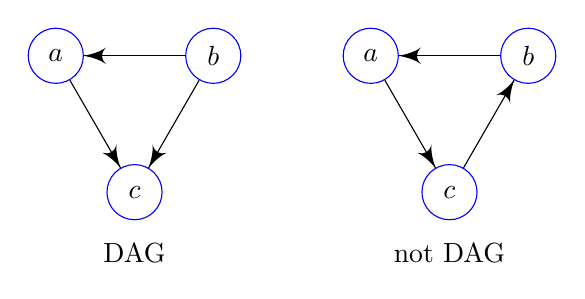
\begin{tikzpicture}
    \node [mstate] (2) at (0, 0) {$a$};
    \node [mstate] (3) at (2, 0) {$b$};

    \node [mstate] (1) at (1, -1.732) {$c$};

    \draw [->] (2) -- (1);
    \draw [->] (3) -- (1);
    \draw [->] (3) -- (2);

    \node at (1, -2.5) {DAG};
    \begin{scope}[shift={(4, 0)}]
      \node [mstate] (2) at (0, 0) {$a$};
      \node [mstate] (3) at (2, 0) {$b$};

      \node [mstate] (1) at (1, -1.732) {$c$};

      \draw [->] (2) -- (1);
      \draw [->] (1) -- (3);
      \draw [->] (3) -- (2);

      \node at (1, -2.5) {not DAG};
    \end{scope}
  \end{tikzpicture}
\end{center}

We will use directed acyclic graphs to encode causal structures, where we have a path from $a$ to $b$ if $a$ ``affects'' $b$.

\begin{defi}[Structural equation model (SEM)]\index{structural equation model}\index{SEM}
  A \emph{structural equation model} $\mathcal{S}$ for a random vector $Z \in \R^p$ is a collection of equations
  \[
    Z_k = h_k(Z_{p_k}, \varepsilon_k),
  \]
  where $k = 1, \ldots, p$ and $\varepsilon_1, \ldots, \varepsilon_p$ are independent, and $p_k \subseteq \{1, \ldots, p\} \setminus \{k\}$ and such that the graph with $pa(k) = p_k$ is a directed acyclic graph.
\end{defi}

\begin{eg}
  Consider three random variables:
  \begin{itemize}
    \item $Z_1 = 1$ if a student is taking a course, $0$ otherwise
    \item $Z_2 = 1$ if a student is attending catch up lectures, $0$ otherwise
    \item $Z_3 = 1$ if a student heard about machine learning before attending the course, $0$ otherwise.
  \end{itemize}
  Suppose
  \begin{align*}
    Z_3 &= \varepsilon_3 \sim \Bernoulli(0.25)\\
    Z_2 &= \mathbf{1}_{\{\varepsilon_2(1 + Z_3) > \frac{1}{2}\}},\quad \varepsilon_2 \sim U[0, 1]\\
    Z_1 &= \mathbf{1}_{\{\varepsilon_1(Z_2 + Z_3) > \frac{1}{2}\}},\quad \varepsilon_1 \sim U[0, 1].
  \end{align*}
  This is then an example of a structural equation modelling, and the corresponding DAG is
  \begin{center}
    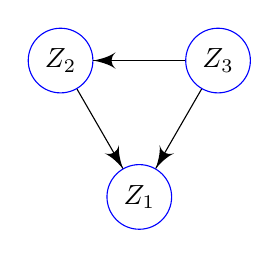
\begin{tikzpicture}
  \node [mstate] (2) at (0, 0) {$Z_2$};
      \node [mstate] (3) at (2, 0) {$Z_3$};

      \node [mstate] (1) at (1, -1.732) {$Z_1$};

      \draw [->] (2) -- (1);
      \draw [->] (3) -- (1);
      \draw [->] (3) -- (2);
    \end{tikzpicture}
  \end{center}
\end{eg}
Note that the structural equation model for $Z$ determines its distribution, but the converse is not true. For example, the following two distinct structural equation give rise to the same distribution:
\begin{align*}
  Z_1 &= \varepsilon & Z_1 &= Z_2\\
  Z_2 &= Z_1 & Z_2 &= \varepsilon
\end{align*}
Indeed, if we have two variables that are just always the same, it is hard to tell which is the cause and which is the effect.

It would be convenient if we could order our variables in a way that $Z_k$ depends only on $Z_j$ for $j < k$. This is known as a \emph{topological ordering}:

\begin{defi}[Descendant]\index{descendant}\index{$\mathrm{de}$}
  We say $k$ is a \emph{descendant} of $j$ if there is a directed path from $j$ to $k$. The set of descendant of $j$ will be denoted $\de(j)$.
\end{defi}

\begin{defi}[Topological ordering]\index{topological ordering}
  Given a DAG $\mathcal{G}$ with $V = \{1, \ldots, p\}$ we say that a permutation $\pi: V \to V$ is a \emph{topological ordering} if $\pi(j) < \pi(k)$ whenever $k \in \de(j)$.
\end{defi}

Thus, given a topological ordering $\pi$, we can write $Z_k$ as a function of $\varepsilon_{\pi^{-1}(1)}, \ldots, \varepsilon_{\pi^{-1}(\pi(k))}$.

How do we understand structural equational models? They give us information that are not encoded in the distribution itself. One way to think about them is via \emph{interventions}. We can modify a structural equation model by replacing the equation for $Z_k$ by setting, e.g.\ $Z_k = a$. In real life, this may correspond to forcing all students to go to catch up workshops. This is called a \term{perfect intervention}\index{intervention!perfect}. The modified SEM gives a new joint distribution for $Z$. Expectations or probabilities with respect to the new distribution are written by adding ``$\ddo(Z_k = a)$''. For example, we write
\[
  \E(Z_j \mid \ddo(Z_k = a)).
\]
In general, this is different to $\E(Z_j \mid Z_k = a)$, since, for example, if we conditioned on $Z_2 = a$ in our example, then that would tell us something about $Z_3$.

\begin{eg}
  After the intervention $\ddo(Z_2 = 1)$, i.e.\ we force everyone to go to the catch-up lectures, we have a new SEM with
  \begin{align*}
    Z_3 &= \varepsilon_3 \sim \Bernoulli(0.25)\\
    Z_2 &= 1\\
    Z_1 &= \mathbf{1}_{\varepsilon_1 (1 + Z_3) > \frac{1}{2}}, \quad \varepsilon_1 \sim U[0, 1].
  \end{align*}
  Then, for example, we can compute
  \[
    \P(Z_1 = 1 \mid \ddo(Z_2 = 1)) = \frac{1}{2} \cdot \frac{3}{4} + \frac{3}{4} + \frac{1}{4} = \frac{9}{16},
  \]
  and by high school probability, we also have
  \[
    \P(Z_1 = 1 \mid Z_2 = 1) = \frac{7}{12}.
  \]
\end{eg}

To understand the DAGs associated to structural equation models, we would like to come up with Markov properties analogous to what we had for undirected graphs. This, in particular, requires the correct notion of ``separation'', which we call d-separation. Our notion should be such that if $S$ d-separates $A$ and $B$ in the DAG, then $Z_A$ and $Z_B$ are conditionally independent given $Z_S$. Let's think about some examples. For example, we might have a DAG that looks like this:
\begin{center}
  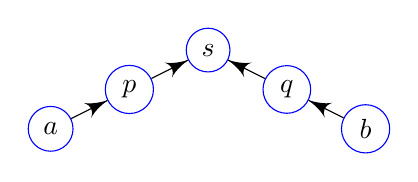
\begin{tikzpicture}
    \node [msstate] (1) at (-2, 0) {$a$};
    \node [msstate] (2) at (-1, 0.5) {$p$};
    \node [msstate] (3) at (0, 1) {$s$};
    \node [msstate] (4) at (1, 0.5) {$q$};
    \node [msstate] (5) at (2, 0) {$b$};

    \draw [->] (1) -- (2);
    \draw [->] (2) -- (3);
    \draw [->] (4) -- (3);
    \draw [->] (5) -- (4);
  \end{tikzpicture}
\end{center}
Then we expect that
\begin{enumerate}
  \item $Z_a$ and $Z_s$ are not independent;
  \item $Z_a$ and $Z_s$ are independent given $Z_q$;
  \item $Z_a$ and $Z_b$ are independent;
  \item $Z_a$ and $Z_b$ are not independent given $Z_s$.
\end{enumerate}
We can explain a bit more about the last one. For example, the structural equation model might telling us $Z_s = Z_a + Z_b + \varepsilon$. In this case, if we know that $Z_a$ is large but $Z_s$ is small, then chances are, $Z_b$ is also large (in the opposite sign). The point is that both $Z_a$ and $Z_b$ both contribute to $Z_s$, and if we know one of the contributions and the result, we can say something about the other contribution as well.

Similarly, if we have a DAG that looks like
\begin{center}
  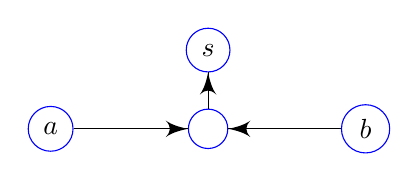
\begin{tikzpicture}
    \node [msstate] (1) at (-2, 0) {$a$};
    \node [msstate] (4) at (0, 0) {};
    \node [msstate] (3) at (0, 1) {$s$};
    \node [msstate] (5) at (2, 0) {$b$};

    \draw [->] (1) -- (4);
    \draw [->] (4) -- (3);
    \draw [->] (5) -- (4);
  \end{tikzpicture}
\end{center}
then as above, we know that $Z_a$ and $Z_b$ are not independent given $Z_s$.

Another example is
\begin{center}
  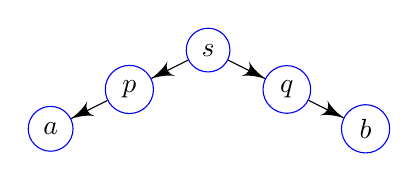
\begin{tikzpicture}
    \node [msstate] (1) at (-2, 0) {$a$};
    \node [msstate] (2) at (-1, 0.5) {$p$};
    \node [msstate] (3) at (0, 1) {$s$};
    \node [msstate] (4) at (1, 0.5) {$q$};
    \node [msstate] (5) at (2, 0) {$b$};

    \draw [->] (2) -- (1);
    \draw [->] (3) -- (2);
    \draw [->] (3) -- (4);
    \draw [->] (4) -- (5);
  \end{tikzpicture}
\end{center}
Here we expect
\begin{itemize}
  \item $Z_a$ and $Z_b$ are not independent.
  \item $Z_a$ and $Z_b$ are independent given $Z_s$.
\end{itemize}
To see (i), we observe that if we know about $Z_a$, then this allows us to predict some information about $Z_s$, which would in turn let us say something about $Z_b$.
\begin{defi}[Blocked]\index{blocked}
  In a DAG, we say a path $(j_1, \ldots, j_m)$ between $j_1$ and $j_m$ is \emph{blocked} by a set of nodes $S$ (with neither $j_1$ nor $j_m$ in $S$) if there is some $j_\ell \in S$ and the path is \emph{not} of the form
  \begin{center}
    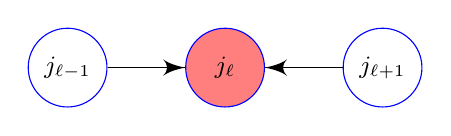
\begin{tikzpicture}
      \node [circle, draw, blue, text=black, minimum width=1cm] (1) at (-2, 0) {\small $j_{\ell - 1}$};
      \node [circle, draw, blue, text=black, minimum width=1cm, fill=red, fill opacity=0.5, text opacity=1] (2) at (0, 0) {\small $j_{\ell}$};
      \node [circle, draw, blue, text=black, minimum width=1cm] (3) at (2, 0) {\small $j_{\ell + 1}$};
      \draw [->] (1) -- (2);
      \draw [->] (3) -- (2);
    \end{tikzpicture}
  \end{center}
  or there is some $j_\ell$ such that the path \emph{is} of this form, but neither $j_\ell$ nor any of its descendants are in $S$.
\end{defi}

\begin{defi}[d-separate]\index{d-separate}
  If $\mathcal{G}$ is a DAG, given a triple of (disjoint) subsets of nodes $A, B, S$, we say $S$ \emph{d-separates} $A$ from $B$ if $S$ blocks every path from $A$ to $B$.
\end{defi}

For convenience, we define
\begin{defi}[$v$-structure]\index{$v$-structure}
  A set of three nodes is called a \emph{$v$-structure} if one node is a child of the two other nodes, and these two nodes are not adjacent.
\end{defi}

It is now natural to define
\begin{defi}[Markov properties]
  Let $P$ be the distribution of $Z$ and let $f$ be the density. Given a DAG $\mathcal{G}$, we say $P$ satisfies
  \begin{enumerate}
    \item the \term{Markov factorization criterion} if
      \[
        f(z_1, \ldots, z_p) = \prod_{k = 1}^p f(z_k \mid z_{\pa(k)}).
      \]
    \item the \term{global Markov property} if for all disjoint $A, B, S$ such that $A, B$ is d-separated by $S$, then $Z_A \amalg Z_B \mid Z_S$.
  \end{enumerate}
\end{defi}

\begin{prop}
  If $P$ has a density with respect to a product measure, then (i) and (ii) are equivalent.
\end{prop}

How does this fit into the structural equation model?

\begin{prop}
  Let $P$ be the structural equation model with DAG $\mathcal{G}$. Then $P$ obeys the Markov factorization property.
\end{prop}

\begin{proof}
  We assume $\mathcal{G}$ is topologically ordered (i.e.\ the identity map is a topological ordering). Then we can always write
  \[
    f(z_1, \ldots, z_p) = f(z_1) f(z_2 \mid z_1) \cdots z(z_p \mid z_1, z_2, \ldots, z_{p - 1}).
  \]
  By definition of a topological order, we know $\pa(k) \subseteq \{1, \ldots, k - 1\}$. Since $Z_k$ is a function of $Z_{\pa(k)}$ and independent noise $\varepsilon_k$. So we know
  \[
    Z_{k} \amalg Z_{\{1, \ldots, p\} \setminus \{k \cup \pa(k)\}} \mid Z_{\pa(k)}.
  \]
  Thus,
  \[
    f(z_{k} \mid z_1, \ldots, z_{k - 1}) = f(z_k \mid z_{\pa(k)}).\qedhere
  \]
\end{proof}

\subsection{The PC algorithm}
We now want to try to find out the structural equation model given some data, and in particular, determine the causal structure. As we previously saw, there is no hope of determining this completely, even if we know the distribution of the $Z$ completely. Let's consider the different obstacles to this problem.

\subsubsection*{Causal minimality}
If $P$ is generated by an SEM with DAG $\mathcal{G}$, then from the above, we know that $P$ is Markov with respect to $\mathcal{G}$. The converse is also true: if $P$ is Markov with respect to a DAG $\mathcal{G}$, then there exists a SEM with DAG $\mathcal{G}$ that generates $P$. This immediately implies that $P$ will be Markov with respect to many DAGs. For example, a DAG whose skeleton is complete will always work. This suggests the following definition:

\begin{defi}[Causal minimality]\index{causal minimality}
  A distribution $P$ satisfies \emph{causal minimality} with respect to $\mathcal{G}$ but not any proper subgraph of $\mathcal{G}$.
\end{defi}

\subsubsection*{Markov equivalent DAGs}

It is natural to aim for finding a causally minimal DAG. However, this does not give a unique solution, as we saw previously with the two variables that are always the same.

In general, two different DAGs may satisfy the same set of d-separations, and then a distribution is Markov with respect to one iff its Markov with respect to the other, and we cannot distinguish between the two.

\begin{defi}[Markov equivalence]\index{Markov equivalence}
  For a DAG $\mathcal{G}$, we let
  \[
    \mathcal{M}(\mathcal{G}) = \{\text{distributions $P$ such that $P$ is Markov with respect to $\mathcal{G}$}\}.
  \]
  We say two DAGs $\mathcal{G}_1, \mathcal{G}_2$ are \emph{Markov equivalent} if $\mathcal{M}(\mathcal{G}_1) = \mathcal{M}(\mathcal{G}_2)$.
\end{defi}
What is nice is that there is a rather easy way of determining when two DAGs are Markov equivalent.

\begin{prop}
  Two DAGs are Markov equivalent iff they have the same skeleton and same set of $v$-structure.
\end{prop}
The set of all DAGs that are Markov equivalent to a given DAG can be represented by a \term{CPDAG} (completed partial DAG), which contains an edge $(j, k)$ iff some member of the equivalence class does.

\subsubsection*{Faithfulness}
To describe the final issue, consider the SEM
\[
  Z_1 = \varepsilon_1,\quad Z_2 = \alpha Z_1 + \varepsilon_2,\quad Z_3 = \beta Z_1 + \gamma Z_2 + \varepsilon_3.
\]
We take $\varepsilon \sim N_3(0, I)$. Then we have $Z = (Z_1, Z_2, Z_3) \sim N(0, \Sigma)$, where
\[
  \Sigma =
  \begin{pmatrix}
    1 & \alpha & \beta + \alpha \gamma\\
    \alpha & \alpha^2 + 1 & \alpha(\beta + \alpha \gamma) + \gamma\\
    \beta + \alpha\gamma & \alpha(\beta + \alpha \gamma) + \gamma & \beta^2 + \gamma^2(\alpha^2 + 1) + 1 + 2\alpha \beta \gamma
  \end{pmatrix}.
\]
\begin{center}
  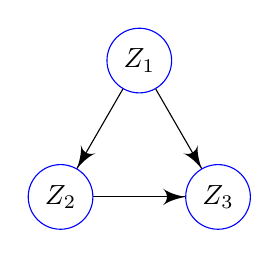
\begin{tikzpicture}
    \node [mstate] (2) at (0, 0) {$Z_2$};
    \node [mstate] (3) at (2, 0) {$Z_3$};

    \node [mstate] (1) at (1, 1.732) {$Z_1$};

    \draw [->] (1) -- (2);
    \draw [->] (1) -- (3);
    \draw [->] (2) -- (3);
  \end{tikzpicture}
\end{center}
Now if we picked values of $\alpha, \beta, \gamma$ such that
\[
  \beta + \alpha \gamma = 0,
\]
then we obtained an extra independence relation $Z_1 \amalg Z_3$ in our system. For example, if we pick $\beta = -1$ and $\alpha, \gamma = 1$, then
\[
  \Sigma =
  \begin{pmatrix}
    1 & 1 & 0\\
    1 & 2 & 1\\
    0 & 1 & 2
  \end{pmatrix}.
\]
While there is an extra independence relation, we cannot remove any edge while still satisfying the Markov property. Indeed:
\begin{itemize}
  \item If we remove $1 \to 2$, then this would require $Z_1 \amalg Z_2$, but this is not true.
  \item If we remove $2 \to 3$, then this would require $Z_2 \amalg Z_3 \mid Z_1$, but we have
    \[
      \var((Z_2, Z_3) \mid Z_1) =
      \begin{pmatrix}
        2 & 1\\
        1 & 2
      \end{pmatrix} -
      \begin{pmatrix}
        1 \\0
      \end{pmatrix}
      \begin{pmatrix}
        1 & 0
      \end{pmatrix} =
      \begin{pmatrix}
        1 & 1\\
        1 & 2
      \end{pmatrix},
    \]
    and this is not diagonal.
  \item If we remove $1 \to 3$, then this would require $Z_1 \amalg Z_3 \mid Z_2$, but
    \[
     \var((Z_1, Z_3) \mid Z_2) =
     \begin{pmatrix}
       1 & 0 \\
       0 & 2
     \end{pmatrix} -
     \frac{1}{2}
     \begin{pmatrix}
       1 \\ 1
     \end{pmatrix}
     \begin{pmatrix}
       1 & 1
     \end{pmatrix},
   \]
   which is again non-diagonal.
\end{itemize}
So this DAG satisfies causal minimality. However, $P$ can also be generated by the structural equation model
\[
  \tilde{Z}_1 = \tilde{\varepsilon}_1,\quad \tilde{Z}_2 = \tilde{Z}_1 + \frac{1}{2} \tilde{Z}_3 + \tilde{\varepsilon}_2,\quad \tilde{Z}_3 = \tilde{\varepsilon}_3,
\]
where the $\tilde{\varepsilon}_i$ are independent with
\[
  \tilde{\varepsilon}_1 \sim N(0, 1),\quad \tilde{\varepsilon}_2 \sim N(0, 2),\quad \tilde{\varepsilon}_3 \sim N(0, \tfrac{1}{2}).
\]
Then this has the DAG
\begin{center}
  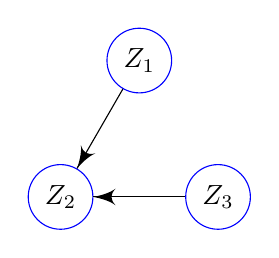
\begin{tikzpicture}
    \node [mstate] (2) at (0, 0) {$Z_2$};
    \node [mstate] (3) at (2, 0) {$Z_3$};

    \node [mstate] (1) at (1, 1.732) {$Z_1$};

    \draw [->] (1) -- (2);
    \draw [->] (3) -- (2);
  \end{tikzpicture}
\end{center}
This is a strictly smaller DAG in terms of the number of edges involved. It is easy to see that this satisfies causal minimality.

\begin{defi}[Faithfulness]\index{faithfulness}
  We say $P$ is \emph{faithful} to a DAG $\mathcal{G}$ if it is Markov with respect to $\mathcal{G}$ and for all $A, B, S$ disjoint, $Z_A \amalg Z_B \mid Z_S$ implies $A, B$ are d-separated by $S$.
\end{defi}

\subsubsection*{Determining the DAG}
We shall assume our distribution is faithful to some $\mathcal{G}_0$, and see if we can figure out $\mathcal{G}_0$ from $P$, or even better, from data.

To find $\mathcal{G}$, the following proposition helps us compute the skeleton:
\begin{prop}
  If nodes $j$ and $k$ are adjacent in a DAG $\mathcal{G}$, then no set can $d$-separate them.

  If they are not adjacent, and $\pi$ is a topological order for $\mathcal{G}$ with $\pi(j) < \pi(k)$, then they are $d$-separated by $\pa(k)$.
\end{prop}

\begin{proof}
  Only the last part requires proof. Consider a path $j = j_1, \ldots, j_m = k$. Start reading the path from $k$ and go backwards. If it starts as $j_{m - 1} \to k$, then $j_{m - 1}$ is a parent of $k$ and blocks the path. Otherwise, it looks like $k \to j_{m - 1}$.

  We keep going down along the path until we first see something of the form
  \begin{center}
    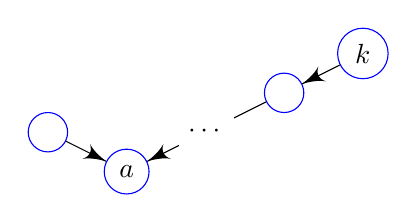
\begin{tikzpicture}
      \node [msstate] (end) at (2, 1) {$k$};
      \node [msstate] (1) at (1, 0.5) {};
      \node [msstate] (2) at (-1, -0.5) {$a$};

      \node [msstate] (start) at (-2, 0) {};

      \draw [->] (end) -- (1);
      \draw [->] (1) -- (2) node [pos=0.5, fill=white] {$\cdots$};
      \draw [->] (start) -- (2);
    \end{tikzpicture}
  \end{center}
  Thus must exist, since $j$ is not a descendant of $k$ by topological ordering. So it suffices to show that $a$ does not have a descendant in $\pa(k)$, but if it did, then this would form a closed loop.
\end{proof}

Finding the $v$-structures is harder, and at best we can do so up to Markov equivalence. To do that, observe the following:
\begin{prop}
  Suppose we have $j - \ell - k$ in the skeleton of a DAG.
  \begin{enumerate}
    \item If $j \to \ell \leftarrow k$, then no $S$ that d-separates $j$ can have $\ell \in S$.
    \item If there exists $S$ that d-separates $j$ and $k$ and $\ell \not \in S$, then $j \to \ell \leftarrow k$.\fakeqed
  \end{enumerate}
\end{prop}
Denote the set of nodes adjacent to the vertex $k$ in the graph $\mathcal{G}$ by $\adj(\mathcal{G}, k)$.

We can now describe the first part of the \term{PC algorithm}, which finds the skeleton of the ``true DAG'':
\begin{enumerate}
  \item Set $\hat{\mathcal{G}}$ to be the complete undirected graph. Set $\ell = -1$.
  \item Repeat the following steps:
    \begin{enumerate}
      \item Set $\ell = \ell + 1$:
      \item Repeat the following steps:
        \begin{enumerate}
          \item Select a new ordered pair of nodes $j, k$ that are adjacent in $\hat{\mathcal{G}}$ and such that $|\adj(\hat{\mathcal{G}}, j) \setminus \{k\}| \geq \ell$.
          \item Repeat the following steps:
            \begin{enumerate}
              \item Choose a new $S \subseteq \adj(\hat{\mathcal{G}}, j) \setminus \{k\}$ with $|S| = \ell$.
              \item If $Z_j \amalg Z_k \mid Z_S$, then delete the edge $jk$, and store $S(k, j) = S(j, k) = S$
              \item Repeat until $j-k$ is deleted or all $S$ chosen.
            \end{enumerate}
          \item Repeat until all pairs of adjacent nodes are inspected.
        \end{enumerate}
      \item Repeat until $\ell \geq p - 2$.
    \end{enumerate}
\end{enumerate}
Suppose $P$ is faithful to a DAG $\mathcal{G}^0$. At each stage of the algorithm, the skeleton of $\mathcal{G}^0$ will be a subgraph of $\hat{\mathcal{G}}$. On the other hand, edges $(j, k)$ remaining at termination will have
\[
  Z_j \amalg Z_k \mid Z_S\text{ for all }S \subseteq (\hat{\mathcal{G}}, k),\quad S \subseteq (\hat{\mathcal{G}}, j).
\]
So they must be adjacent in $\mathcal{G}^0$. Thus, $\hat{\mathcal{G}}$ and $\mathcal{G}_0$ have the same skeleton.

To find the $v$-structures, we perform:
\begin{enumerate}
  \item For all $j-l-k$ in $\hat{\mathcal{G}}$, do:
    \begin{enumerate}
      \item If $\ell \not \in S(j, k)$, then orient $j \to \ell \leftarrow k$.
    \end{enumerate}
\end{enumerate}
This gives us the Markov equivalence class, and we may orient the other edges using other properties like acyclicity.

If we want to apply this to data sets, then we need to apply some conditional independence tests instead of querying our oracle to figure out if things are conditional dependence. However, errors in the algorithm propagate, and the whole process may be derailed by early errors. Moreover, the result of the algorithm may depend on how we iterate through the nodes. People have tried many ways to fix these problems, but in general, this method is rather unstable. Yet, if we have large data sets, this can produce quite decent results.

\section{High-dimensional inference}
\subsection{Multiple testing}
Finally, we talk about high-dimensional inference. Suppose we have come up with a large number of potential drugs, and want to see if they are effective in killing bacteria. Naively, we might try to run a hypothesis test on each of them, using a $p < 0.05$ threshold. But this is a terrible idea, since each test has a $0.05$ chance of giving a false positive, so even if all the drugs are actually useless, we would have incorrectly believed that a lot of them are useful, which is not the case.

In general, suppose we have some null hypothesis $H_1, \ldots, H_m$. By definition, a $p$ value $p_i$ for $H_i$ is a random variable such that
\[
  \P_{H_i}(p_i \leq \alpha) \leq \alpha
\]
for all $\alpha \in [0, 1]$.

Let $m_0 = |I_0|$ be the number of true null hypothesis. Given a procedure for rejecting hypothesis (a \term{multiple testing procedure}), we let $N$ be the number of false rejections (false positives), and $R$ the total number of rejections. One can also think about the number of false negatives, but we shall not do that here.

Traditionally, multiple-testing procedures sought to control the \term{family-wise error rate} (\term{FWER}), defined by $\P(N \geq 1)$. The simplest way to minimize this is to use the \term{Bonferroni correction}, which rejects $H_i$ if $p_i \leq \frac{\alpha}{m}$. Usually, we might have $\alpha \sim 0.05$, and so this would be very small if we have lots of hypothesis (e.g.\ a million). Unsurprisingly, we have
\begin{thm}
  When using the Bonferroni correction, we have
  \[
    \mathrm{FWER} \leq \E(N) \leq \frac{m_0 \alpha}{m} \leq \alpha.
  \]
\end{thm}

\begin{proof}
  The first inequality is Markov's inequality, and the last is obvious. The second follows from
  \[
    \E(N) = \E \left(\sum_{i \in I_0} \mathbf{1}_{p_i \leq \alpha/m}\right) = \sum_{i \in I_0} \P\left(p_i \leq \frac{\alpha}{m}\right) \leq \frac{m_0 \alpha}{m}.\qedhere
  \]
\end{proof}
The Bonferroni is a rather conservative procedure, since all these inequalities can be quite loose. When we have a large number of hypotheses, the criterion for rejection is very very strict. Can we do better?

A more sophisticated approach is the \term{closed testing procedure}. For each non-empty subset $I \subseteq \{1, \ldots, m\}$, we let $H_I$ be the null hypothesis that $H_i$ is true for all $i \in I$. This is known as an \term{intersection hypothesis}. Suppose for each $I \subseteq \{1, \ldots, m\}$ non-empty, we have an $\alpha$-level test $\phi_I$ for $H_I$ (a \term{local test}), so that
\[
  \P_{H_I}(\phi_I = 1) \leq \alpha.
\]
Here $\Phi_I$ takes values in $\{0, 1\}$, and $\phi_I = 1$ means rejection. The closed testing procedure then rejects $H_I$ iff for all $J \supseteq I$, we have $\phi_J = 1$.

\begin{eg}
  Consider the tests, where the red ones are the rejected one:
  \begin{center}
    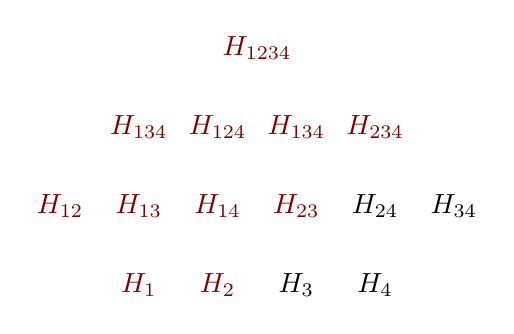
\begin{tikzpicture}
      \node [mred] at (0, 4) {$H_{1234}$};

      \node [mred] at (-1.5, 3) {$H_{134}$};
      \node [mred] at (-0.5, 3) {$H_{124}$};
      \node [mred] at (0.5, 3) {$H_{134}$};
      \node [mred] at (1.5, 3) {$H_{234}$};

      \node [mred] at (-2.5, 2) {$H_{12}$};
      \node [mred] at (-1.5, 2) {$H_{13}$};
      \node [mred] at (-0.5, 2) {$H_{14}$};
      \node [mred] at (0.5, 2) {$H_{23}$};
      \node at (1.5, 2) {$H_{24}$};
      \node at (2.5, 2) {$H_{34}$};

      \node [mred] at (-1.5, 1) {$H_{1}$};
      \node [mred] at (-0.5, 1) {$H_{2}$};
      \node at (0.5, 1) {$H_{3}$};
      \node at (1.5, 1) {$H_{4}$};
    \end{tikzpicture}
  \end{center}
  In this case, we reject $H_1$ but not $H_2$ by closed testing. While $H_{23}$ is rejected, we cannot tell if it is $H_2$ or $H_3$ that should be rejected.
\end{eg}

This might seem like a very difficult procedure to analyze, but it turns out it is extremely simple.
\begin{thm}
  Closed testing makes no false rejections with probability $\geq 1 - \alpha$. In particular, FWER $\leq \alpha$.
\end{thm}

\begin{proof}
  In order for there to be a false rejection, we must have falsely rejected $H_{I_0}$ with the local test, which has probability at most $\alpha$.
\end{proof}

But of course this doesn't immediately give us an algorithm we can apply to data. Different choices for the local test give rise to different multiple testing procedures. One famous example is \term{Holm's procedure}. This takes $\phi_I$ to be the Bonferroni test, where $\phi_I = 1$ iff $p_i \leq \frac{\alpha}{|I|}$ for some $i \in I$.

When $m$ is large, then we don't want to compute all $\phi_I$, since there are $2^I$ computations to do. So we might want to find a shortcut. With a moment of thought, we see that Holm's procedure amounts to the following:
\begin{itemize}
  \item Let $(i)$ be the index of the $i$th smallest $p$-value, so $p_{(1)} \leq p_{(2)} \leq \cdots \leq p_{(m)}$.
  \item Step $1$: If $p_{(1)} \leq \frac{\alpha}{m}$, then reject $H_{(1)}$ and go to step $2$. Otherwise, accept all null hypothesis.
  \item Step $i$: If $p_{(i)} \leq \frac{\alpha}{m - i + 1}$, then reject $H_{(i)}$ and go to step $i + 1$. Otherwise, accept $H_{(i)}, H_{(i + 1)}, \ldots, H_{(m)}$.
  \item Step $m$: If $p_{(m)} \leq \alpha$, then reject $H_{(m)}$. Otherwise, accept $H_{(m)}$.
\end{itemize}
The interesting thing about this is that it has the same bound on FWER as the Bonferroni correction, but the conditions here are less lenient.

But if $m$ is very large, then the criterion for accepting $p_{(1)}$ is still quite strict. The problem is that controlling FWER is a very strong condition. Instead of controlling the probability that there is one false rejection, when $m$ is large, it might be more reasonable to control the proportion of false discoveries. Many modern multiple testing procedures aim to control the \term{false discovery rate}
\[
  \mathrm{FDR} = \E\left(\frac{N}{\max \{R, 1\}}\right).
\]
The funny maximum in the denominator is just to avoid division by zero. When $R = 0$, then we must have $N = 0$ as well, so what is put in the denominator doesn't really matter.

The \term{Benjamini--Hochberg procedure} attempts to control the FDR at level $\alpha$ and works as follows:
\begin{itemize}
  \item Let $\hat{k} = \max \left\{i: p_{(i)} \leq \frac{\alpha i}{m}\right\}$. Then reject $M_{(1)}, \ldots, H_{(\hat{k})}$, or accept all hypothesis if $\hat{k}$ is not defined.
\end{itemize}

Under certain conditions, this does control the false discovery rate.
\begin{thm}
  Suppose that for each $i \in I_0$, $p_i$ is independent of $\{p_j: j \not= i\}$. Then using the Benjamini--Hochberg procedure, the false discovery rate
  \[
    FDR = \E \frac{N}{\max (R, 1)} \leq \frac{\alpha M_0}{M} \leq \alpha.
  \]
\end{thm}
Curiously, while the proof requires $p_i$ to be independent of the others, in simulations, even when there is no hope that the $p_i$ are independent, it appears that the Benjamini--Hochberg still works very well, and people are still trying to understand what it is that makes Benjamini--Hochberg work so well in general.

\begin{proof}
  The false discovery rate is
  \begin{align*}
    \E \frac{N}{\max (R, 1)} &= \sum_{r = 1}^M \E \frac{N}{r} \mathbf{1}_{R = r}\\
    &= \sum_{r = 1}^m \frac{1}{r} \E \sum_{i \in I_0} \mathbf{1}_{p_i \leq \alpha r/M} \mathbf{1}_{R = r}\\
    &= \sum_{i \in I_0} \sum_{r = 1}^M \frac{1}{r} \P\left(p_i \leq \frac{\alpha r}{m}, R = r\right).
  \end{align*}
  The brilliant idea is, for each $i \in I_0$, let $R_i$ be the number of rejections when applying a modified Benjamini--Hochberg procedure to $p^{\setminus i} = \{p_1, \ldots, p_M\} \setminus \{p_i\}$ with cutoff
  \[
    \hat{k}_i = \max \left\{j: p_{(j)}^{\setminus i} \leq \frac{\alpha (j + 1)}{m}\right\}
  \]
  We observe that for $i \in I_0$ and $r \geq 1$, we have
  \begin{align*}
    \left\{ p_i \leq \frac{\alpha r}{m},\, R = r\right\} &= \left\{ p_i \leq \frac{ar}{m},\, p_{(r)} \leq \frac{\alpha r}{m},\, p_{(s)} > \frac{\alpha s}{m}\text{ for all }s \geq r\right\}\\
    &= \left\{p_i \leq \frac{\alpha r}{m},\, p_{(r - 1)}^{\setminus i} \leq \frac{\alpha r}{m},\, p^{\setminus i}_{(s - 1)} > \frac{\alpha s}{m}\text{ for all }s > r\right\}\\
    &= \left\{p_i \leq \frac{\alpha r}{m},\, R_i = r - 1\right\}.
  \end{align*}
  The key point is that $R_i = r - 1$ depends only on the other $p$-values. So the FDR is equal to
  \begin{align*}
    \mathrm{FDR} &= \sum_{i \in I_0} \sum_{r = 1}^M \frac{1}{r} \P\left(p_i \leq \frac{\alpha r}{M}, R_i = r - 1\right)\\
    &= \sum_{i \in I_0} \sum_{r = 1}^M \frac{1}{r} \P \left(p_i \leq \frac{\alpha r}{m}\right) \P(R_i = r - 1)\\
    \intertext{Using that $\P(p_i \leq \frac{\alpha r}{m}) \leq \frac{\alpha r}{m}$ by definition, this is}
    &\leq \frac{\alpha }{M} \sum_{i \in I_0} \sum_{r = 1}^m \P(R_i = r - 1)\\
    &= \frac{\alpha}{M} \sum_{i \in I_0} \P(R_i \in \{0, \ldots, m - 1\})\\
    &= \frac{\alpha M_0}{M}.\qedhere
  \end{align*}
\end{proof}
This is one of the most used procedures in modern statistics, especially in the biological sciences.


\subsection{Inference in high-dimensional regression}
We have more-or-less some answer as to how to do hypothesis testing, given that we know how to obtain these $p$-values. But how do we obtain these in the first place?

For example, we might be trying to do regression, and are trying figure out which coefficients are non-zero. The low dimension setting, with the normal linear model $Y = X\beta^0 + \varepsilon$, where $\varepsilon \sim N_n(0, \sigma^2 I)$. In the low-dimensional setting, we have $\sqrt{n}(\hat{\beta}^{OLS} - \beta^0) \sim N_p(0, \sigma^2(\frac{1}{n} X^T X)^{-1})$. Since this does not depend on $\beta^0$, we can use this to form confidence intervals and hypothesis tests.

However, if we have more coefficients than there are data points, then we can't do ordinary least squares. So we need to look for something else. For example, we might want to replace the OLS estimate with the Lasso estimate. However, $\sqrt{n}(\hat{\beta}_\lambda^L - \beta^0)$ has an intractable distribution. In particular, since $\hat{\beta}_\lambda^L$ has a bias, the distribution will depend on $\beta^0$ in a complicated way.

The recently introduced \term{debiased Lasso} tries to overcomes these issues. See \emph{van de Geer, B\"uhlmann, Ritov, Dezeure} (2014) for more details. Let $\hat{\beta}$ be the Lasso solution at $\lambda > 0$. Recall the KKT conditions that says $\hat{\nu}$ defined by
\[
  \frac{1}{n} X^T (Y - X \hat{\beta}) = \lambda \hat{\nu}
\]
satisfies $\|\hat{\nu}\|_\infty \leq 1$ and $\hat{\nu}_{\hat{S}} = \sgn (\hat{\beta}_{\hat{S}})$, where $\hat{S} = \{k : \hat{\beta}_k \not= 0\}$.

We set $\hat{\Sigma} = \frac{1}{n} X^T X$. Then we can rewrite the KKT conditions as
\[
  \hat{\Sigma} (\hat{\beta} - \beta^0) + \lambda \hat{\nu} = \frac{1}{n} X^T \varepsilon.
\]
What we are trying to understand is $\hat{\beta} - \beta^0$. So it would be nice if we can find some sort of inverse to $\hat{\Sigma}$. If so, then $\hat{\beta} - \beta^0$ plus some correction term involving $\hat{v}$ would then be equal to a Gaussian.

Of course, the problem is that in the high dimensional setting, that $\hat{\Sigma}$ has no hope of being invertible. So we want to find some approximate inverse $\hat{\Theta}$ so that the error we make is not too large. If we are equipped with such a $\hat{\Theta}$, then we have
\[
  \sqrt{n} (\hat{\beta} + \lambda \hat{\Theta} \hat{\nu} - \beta^0) = \frac{1}{\sqrt{n}} \hat{\Theta} X^T \varepsilon + \Delta,
\]
where
\[
  \Delta = \sqrt{n}(\hat{\Theta} \hat{\Sigma} - I)(\beta^0 - \hat{\beta}).
\]
We hope we can choose $\hat{\Theta}$ so that $\delta$ is small. We can then use the quantity
\[
  b = \hat{\beta} + \lambda \hat{\Theta} \hat{\nu} = \hat{\beta} + \frac{1}{n} \hat{\Theta} X^T (Y - X \hat{\beta})
\]
as our modified estimator, called the \term{debiased Lasso}.

How do we bound $\Delta$? We already know that (under compatibility and sparsity conditions), we can make the $\ell_1$ norm of $\|\beta^0 - \hat{\beta}\|$ small with high probability. So if the $\ell_\infty$ norm of each of the rows of $\hat{\Theta} \hat{\Sigma} - 1$ is small, then H\"older allows us to bound $\Delta$.

Write $\hat{\theta}_j$ for the $j$th row of $\hat{\Theta}$. Then
\[
  \|(\hat{\Sigma} \hat{\Theta}^T)_j - I \|_\infty \leq \eta
\]
is equivalent to $|(\hat{\Sigma} \hat{\Theta}^T)_{kj}| \leq \eta$ for $k \not= j$ and $|(\hat{\Sigma} \hat{\Theta}^T)_{jj} - 1 | \leq \eta$. Using the definition of $\hat{\Sigma}$, these are equivalent to
\[
  \frac{1}{n}|X_k^T X \hat{\theta}_j| \leq \eta,\quad \left|\frac{1}{n} X^T_j X \hat{\theta}_j - 1 \right| \leq \eta.
\]
The first is the same as saying
\[
  \frac{1}{n} \|X_{-j}^T X \hat{\theta}_j\|_\infty \leq \eta.
\]
This is quite reminiscent of the KKT conditions for the Lasso. So let us define
\begin{align*}
  \hat{\gamma}^{(j)} &= \argmin_{\gamma \in \R^{p - 1}} \left\{\frac{1}{2n} \|X_j - X_{-j} \gamma\|_2^2 + \lambda_j \|\gamma\|_1\right\}\\
  \hat{\tau}_j^2 &= \frac{1}{n} X_j^T (X_j - X_{-j} \hat{\gamma}^{(j)}) = \frac{1}{n} \|X_j - X_{-j} \hat{\gamma}^{(j)}\|_2^2 + \lambda_j \|\hat{\gamma}^{(j)}\|_1.
\end{align*}
The second equality is an exercise on the example sheet.

We can then set
\[
  \hat{\theta}_j = -\frac{1}{\hat{\tau}_j^2} (\hat{\gamma}_1^{(j)}, \ldots, \hat{\gamma}_{j - 1}^{(j)}, -1, \hat{\gamma}_j^{(j)}, \ldots, \hat{\gamma}_{p - 1}^{(j)})^T.
\]
The factor is there so that the second inequality holds.

Then by construction, we have
\[
  X \hat{\theta}_j = \frac{X_j - X_{-j} \hat{\gamma}^{(j)}}{X^T_j(X - X_{-j} \hat{\gamma}^{(j)})/n}.
\]
Thus, we have $X_j^T X \hat{\theta}_j n = 1$, and by the KKT conditions for the Lasso, we have
\[
  \frac{\hat{\tau}_j}{n} \|X_{-j}^T X \hat{\theta}_j\|_{\infty} \leq \lambda_j.
\]
Thus, with the choice of $\hat{\Theta}$ above, we have
\[
  \|\Delta\|_{\infty} \leq \sqrt{n} \|\hat{\beta} - \beta^0\|_1 \max_j \frac{\lambda_j}{\hat{\tau}_j^2}.
\]
Now this is good as long as we can ensure $\frac{\lambda_j}{\hat{\tau}_j^2}$ to be small. When is this true?

We can consider a random design setting, where each row of $X$ is iid $N_p(0, \Sigma)$ for some positive-definite $\Sigma$. Write $\Omega = \Sigma^{-1}$.

Then by our study of the neighbourhood selection procedure, we know that for each $j$, we can write
\[
  X_j = X_{-j} \gamma^{(j)} + \varepsilon^{(j)},
\]
where $\varepsilon_i^{(j)}\mid X_{-j} \sim N(0, \Omega_{jj}^{-1})$ are iid and $\gamma^{(j)} = - \Omega_{jj}^{-1} \Omega_{-j, j}$. To apply our results, we need to ensure that $\gamma^{(j)}$ are sparse. Let use therefore define
\[
  s_j = \sum_{k \not= j} \mathbf{1}_{\Omega_{jk} \not =0},
\]
and set $s_{max} = \max (\max_j s_j, s)$.

\begin{thm}
  Suppose the maximum eigenvalue of $\Sigma$ is always at least $c_{min} > 0$ and $\max_j \Sigma_{jj} \leq 1$. Suppose further that $s_{max} \sqrt{\log (p)/n} \to 0$. Then there exists constants $A_1, A_2$ such that setting $\lambda = \lambda_j = A_1 \sqrt{\log(p) /n}$, we have
  \begin{align*}
    \sqrt{n} (\hat{b} - \beta^0) &= W + \Delta\\
    W\mid X &\sim N_p(0, \sigma^2 \hat{\Theta} \hat{\Sigma} \hat{\Theta}^T),
  \end{align*}
  and as $n, p \to \infty$,
  \[
    \P\left(\|\Delta\|_\infty > A_2 s \frac{\log(p)}{\sqrt{n}}\right) \to 0.
  \]
\end{thm}
Note that here $X$ is not centered and scaled.

We see that in particular, $\sqrt{n}(\hat{b}_j - \beta_j^0) \sim N(0, \sigma^2(\hat{\Theta} \hat{\Sigma} \hat{\Theta}^T)_{jj})$. In fact, one can show that
\[
  d_j = \frac{1}{n} \frac{\|X_j - X_{-j} \hat{\gamma}^{(j)}\}_2^2}{\hat{\tau}_j^2}.
\]
This suggests an approximate $(1 - \alpha)$-level confidence interval for $\beta^0_j$,
\[
  \mathrm{CI} = \left(b_j - Z_{\alpha/2} \sigma \sqrt{d_j/n}, \hat{b}_j + Z_{\alpha/2} \sigma \sqrt{d_j/n}\right),
\]
where $Z_\alpha$ is the upper $\alpha$ point of $N(0, 1)$. Note that here we are getting confidence intervals of width $\sim \sqrt{1/n}$. In particular, there is no $\log p$ dependence, if we are only trying to estimate $\beta^0_j$ only.

\begin{proof}
  Consider the sequence of events $\Lambda_n$ defined by the following properties:
  \begin{itemize}
    \item $\phi_{\hat{\Sigma}, s} \geq c_{min}/2$ and $\phi^2_{\hat{\Sigma}_{-j, -j}, s_j} \geq c_{min}/2$ for all $j$
    \item $\frac{2}{n} \|X^T \Sigma\|_\infty \leq \lambda$ and $\frac{2}{n} \|X_{-j}^T \varepsilon^{(j)} \|_\infty \leq \lambda$.
    \item $\frac{1}{n} \Sigma^{(j)} \|_2^2 \geq (\Omega_{jj})^{-1} (1 - 4 \sqrt{(\log p) / n})$
  \end{itemize}
%  The idea of the last condition is that we hope $\|X_j - X_{-j} \hat{\gamma}^{(j)}\|_2^2$ would be close to $\varepsilon$, so we want $\hat{\gamma}^{(j)}$ to be not too far off from the what it ought to be, and

  Question 13 on example sheet 4 shows that $\P(\Lambda_n) \to 1$ for $A_1$ sufficiently large. So we will work on the event $\Lambda_n$.

  By our results on the Lasso, we know
  \[
    \|\beta^0 - \hat{\beta}\|_1 \leq c_1 s \sqrt{\log p / n}.
  \]
  for some constant $c_1$. We now seek a lower bound for $\hat{\tau}_j^2$. Consider linear models
  \[
    X_j = X_{-j} \gamma^{(j)} + \varepsilon^{(j)},
  \]
  where the sparsity of $\gamma^{(j)}$ is $s_j$, and $\varepsilon_i^{(j)}| X_{-j} \sim N(0, \Omega_{jj}^{-1})$. Note that
  \[
    \Omega_{jj}^{-1} = \var (X_{ij} \mid X_{i, -j}) \leq \var(X_{ij}) = \Sigma_{ij} \leq A.
  \]
  Also, the maximum eigenvalue of $\Omega$ is at most $c_{min}^{-1}$. So $\Omega_{jj} \leq c_{min}^{-1}$. So $\Omega_{jj}^{-1} \geq c_{min}$. So by Lasso theory, we know
  \[
    \|\gamma^{(j)} - \hat{\gamma}^{(j)}\|_1 \leq c_2 s_j \sqrt{\frac{\log p}{n}}
  \]
  for some constant $c_2$. Then we have
  \begin{align*}
    \hat{\tau}_j^2 &= \frac{1}{n} \|X_j - X_{-j} \hat{\gamma}^{(j)} \|_2^2 + \lambda \|\hat{\gamma}^{(j)} \|_1\\
    &\geq \frac{1}{n} \|\varepsilon^{(j)} + X_{-j} (\gamma^{(j)} - \hat{\gamma}^{(j)})\|_2^2\\
    &\geq \frac{1}{n} \|\varepsilon^{(j)}\|_2^2 - \frac{2}{n} \|X_{-j}^T \varepsilon^{(j)}\|_\infty \|\gamma^{(j)} - \hat{\gamma}^{(j)}\|_1\\
    &\geq \Omega_{jj}^{-1} \left(1 - 4\sqrt{\frac{\log p}{n}}\right) - c_2 s_j \sqrt{\frac{\log p}{n}} + A_1 \sqrt{\frac{\log p}{n}}
  \end{align*}
  In the limit, this tends to $\Omega_{jj}^{-1}$. So for large $n$, this is $\geq \frac{1}{2} \Omega_{jj}^{-1} \geq \frac{1}{2} c_{min}$.

  Thus, we have
  \[
    \|\Delta\|_\infty \leq 2\lambda \sqrt{n} c_1 s \sqrt{\frac{\log p}{n}} c_{min}^{-1} = A_2 s \frac{\log p}{\sqrt{n}}.\qedhere
  \]
\end{proof}


\printindex
\end{document}
